%!TeX root = SAS2017_18_senacheribbe.tex

\graphicspath{{graphics/task1/}}
\chapter{Task 1: analysis of filtered periodic signals}
\section{Description of the task}
The scope of this task is to analyze the response of the IIR filter with transfer function 
\begin{equation}
\label{eq:t1_z_filter}
H(z)=\frac{\alpha z}{z-a}
\end{equation}
where $a$ is a parameter that can assume the values $a= [-0.9, -0.8, -0.4, 0, 0.4, 0.8, 0.9]$ and $\alpha=1-a$ to satisfy the condition $H(z=1)=1$.\\
To test the filter, two periodic signals must be used as input: a square wave (period 64, duty cycle 50\%, mean value 0, avg power 1) and a sinusoidal wave (period 64, mean value 0, average power 1).\\
It is required to evaluate the output of the filter in MATLAB for both input signals (consider 8 periods) and for all values of $a$, using the finite difference equation corresponding to \cref{eq:t1_z_filter}.\\
Then the absolute value of the DFT of the input and output signals should be calculated and plotted, again for all values of $a$ of the filter.\\
The output of the filter with $a=-0.8$ and $a=0.8$ with the one-sided sinusoidal signal has to be compared with the response to a theoretical sinusoid with infinite extension.\\
Finally the average power of all output signals should be plotted with respect to $a$. 

\section{MATLAB code}
\lstinputlisting[style= Matlab-editor,  basicstyle=\small]{../final_project_task1.m}

\pagebreak
\section{Results and comments}
\subsection{Filter definition}
To satisfy the requirements on the input signals, we use the following expressions for the square wave
\begin{gather}
x_{sw}[n]=\sum_{s=0}^{N_p-1} q[n-sN]  \text{ , }\qquad  q[n]=\begin{cases}
1 & \text{if $0\le n < N/2$}\\
-1 & \text{if $N/2\le n < N$}
\end{cases}
\end{gather}
and for the sinusoidal wave
\begin{equation}
x_{sin}[n]= \sqrt{2}  sin \left(\frac{2 \pi}{N} n\right) \quad \text{for } 0\le n < N N_p
\end{equation}
where $N=64$ the period of both signal, and $N_p=8$ is the number of periods considered.\\
The filter in \cref{eq:t1_z_filter} can be written using the corresponding finite difference equation
\begin{equation}\label{eq:t1_fde}
y[n]=\alpha x[n] + a y[n-1] = (1-a) x[n] + a y[n-1]
\end{equation}
\subsection{Evaluation of the outputs}
The expression in \cref{eq:t1_fde} was coded into the script, and by iterating for all possible values of $a$, the filter outputs were computed for both type of inputs. \\
The DFT of one period of the input and output signals were also computed using the MATLAB command \textit{fft()}. For the outputs, the last simulated period was considered, so to reduce the effect of transients.\\
\\
From \cref{fig:t1_io_sw_1} to \cref{fig:t1_io_sw_7} (7 figures) the responses to the square wave input are shown with their DFT, while from \cref{fig:t1_io_sin_1} to \cref{fig:t1_io_sin_7} (7 figures) the one corresponding to the sinusoidal input are shown.\\
\\
For $a$ negative, the square wave signal is highly distorted, producing alternating peaks. In the DFT, this corresponds to the amplification of high frequencies.
For $a=0$, the filter becomes $y[n]=x[n]$, and the output is the same as the input.
For $a$ positive, the low-pass behavior is clearly visible from the plot of y[n]. Indeed the DFT presents the attenuation of high frequencies.\\
\\
For the sinusoidal input with negative values of the parameter $a$, we notice very little changes on the output, while for $a=0$ the same argument done for the square wave holds: the filter tf is 1 and the output is equal to the input. For $a>0$, we notice instead an attenuation in magnitude and a phase shift of the sinusoid.
\subsection{Theoretical sinusoid}
For evaluating analytically the response of the filter to a sinusoidal signal with infinite extension we use
\begin{equation}\label{eq:t1_theo_sin}
y[n]=\sqrt 2 |H(e^{j 2 \pi /N })|  sin(2\pi n/N + \angle H(e^{j 2 \pi /N }))
\end{equation}
since we can recall from theory that the sinusoid can be written as sum of two complex exponential, eigenfunctions of the filter.
Using MATLAB to compute \cref{eq:t1_theo_sin} for $a=-0.8$ and $a=0.8$, the results are plotted in \cref{fig:t1_theor_sin_2,fig:t1_theor_sin_6} (only first 2 periods), together with the filter response to a one-sided sinusoid. The simulated outputs differ from the theoretical ones just for the first half period, when the transients are not extinguished yet.
\begin{figure} [H]
	\centering
	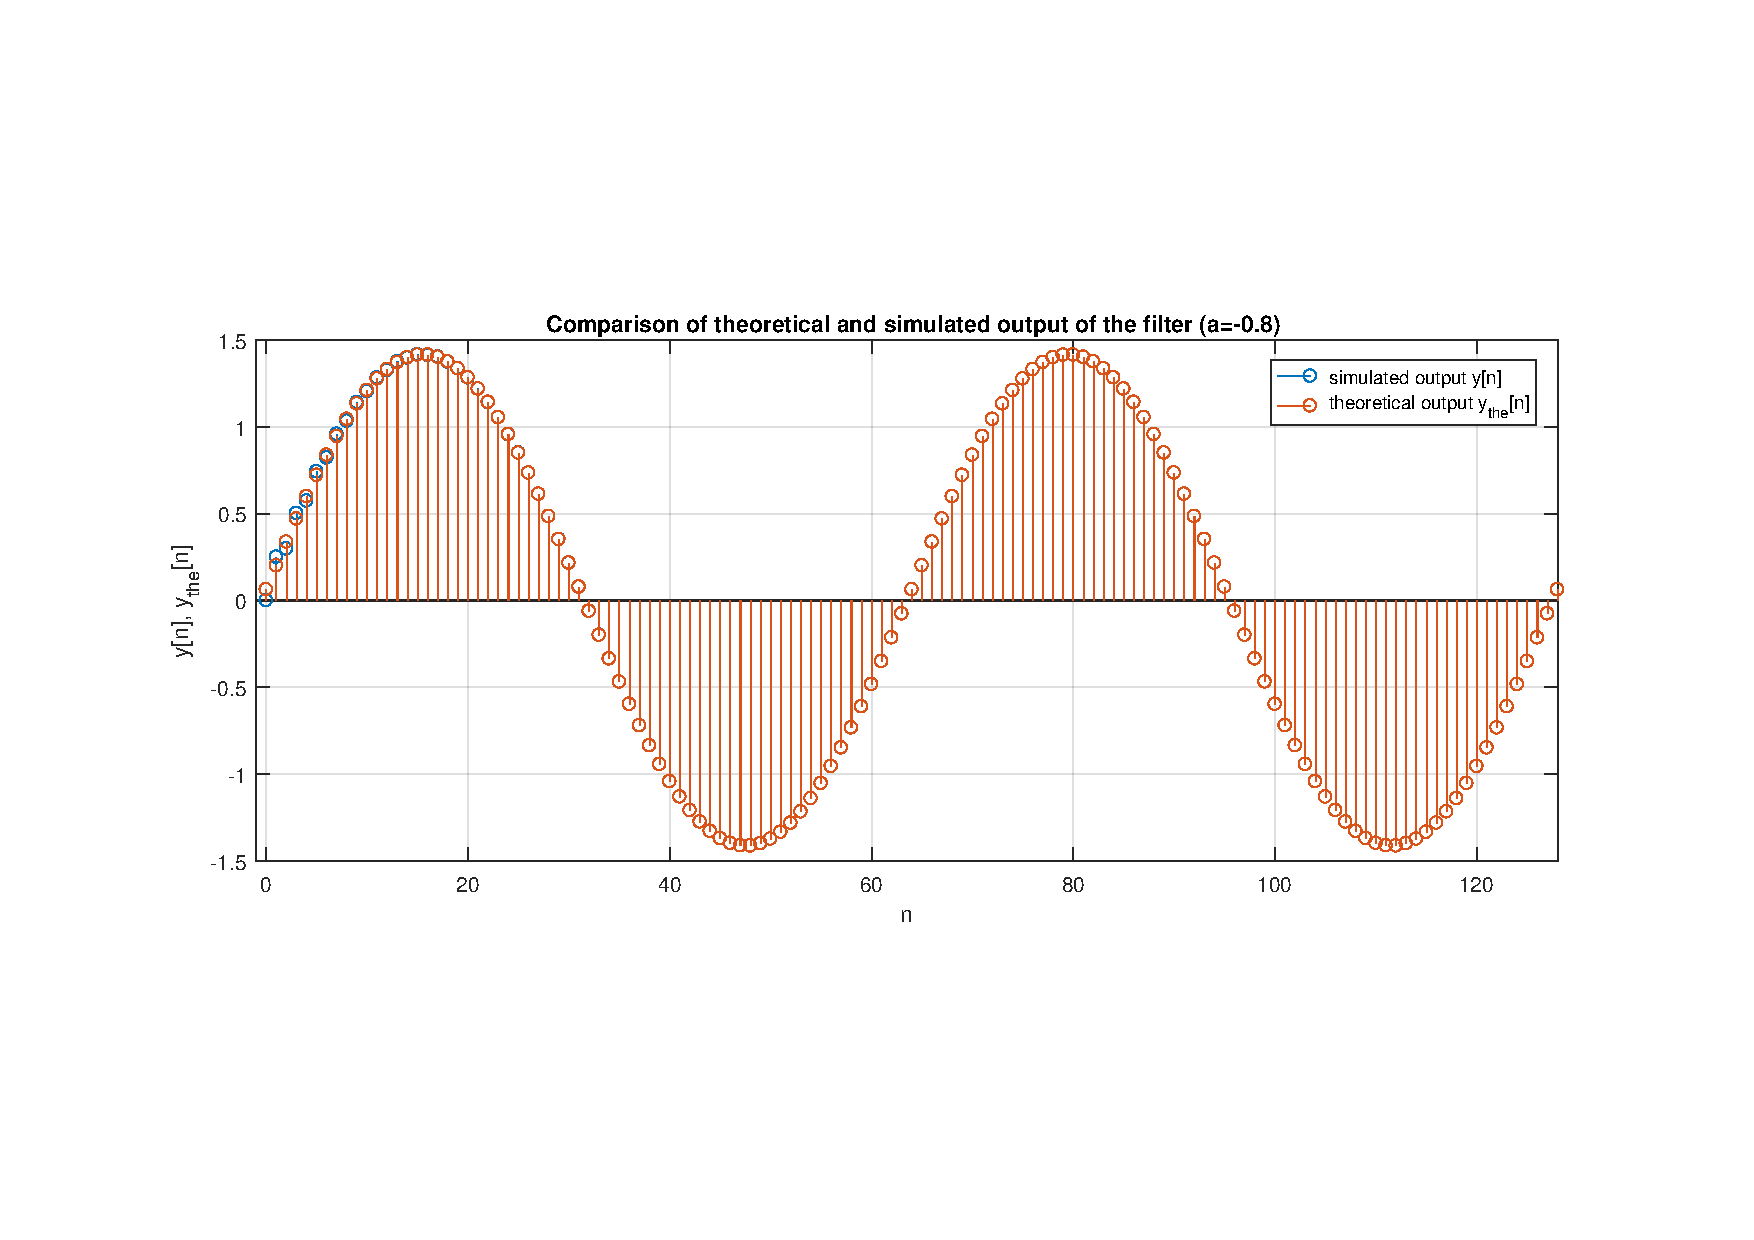
\includegraphics[trim={2.5cm 5cm 2.5cm 5cm}, clip, width=0.65\linewidth]{theor_sin_2}
	\caption{Comparison of theoretical and simulated output, sinusoidal wave input, $a=-0.8$}
	\label{fig:t1_theor_sin_2}
\end{figure}


\begin{figure} [H]
	\centering
	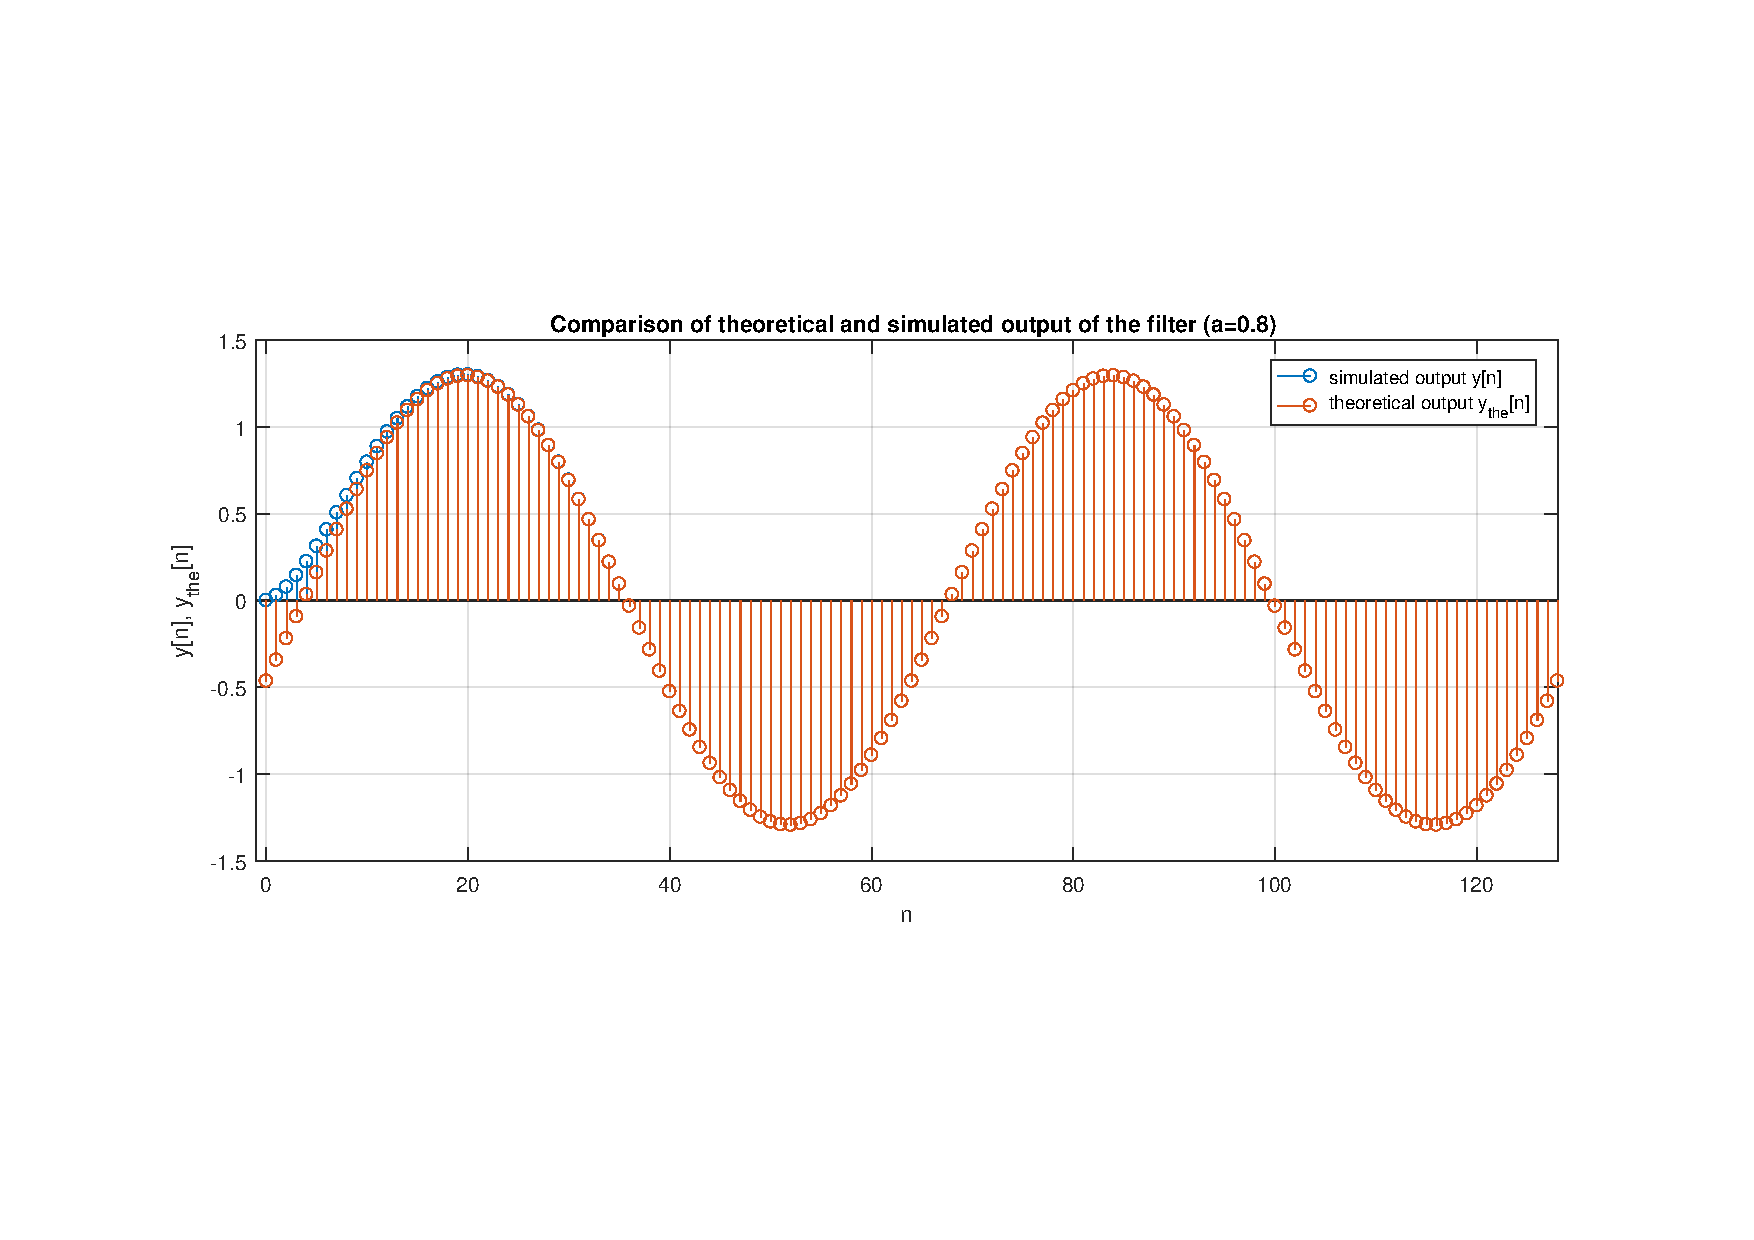
\includegraphics[trim={2.5cm 5cm 2.5cm 5cm}, clip, width=0.65\linewidth]{theor_sin_6}
	\caption{Comparison of theoretical and simulated output, sinusoidal wave input, $a=0.8$}
	\label{fig:t1_theor_sin_6}
\end{figure}
\subsection{Average power}
To measure the average power, only the last simulated period of the outputs was considered, as done previously with the DFT. Since the signals are periodic, it is sufficient to measure the energy of one period and divide by the period itself
\begin{equation}
\mathcal{P}=\frac{\mathcal{E}(y_t)}{N}=\frac{y_t^\dagger y_t}{N}
\end{equation}
where $y_t$ is the signal truncated on the last period considered in the simulation.
The results for the energies are shown in \cref{fig:t1_power}. It can be noticed that for the square wave input with negative $a$, we have higher average power (amplification), due to presence of the previously described peaks. For both types of signal the average power of the output is attenuated for $a$ positive, and it is equal to 1 for $a=0$ (same as the average power of the input).
\begin{figure} [H]
	\centering
	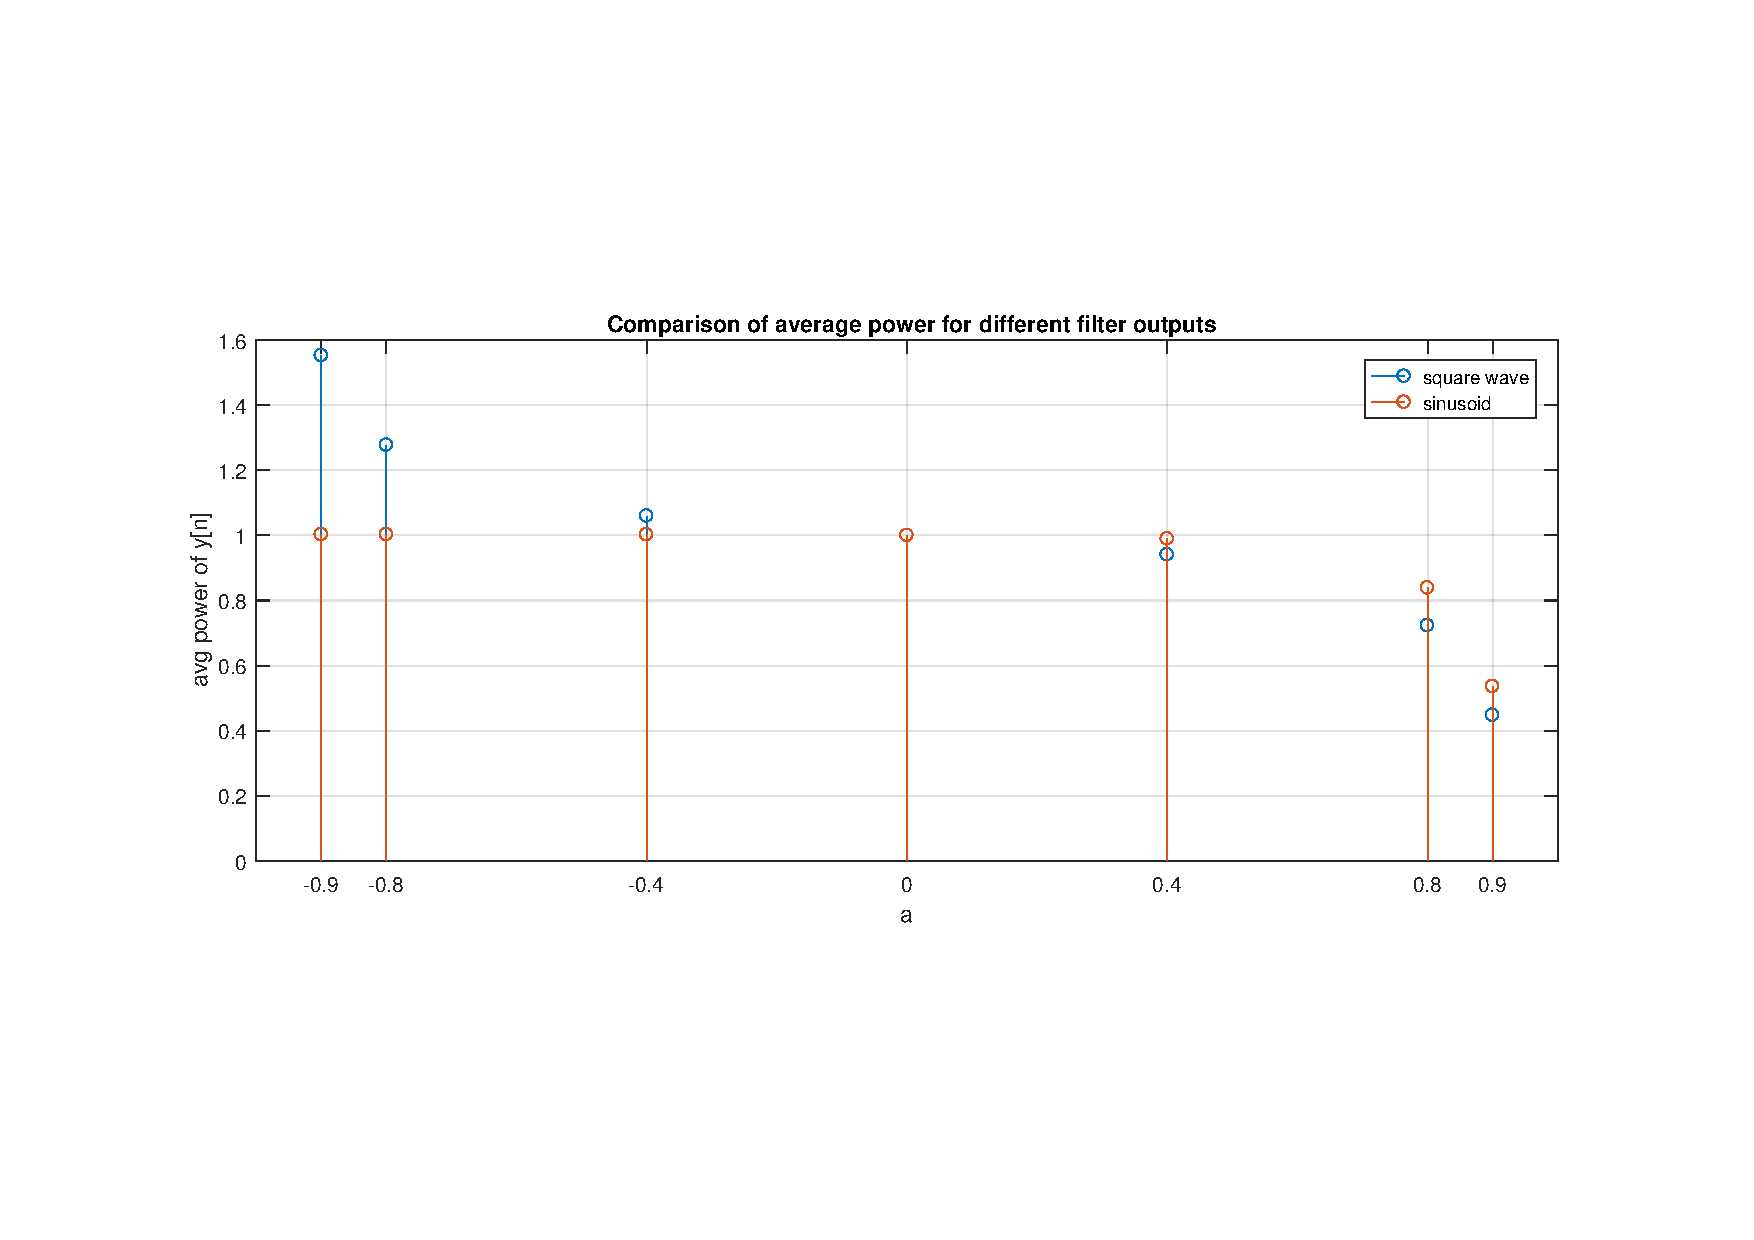
\includegraphics[trim={2.5cm 5cm 2.5cm 5cm}, clip, width=0.7\linewidth]{power}
	\caption{Average power of the outputs with different values of $a$}
	\label{fig:t1_power}
\end{figure}

\begin{figure} [H]
	\centering
	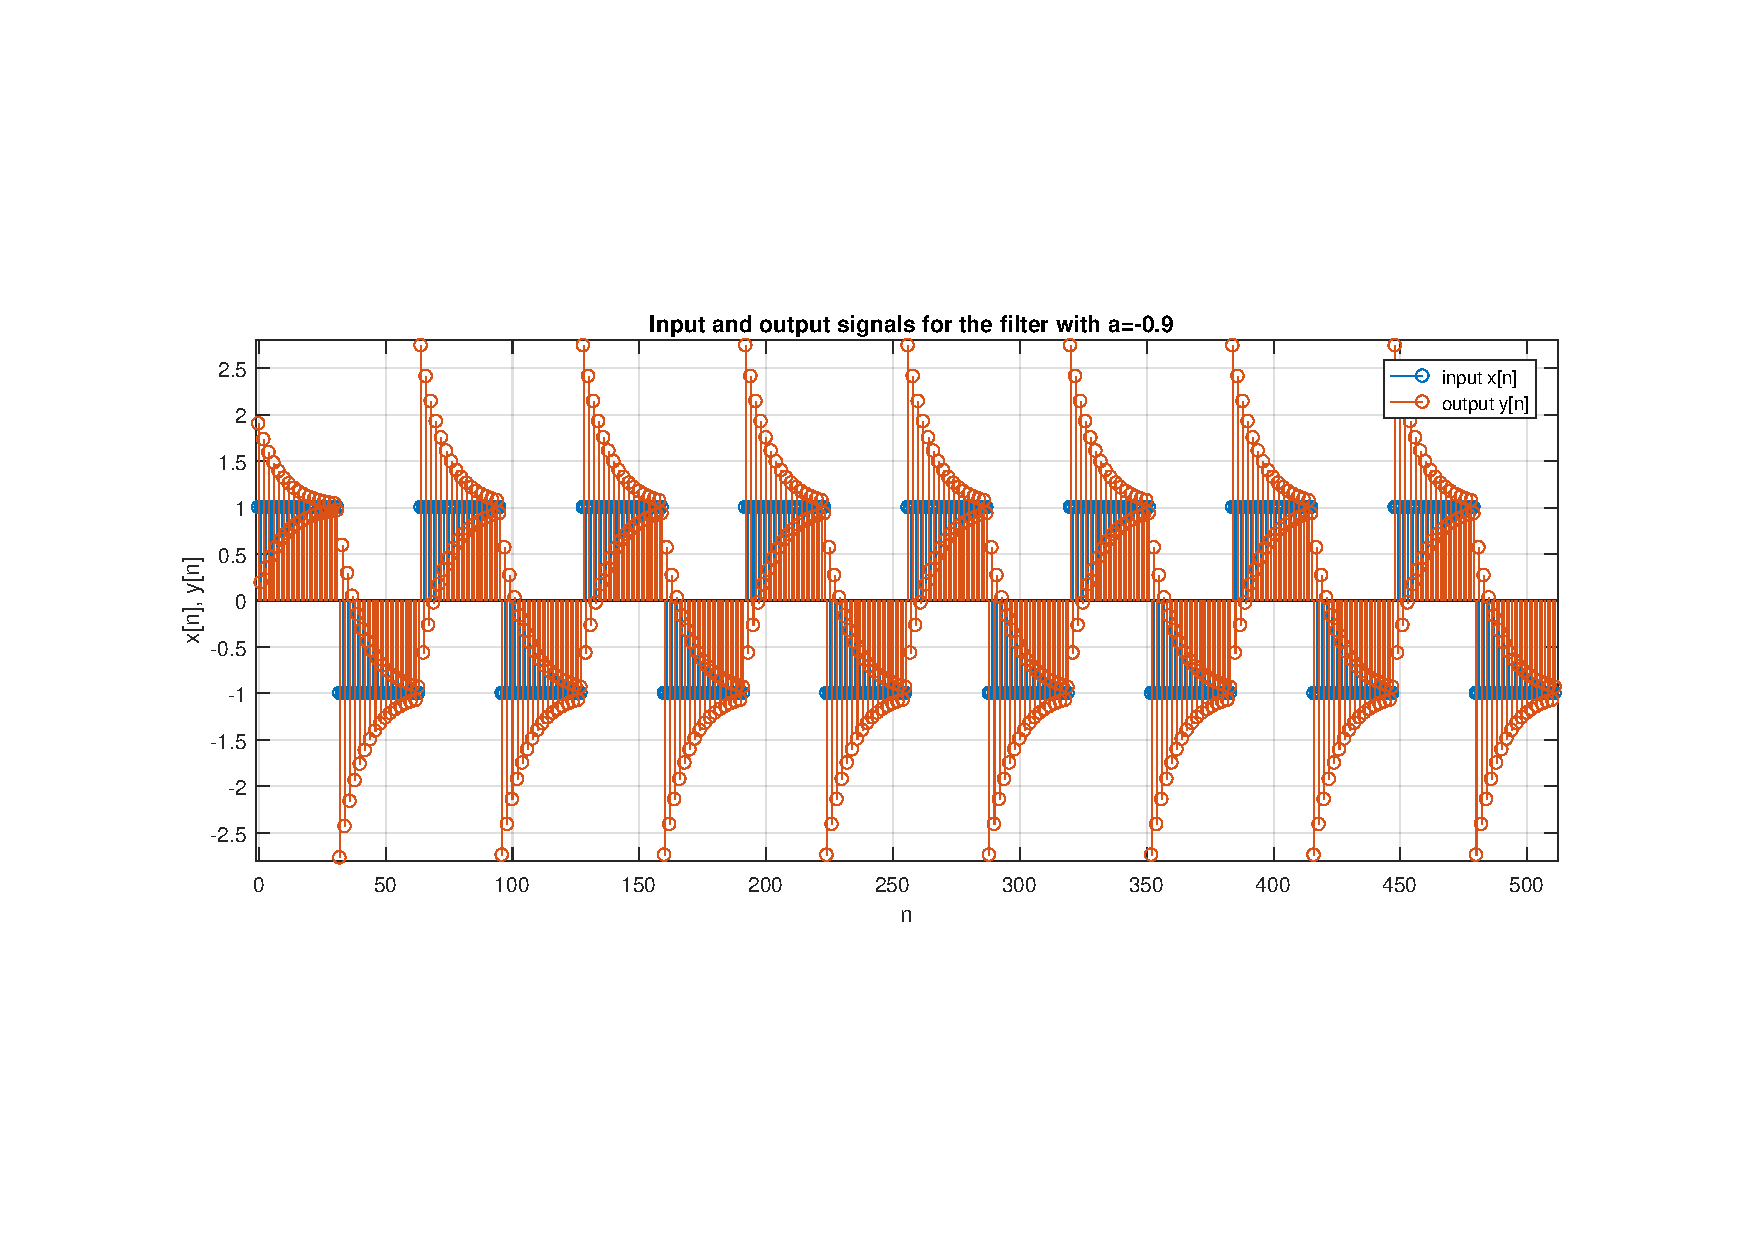
\includegraphics[trim={2.5cm 5cm 2.5cm 5cm}, clip, width=0.75\linewidth]{io_sw_1}
	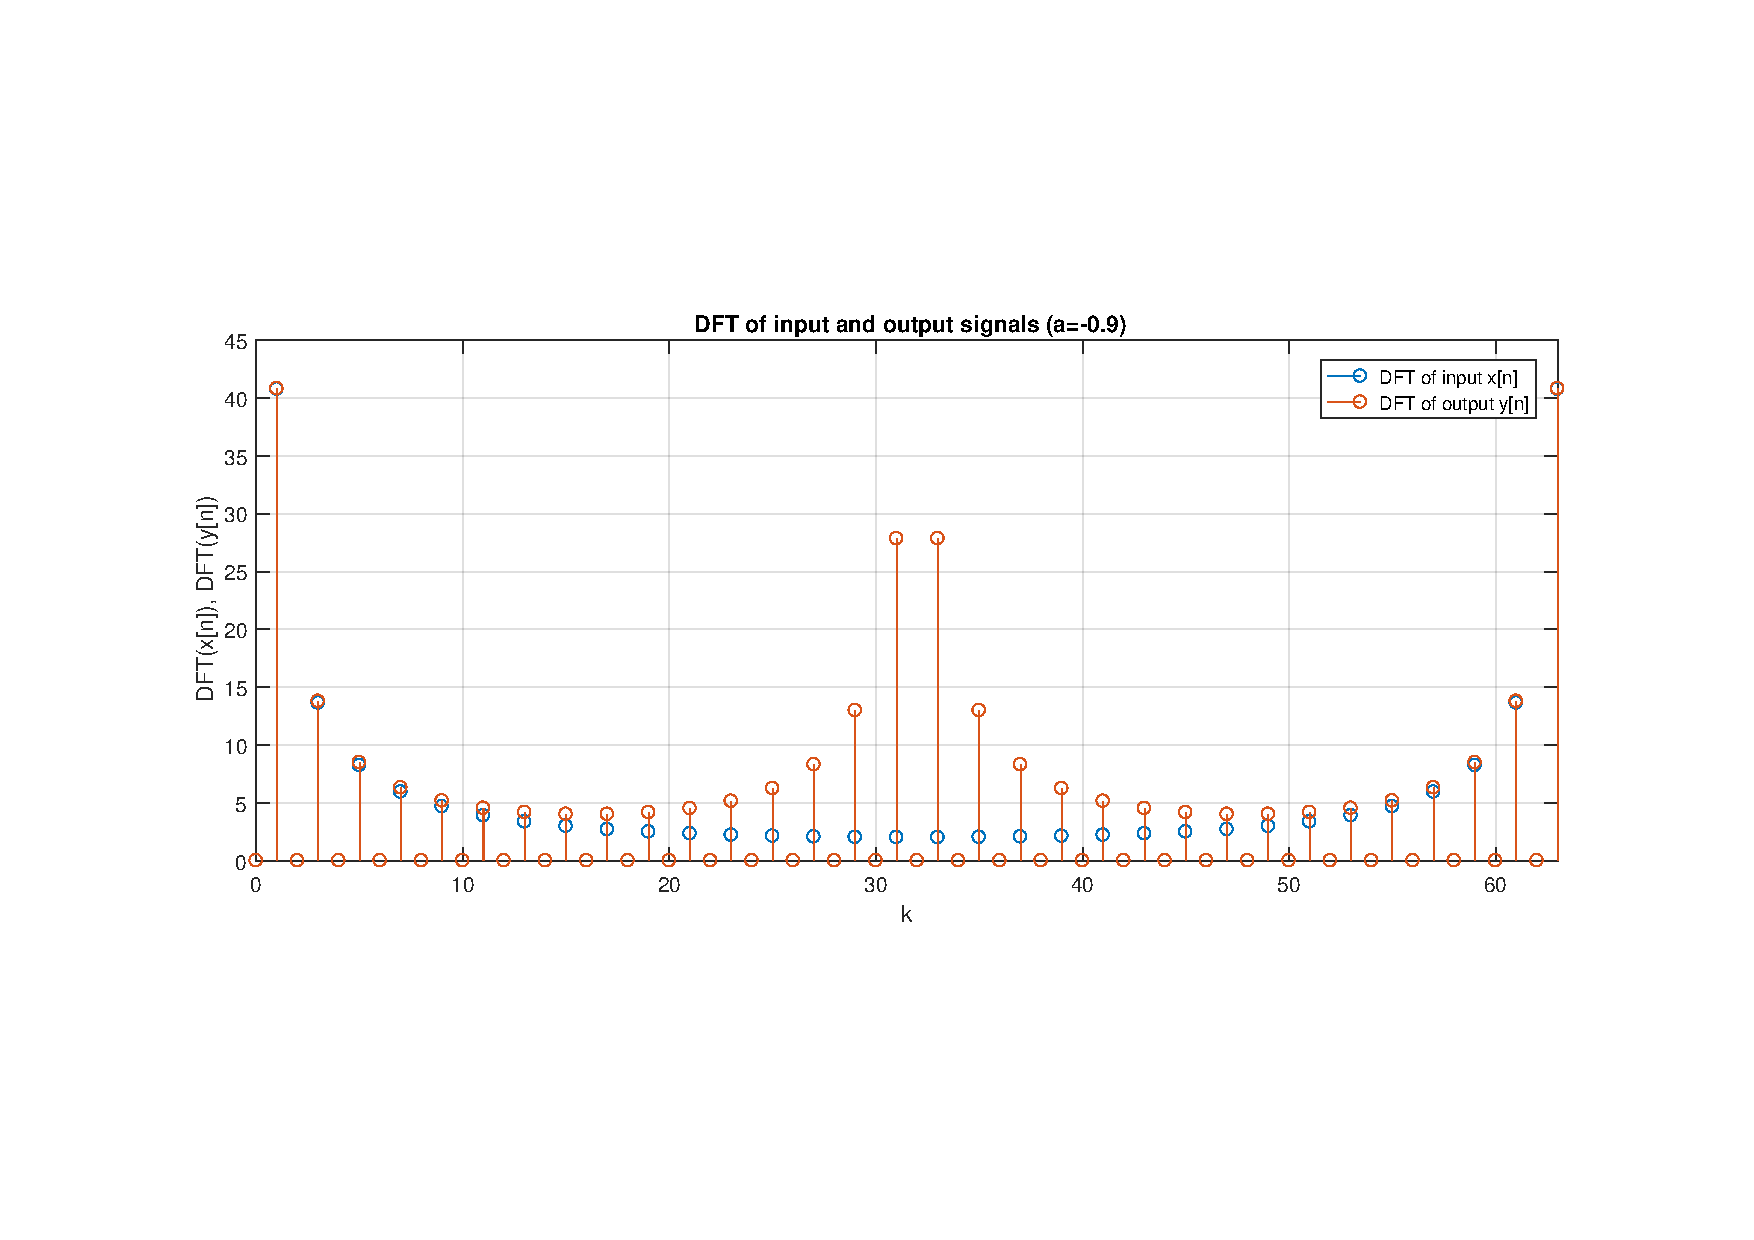
\includegraphics[trim={2.5cm 5cm 2.5cm 5cm}, clip, width=0.75\linewidth]{dft_sw_1}
	\caption{Input and output of the filter and their DFT, square wave input, $a=-0.9$ - alternating peaks on the rising edge of the square wave can be noticed, HF are amplified}
	\label{fig:t1_io_sw_1}
\end{figure}
\begin{figure} [H]
	\centering
	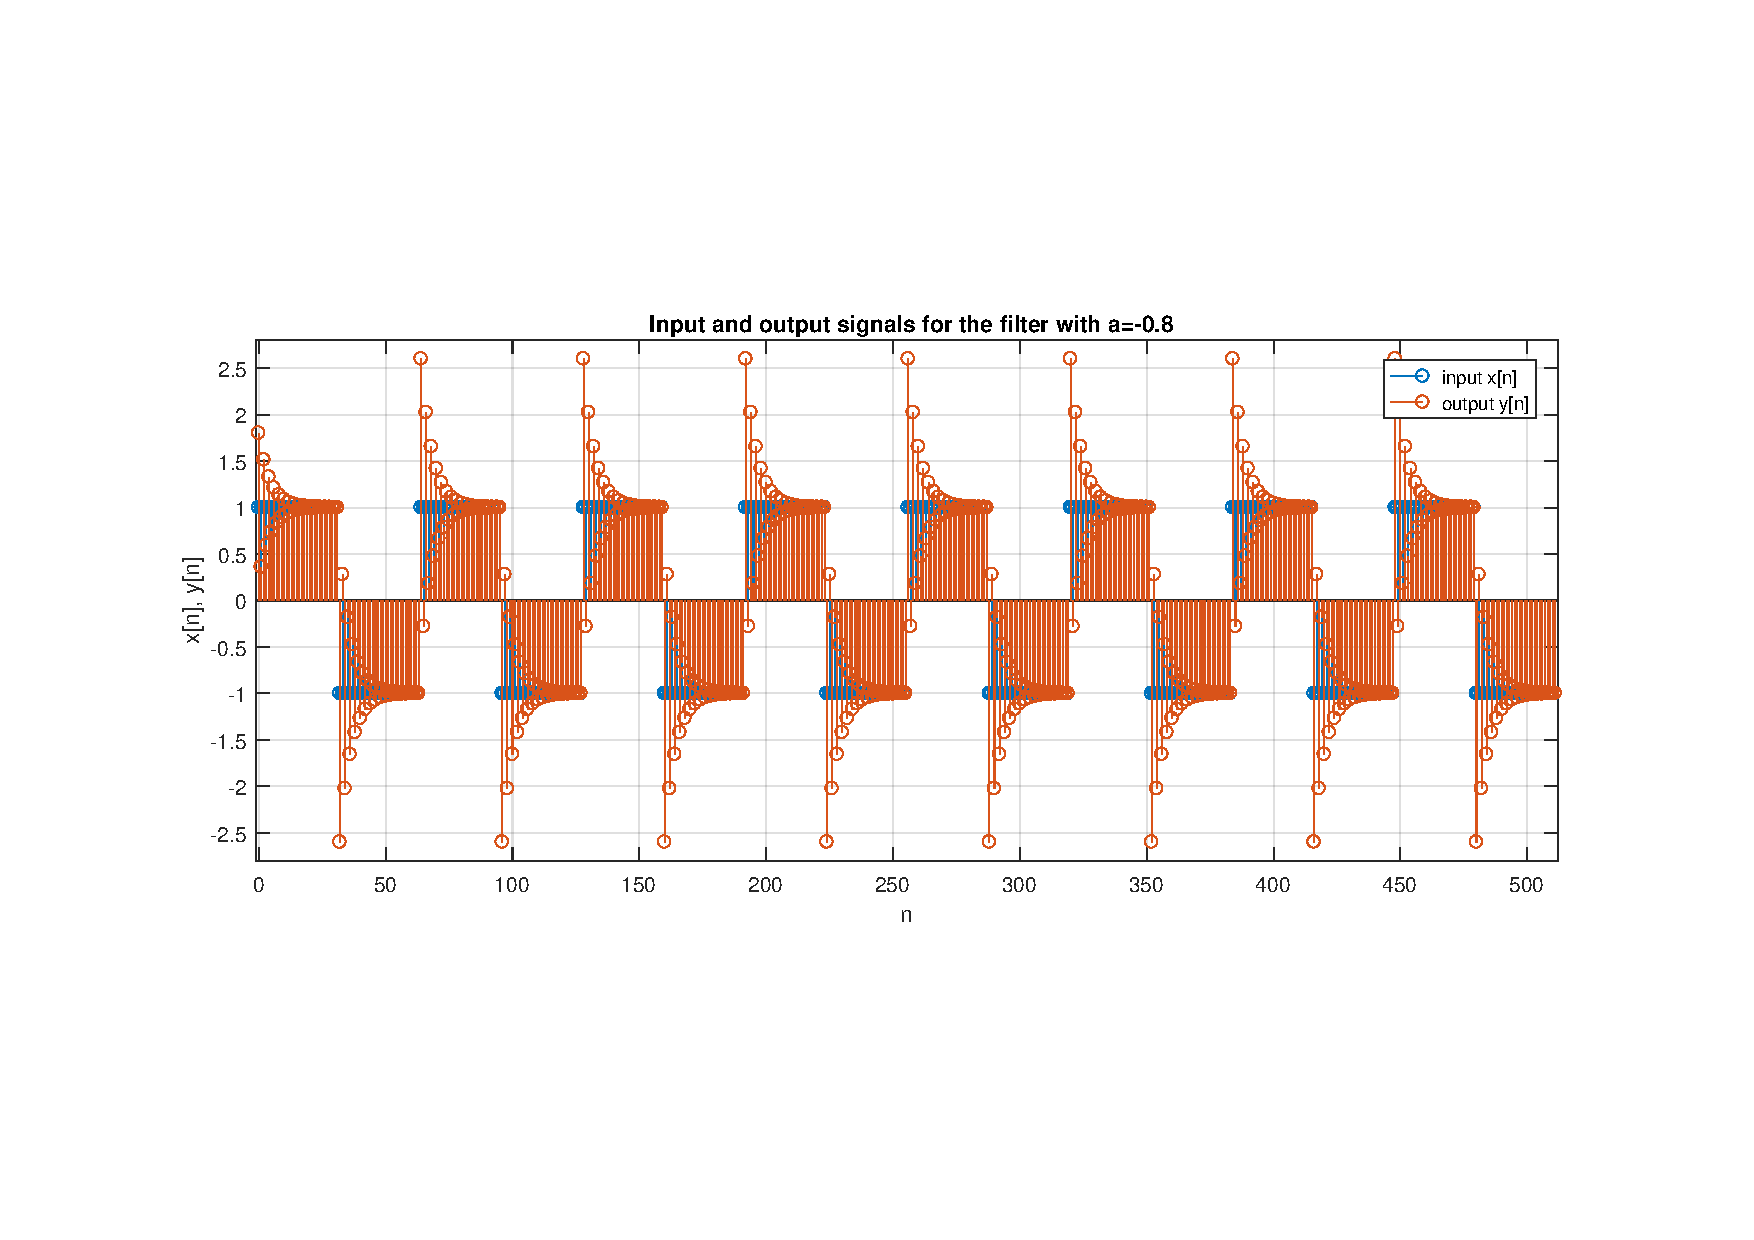
\includegraphics[trim={2.5cm 5cm 2.5cm 5cm}, clip, width=0.75\linewidth]{io_sw_2}
	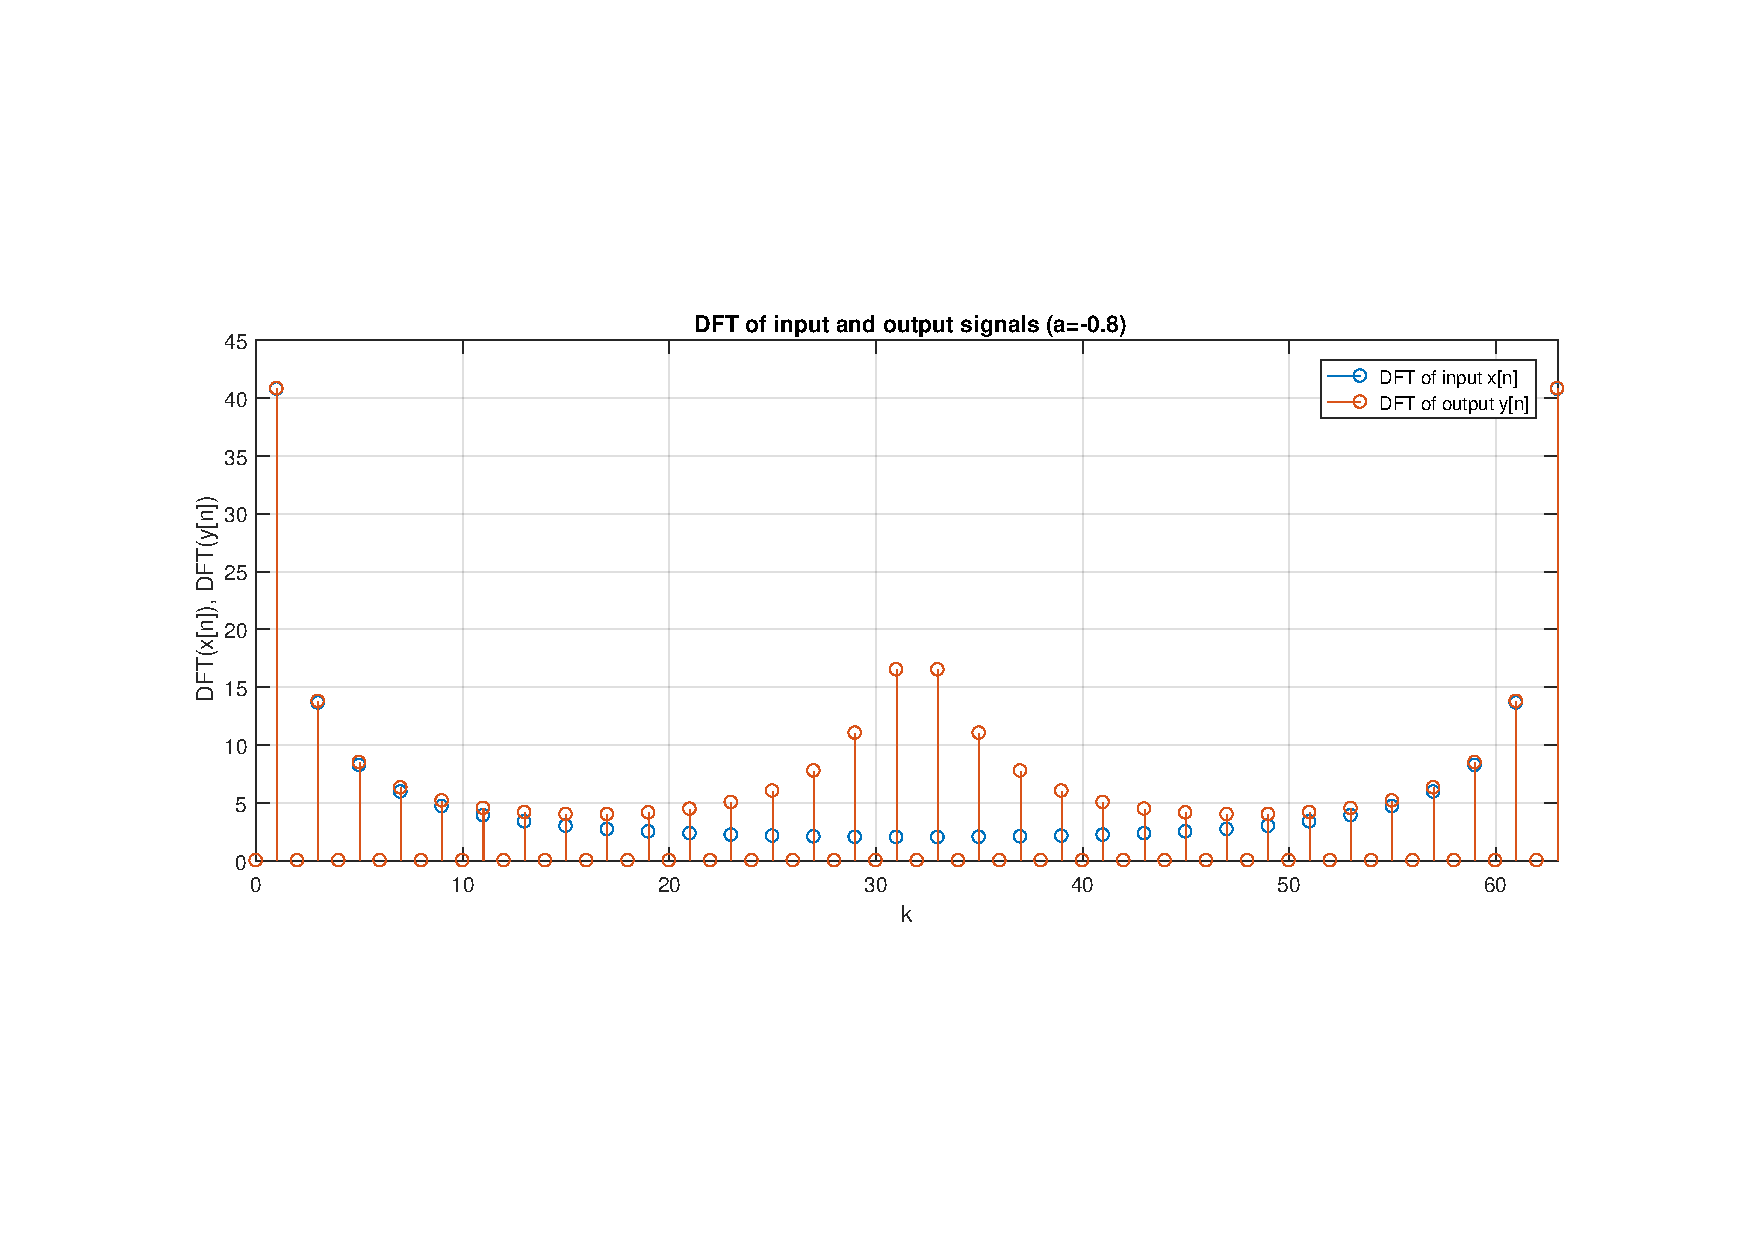
\includegraphics[trim={2.5cm 5cm 2.5cm 5cm}, clip, width=0.75\linewidth]{dft_sw_2}
	\caption{Input and output of the filter and their DFT, square wave input, $a=-0.8$}
	\label{fig:t1_io_sw_2}
\end{figure}
\begin{figure} [H]
	\centering
	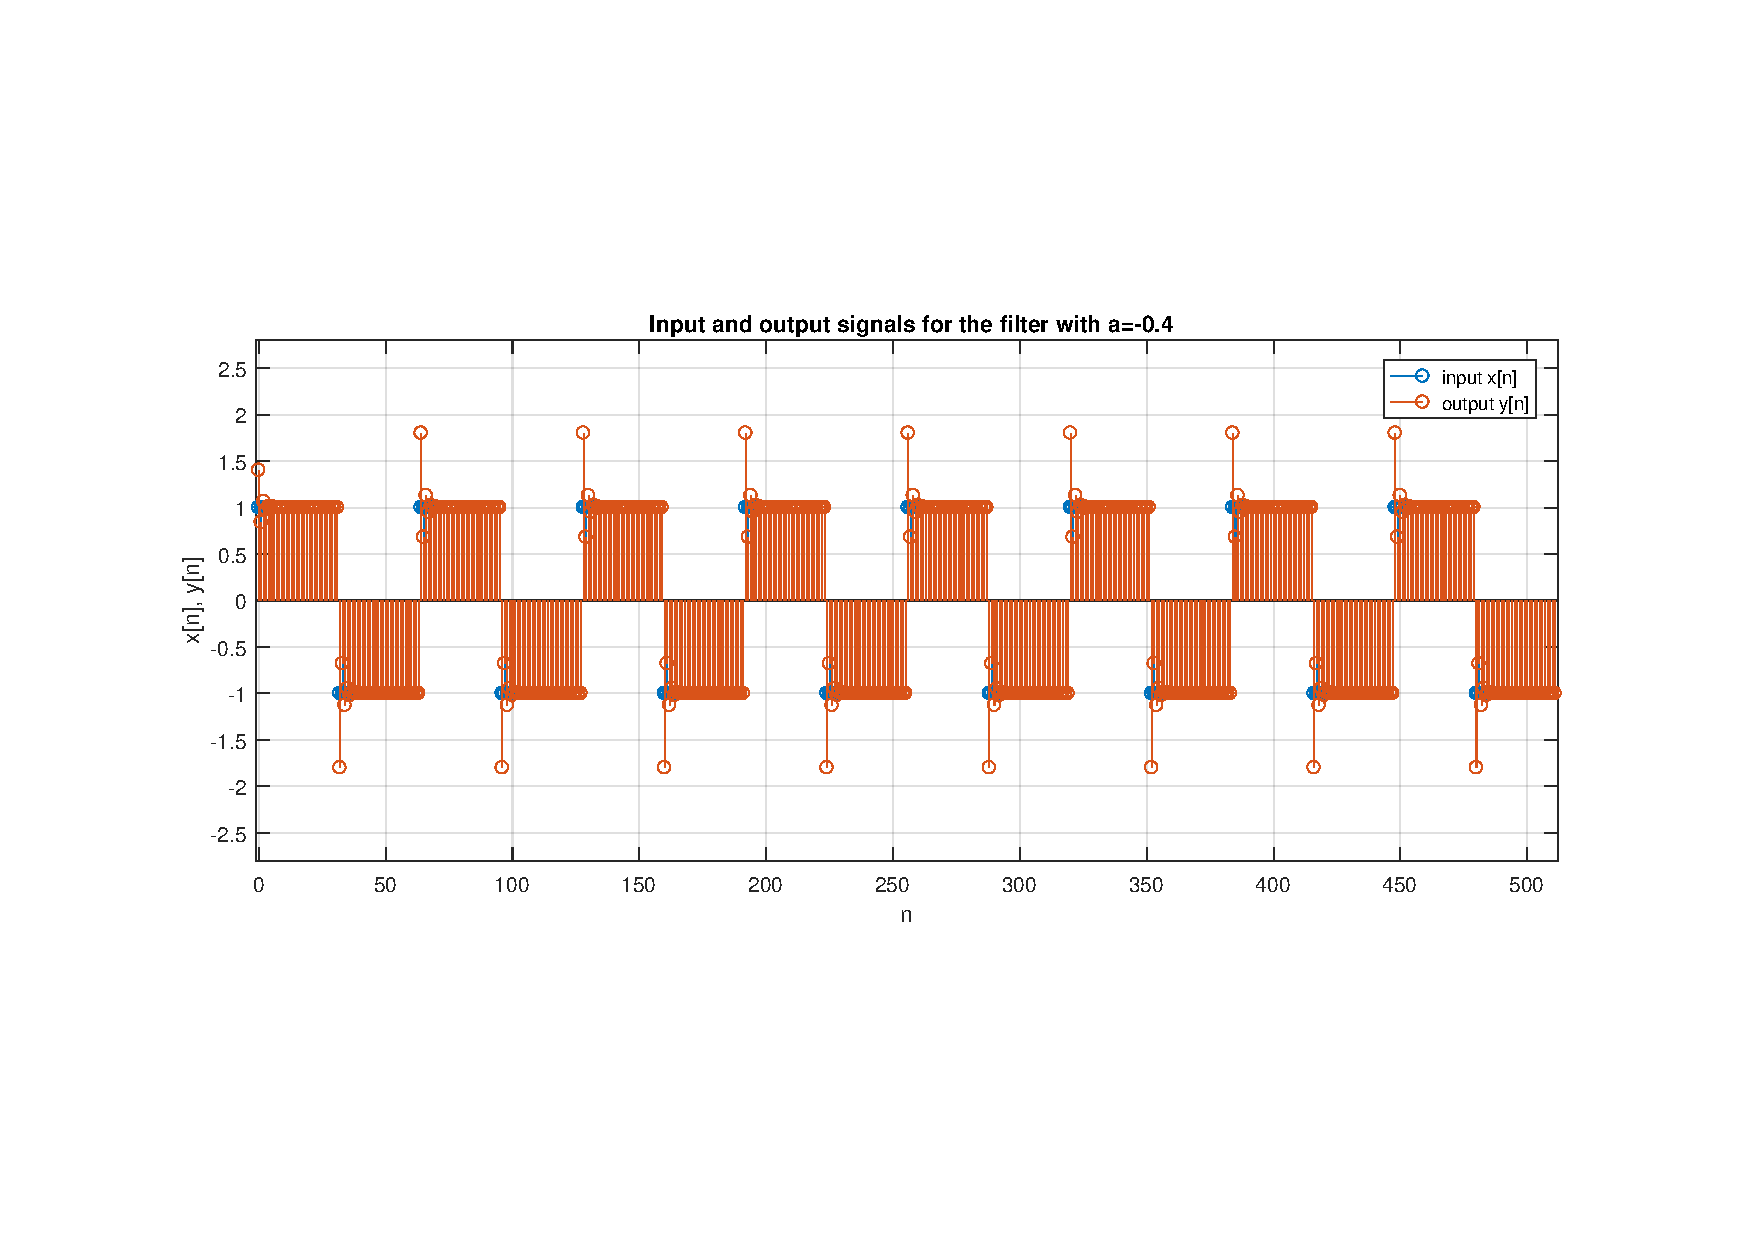
\includegraphics[trim={2.5cm 5cm 2.5cm 5cm}, clip, width=0.75\linewidth]{io_sw_3}
	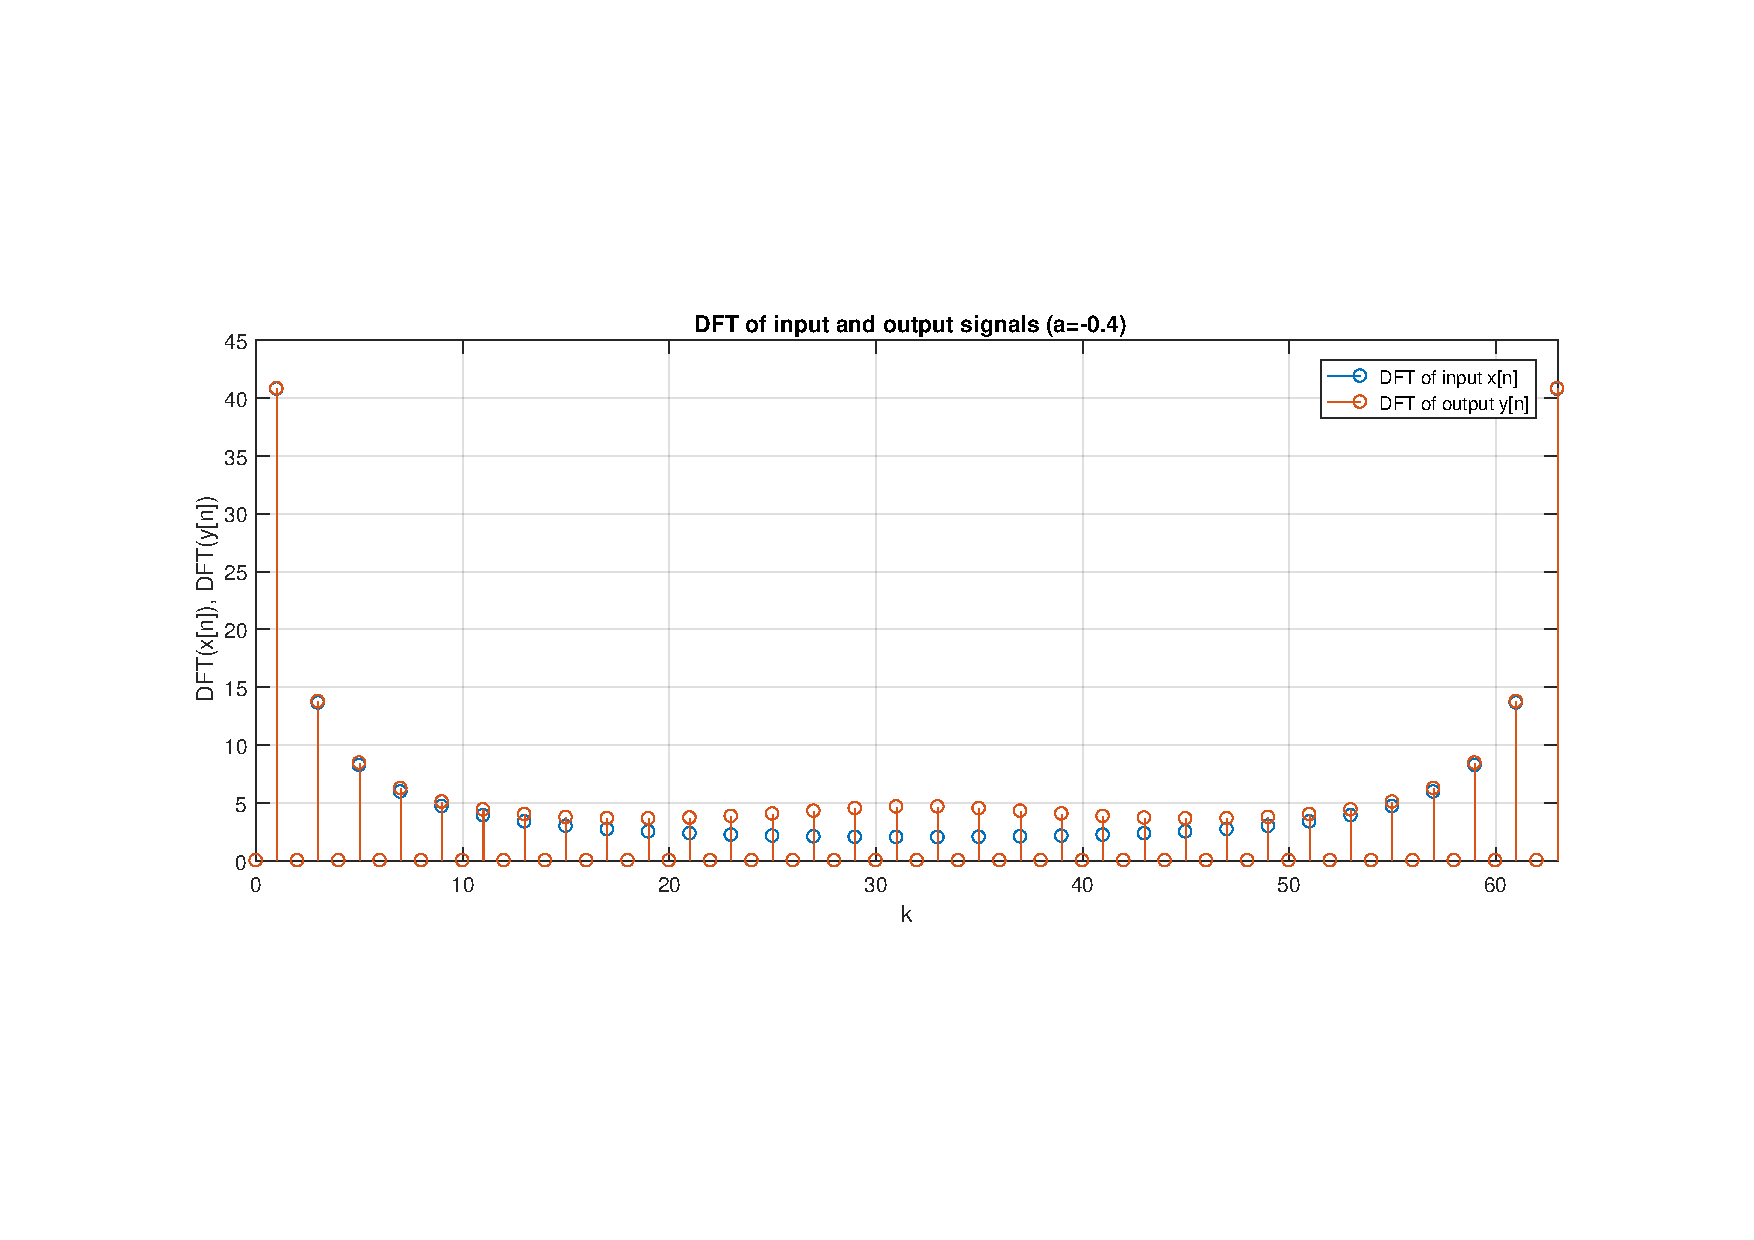
\includegraphics[trim={2.5cm 5cm 2.5cm 5cm}, clip, width=0.75\linewidth]{dft_sw_3}
	\caption{Input and output of the filter and their DFT, square wave input, $a=-0.4$}
	\label{fig:t1_io_sw_3}
\end{figure}
\begin{figure} [H]
	\centering
	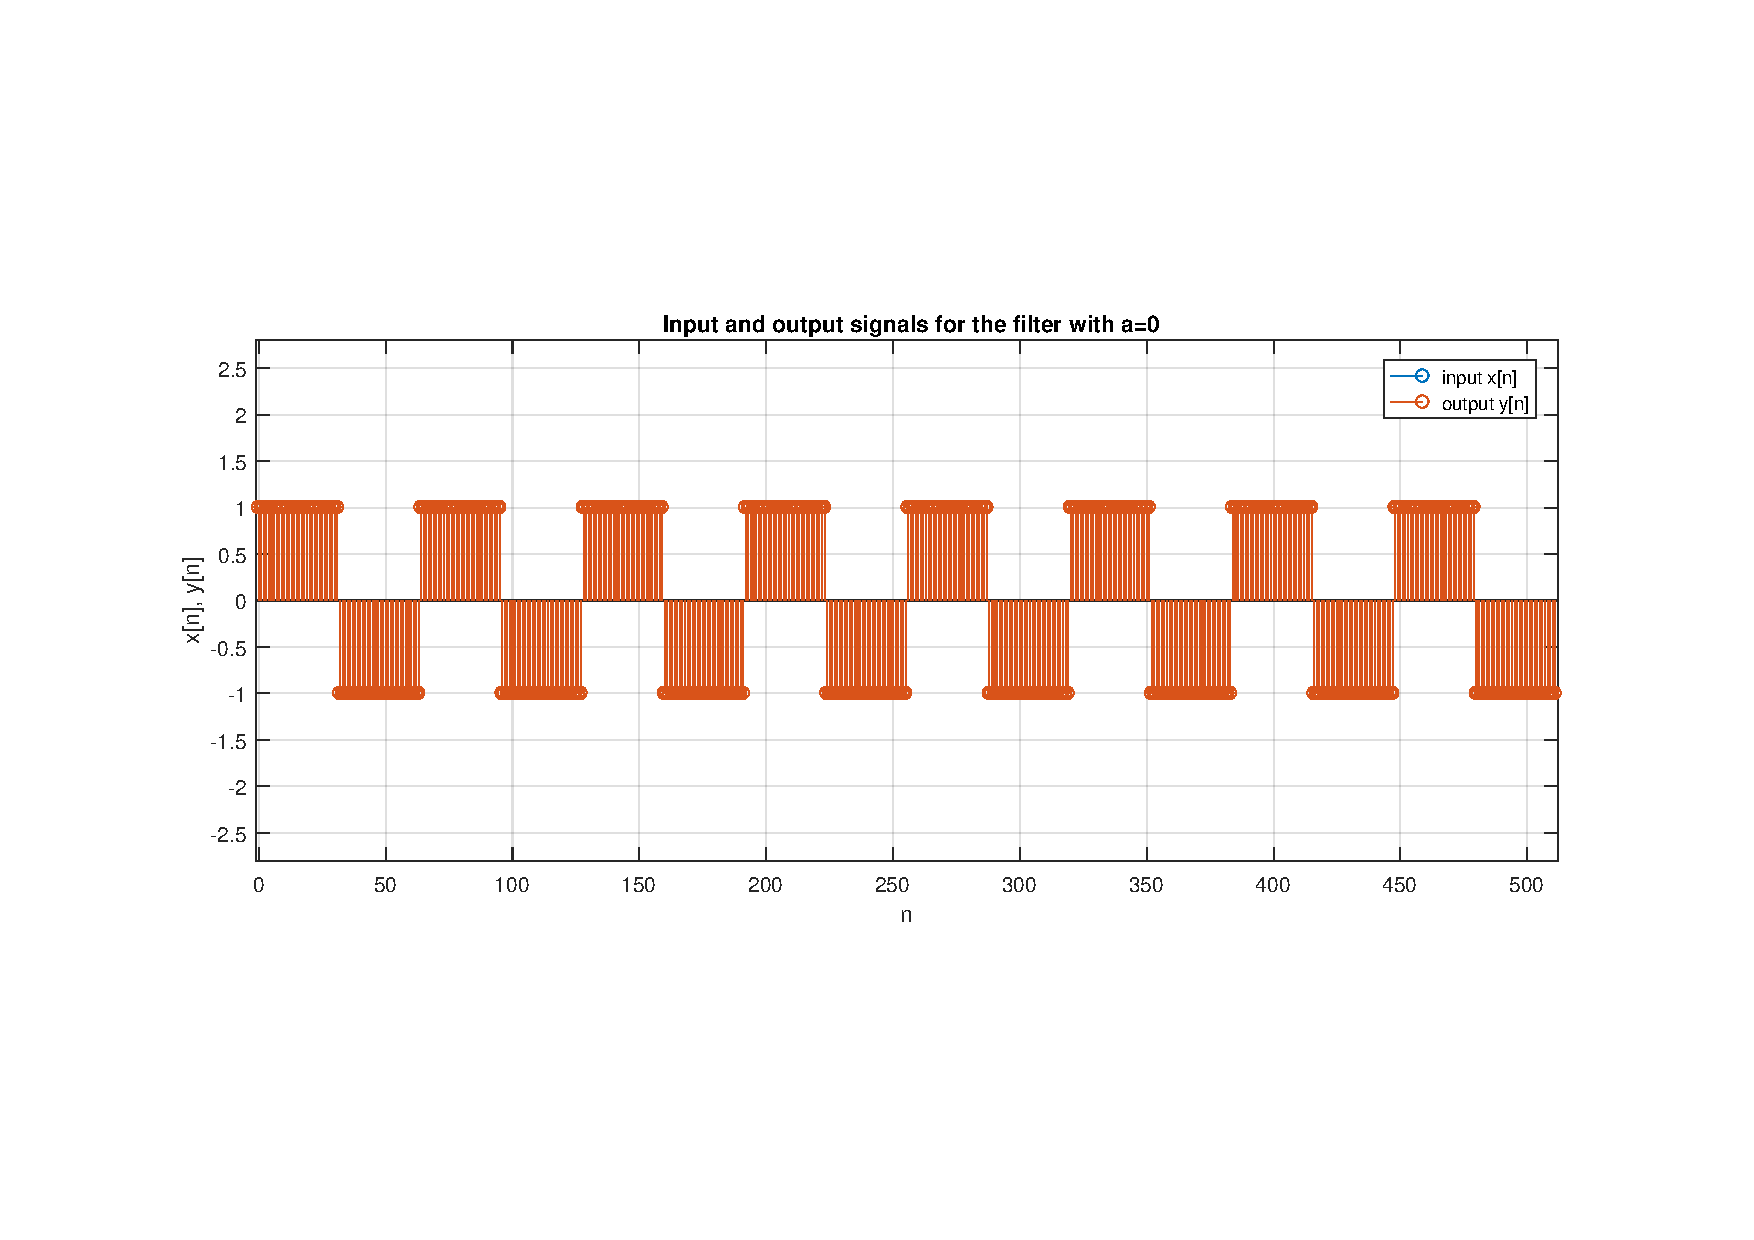
\includegraphics[trim={2.5cm 5cm 2.5cm 5cm}, clip, width=0.75\linewidth]{io_sw_4}
	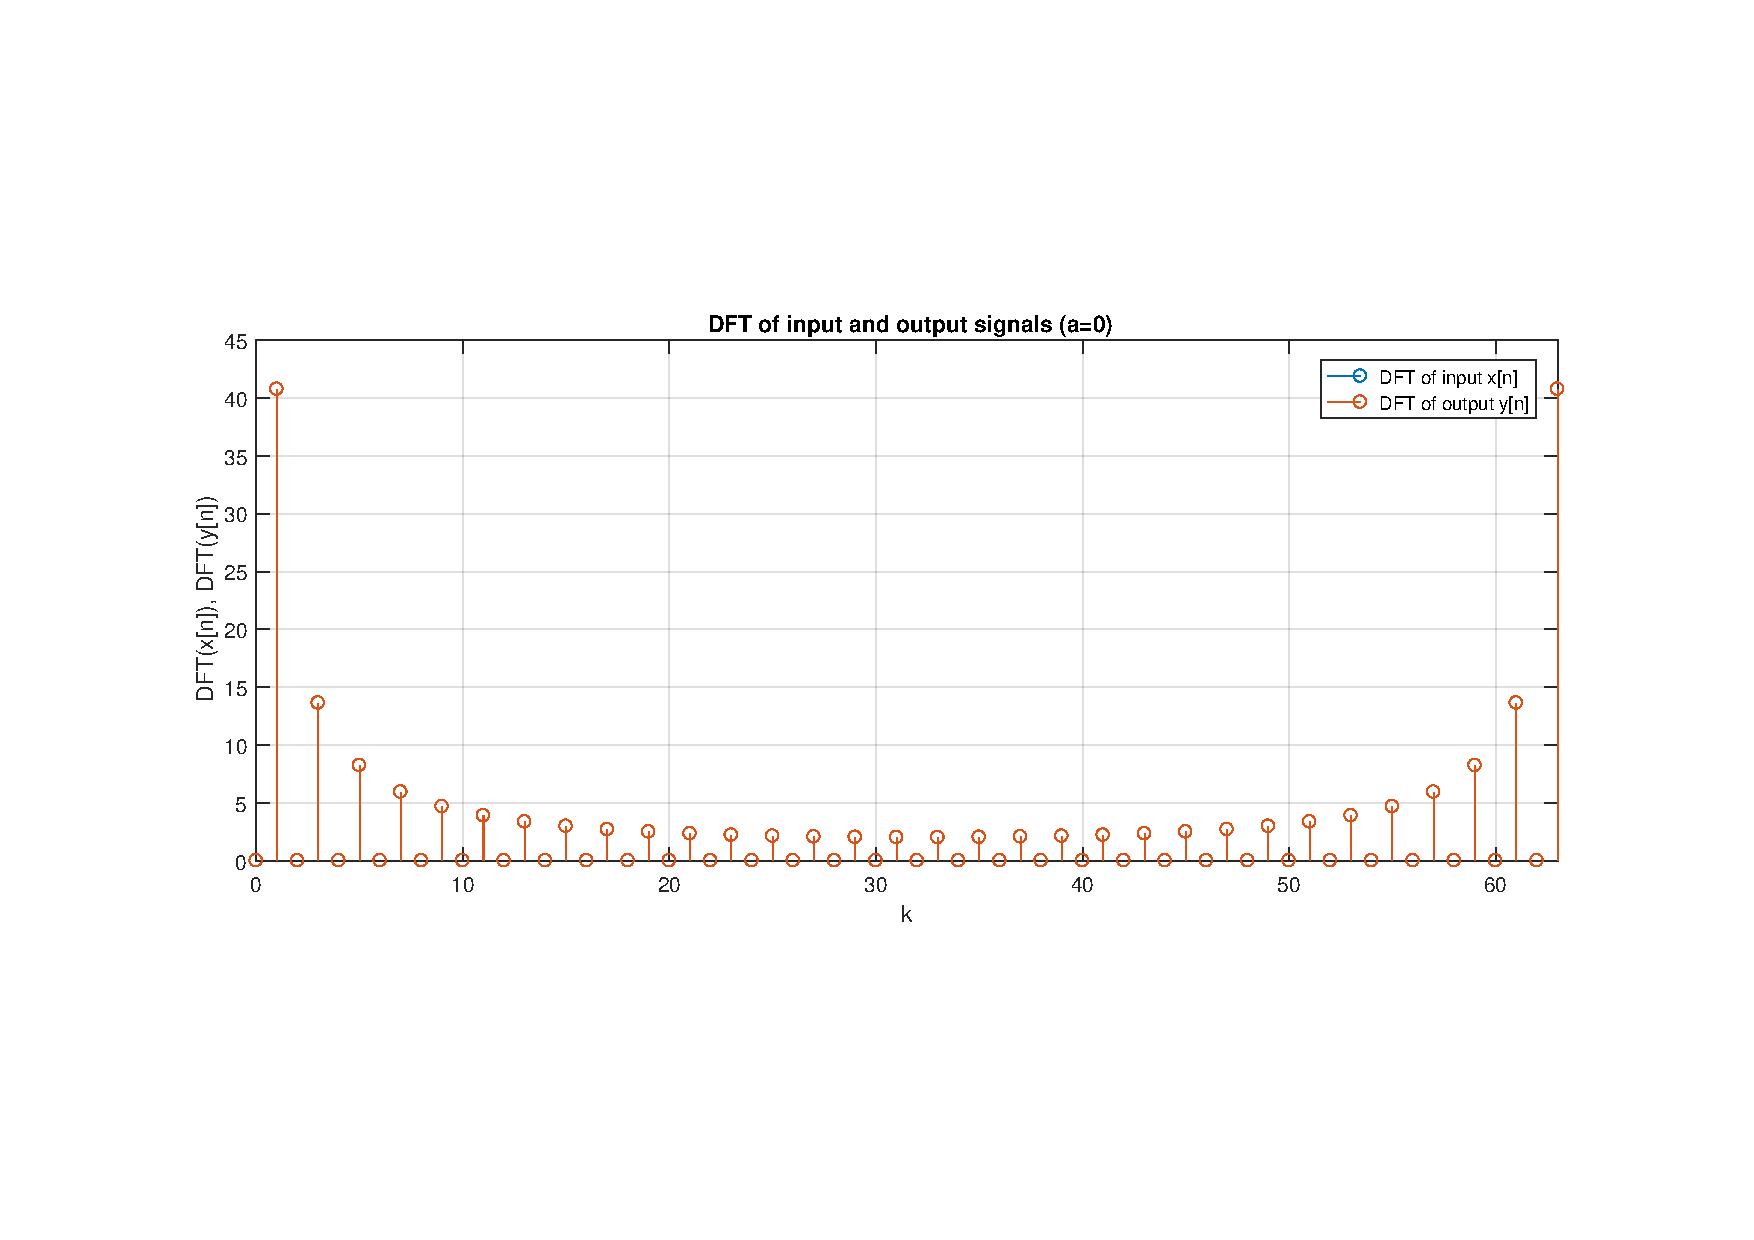
\includegraphics[trim={2.5cm 5cm 2.5cm 5cm}, clip, width=0.75\linewidth]{dft_sw_4}
	\caption{Input and output of the filter and their DFT, square wave input, $a=0$ - the output is equal to the input, unitary tf}
	\label{fig:t1_io_sw_4}
\end{figure}
\begin{figure} [H]
	\centering
	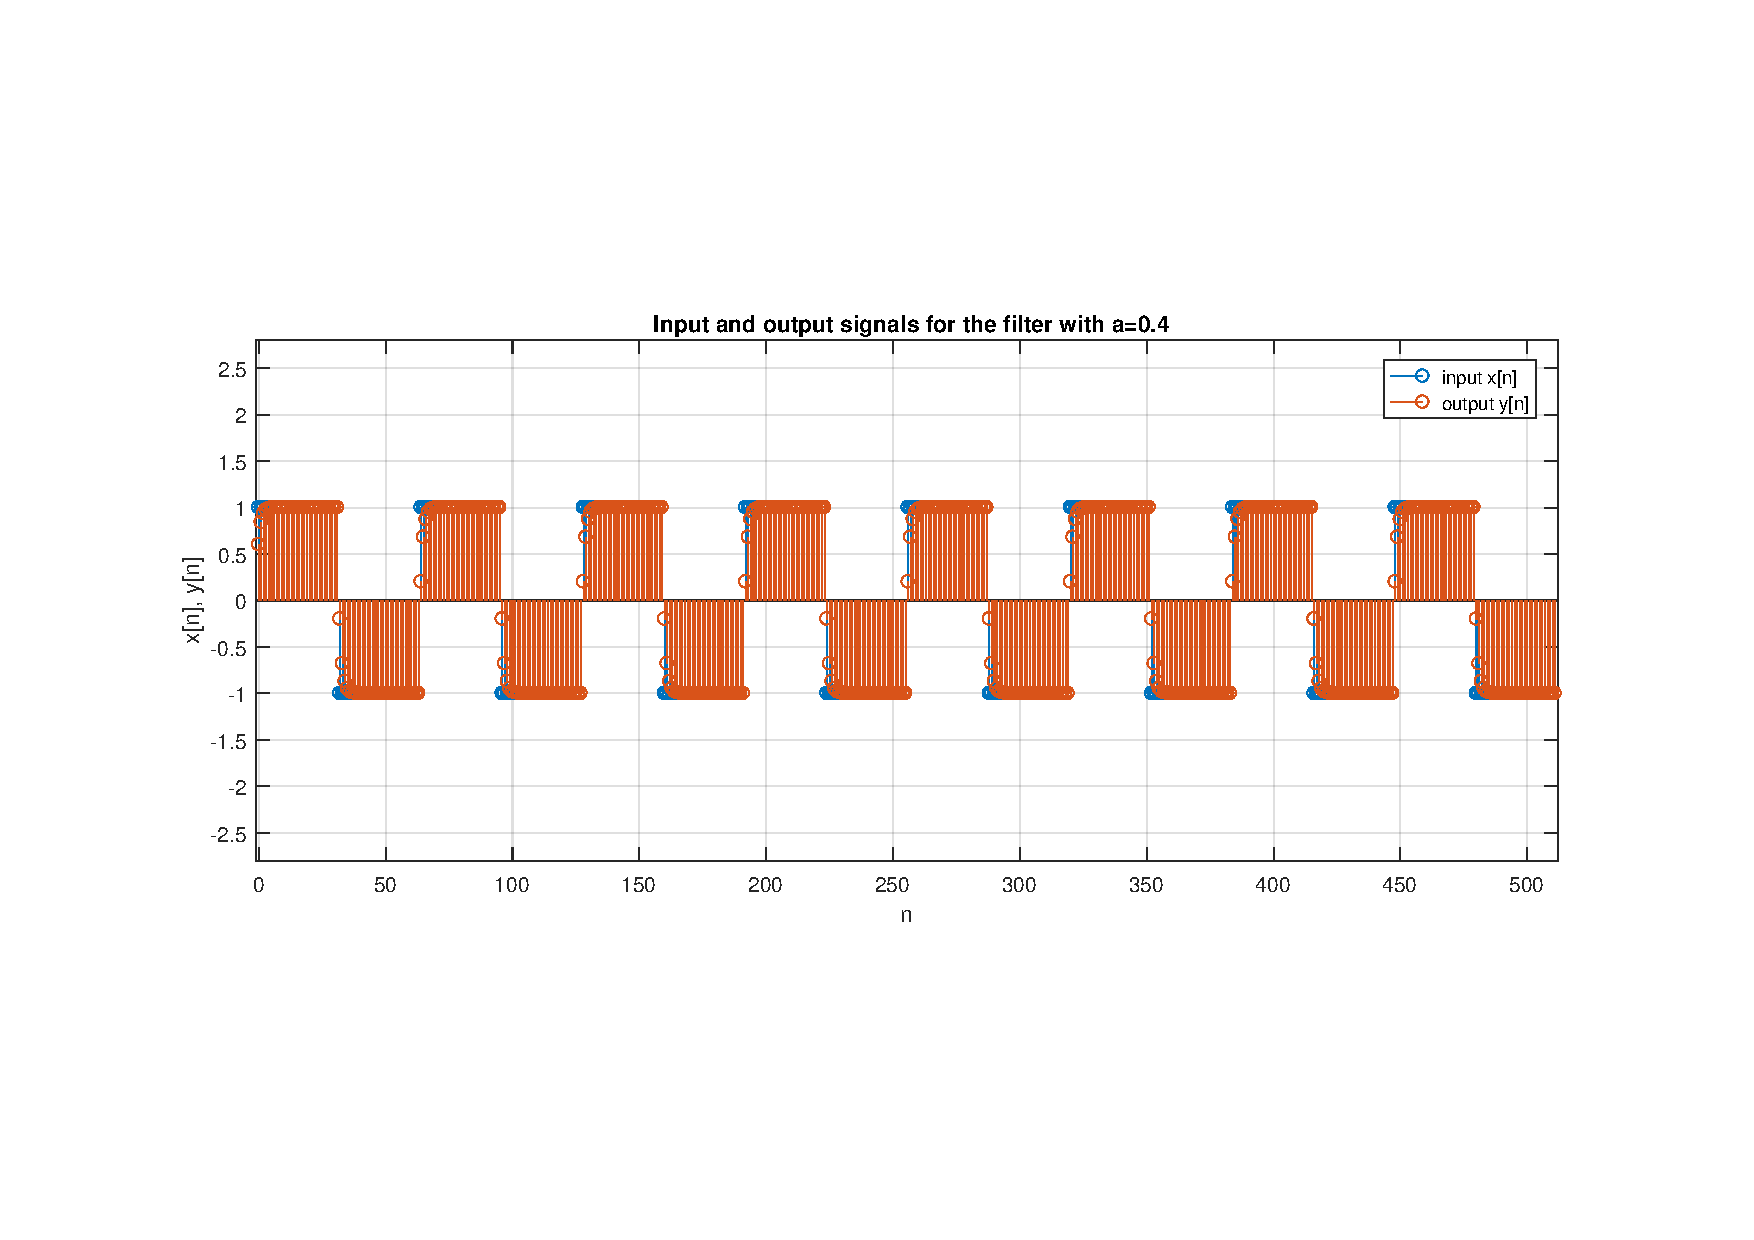
\includegraphics[trim={2.5cm 5cm 2.5cm 5cm}, clip, width=0.75\linewidth]{io_sw_5}
	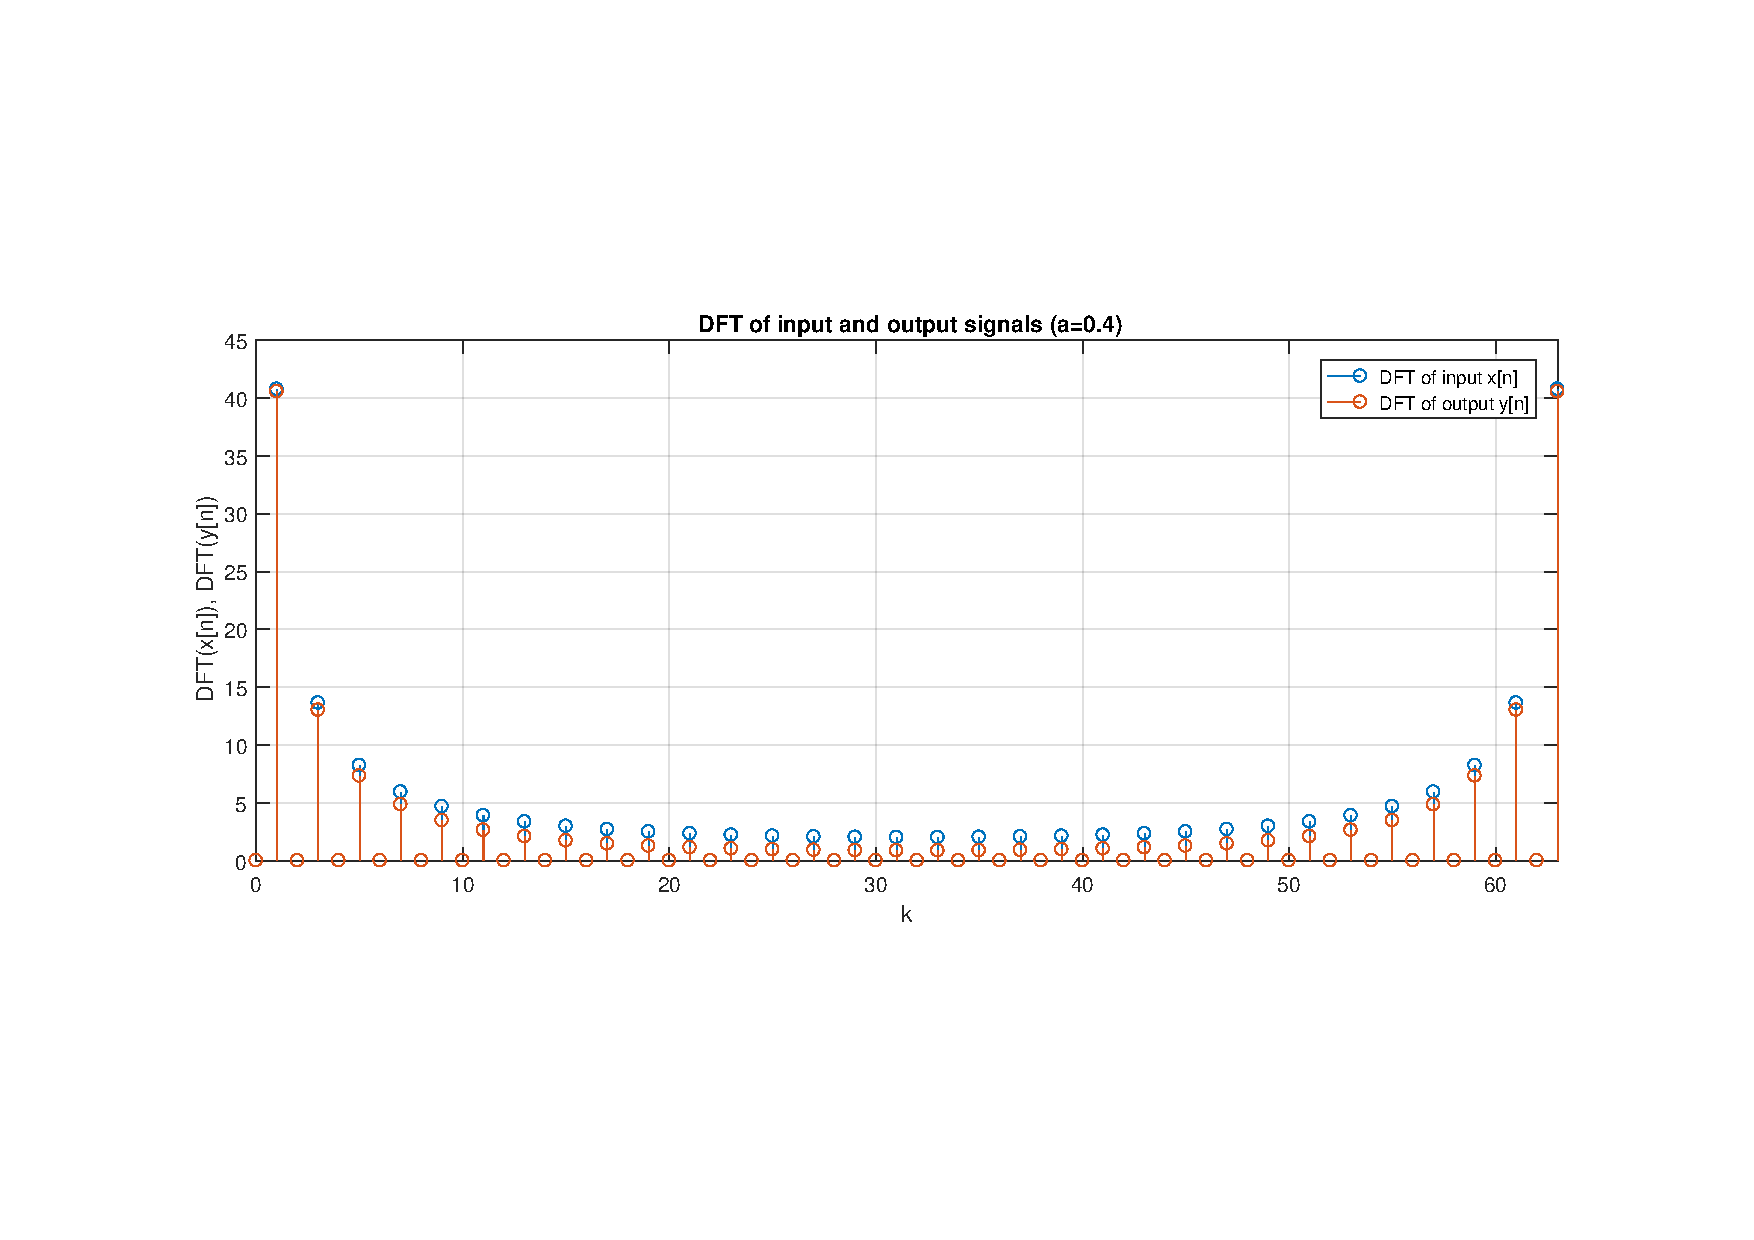
\includegraphics[trim={2.5cm 5cm 2.5cm 5cm}, clip, width=0.75\linewidth]{dft_sw_5}
	\caption{Input and output of the filter and their DFT, square wave input, $a=0.4$}
	\label{fig:t1_io_sw_5}
\end{figure}
\begin{figure} [H]
	\centering
	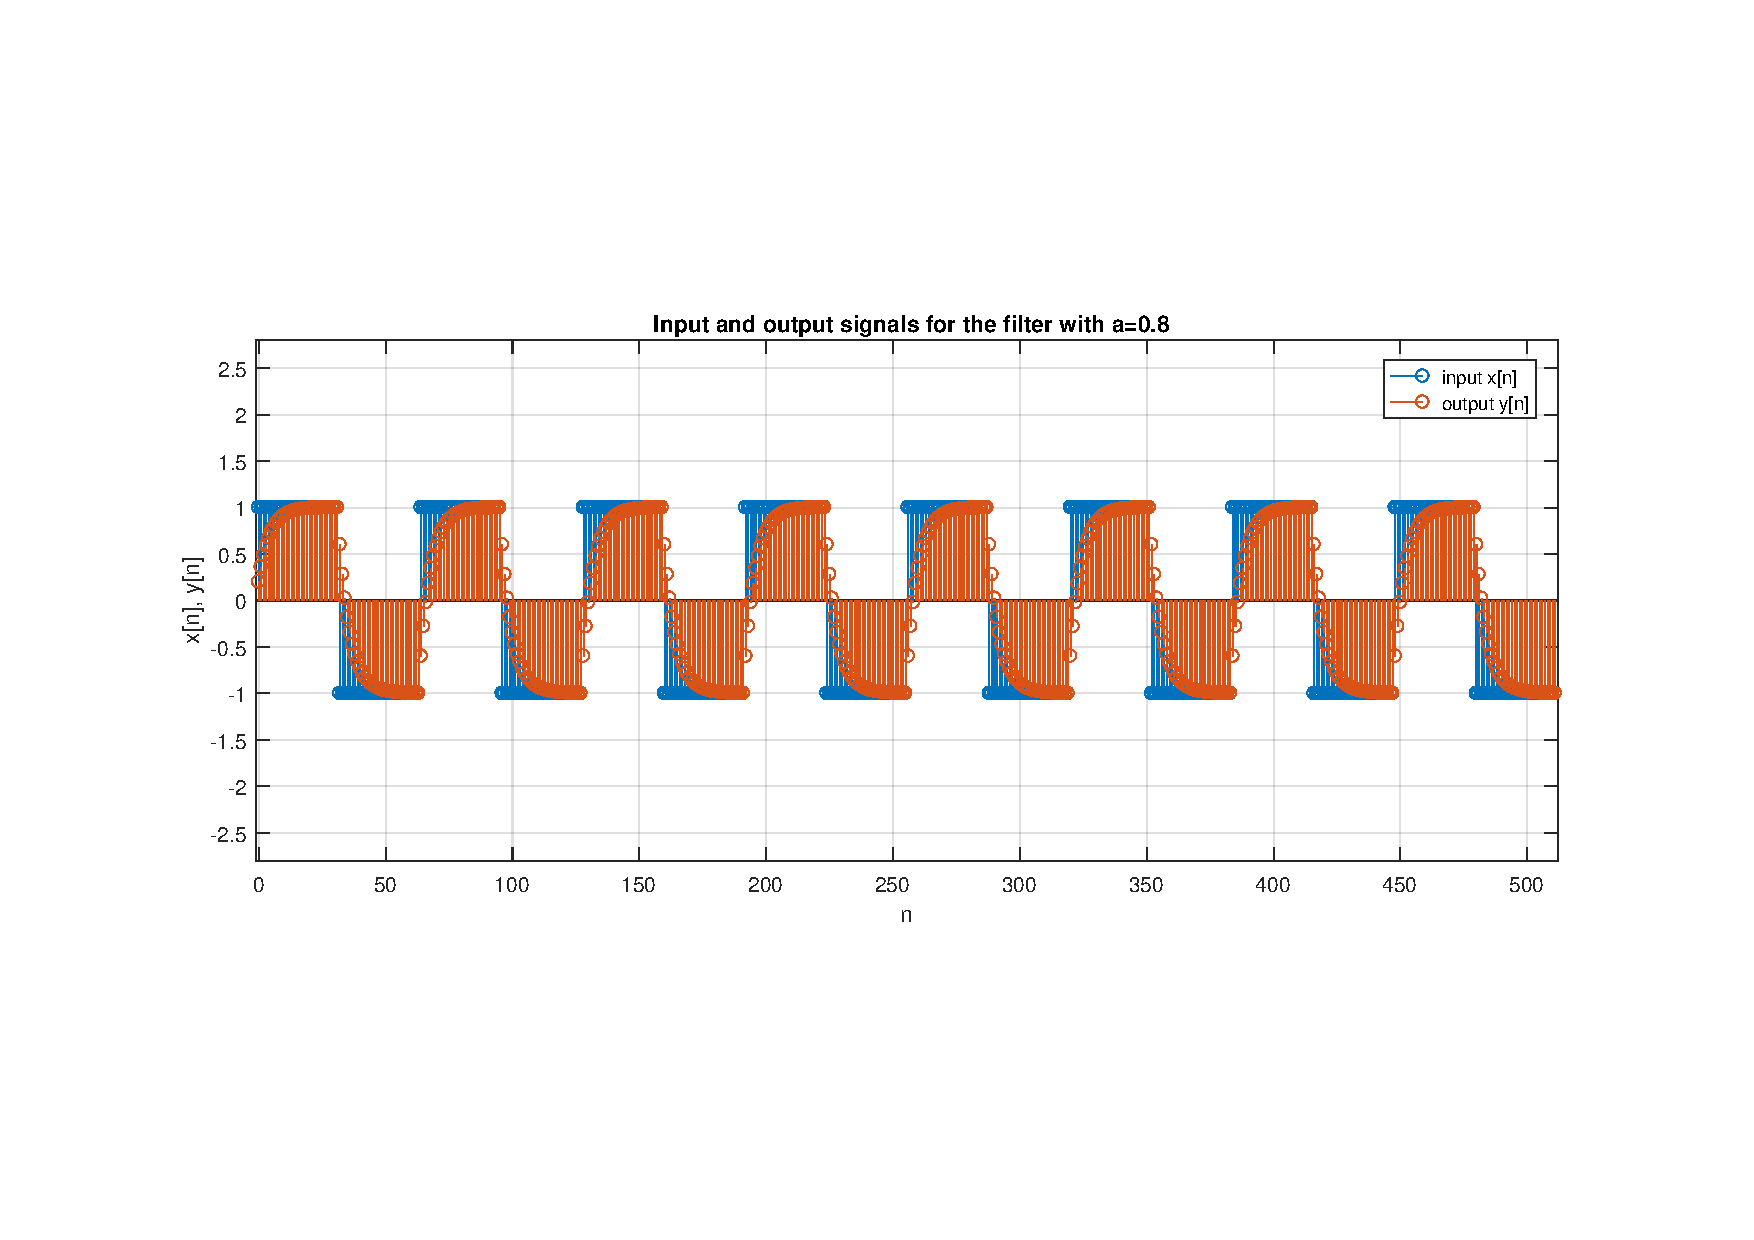
\includegraphics[trim={2.5cm 5cm 2.5cm 5cm}, clip, width=0.75\linewidth]{io_sw_6}
	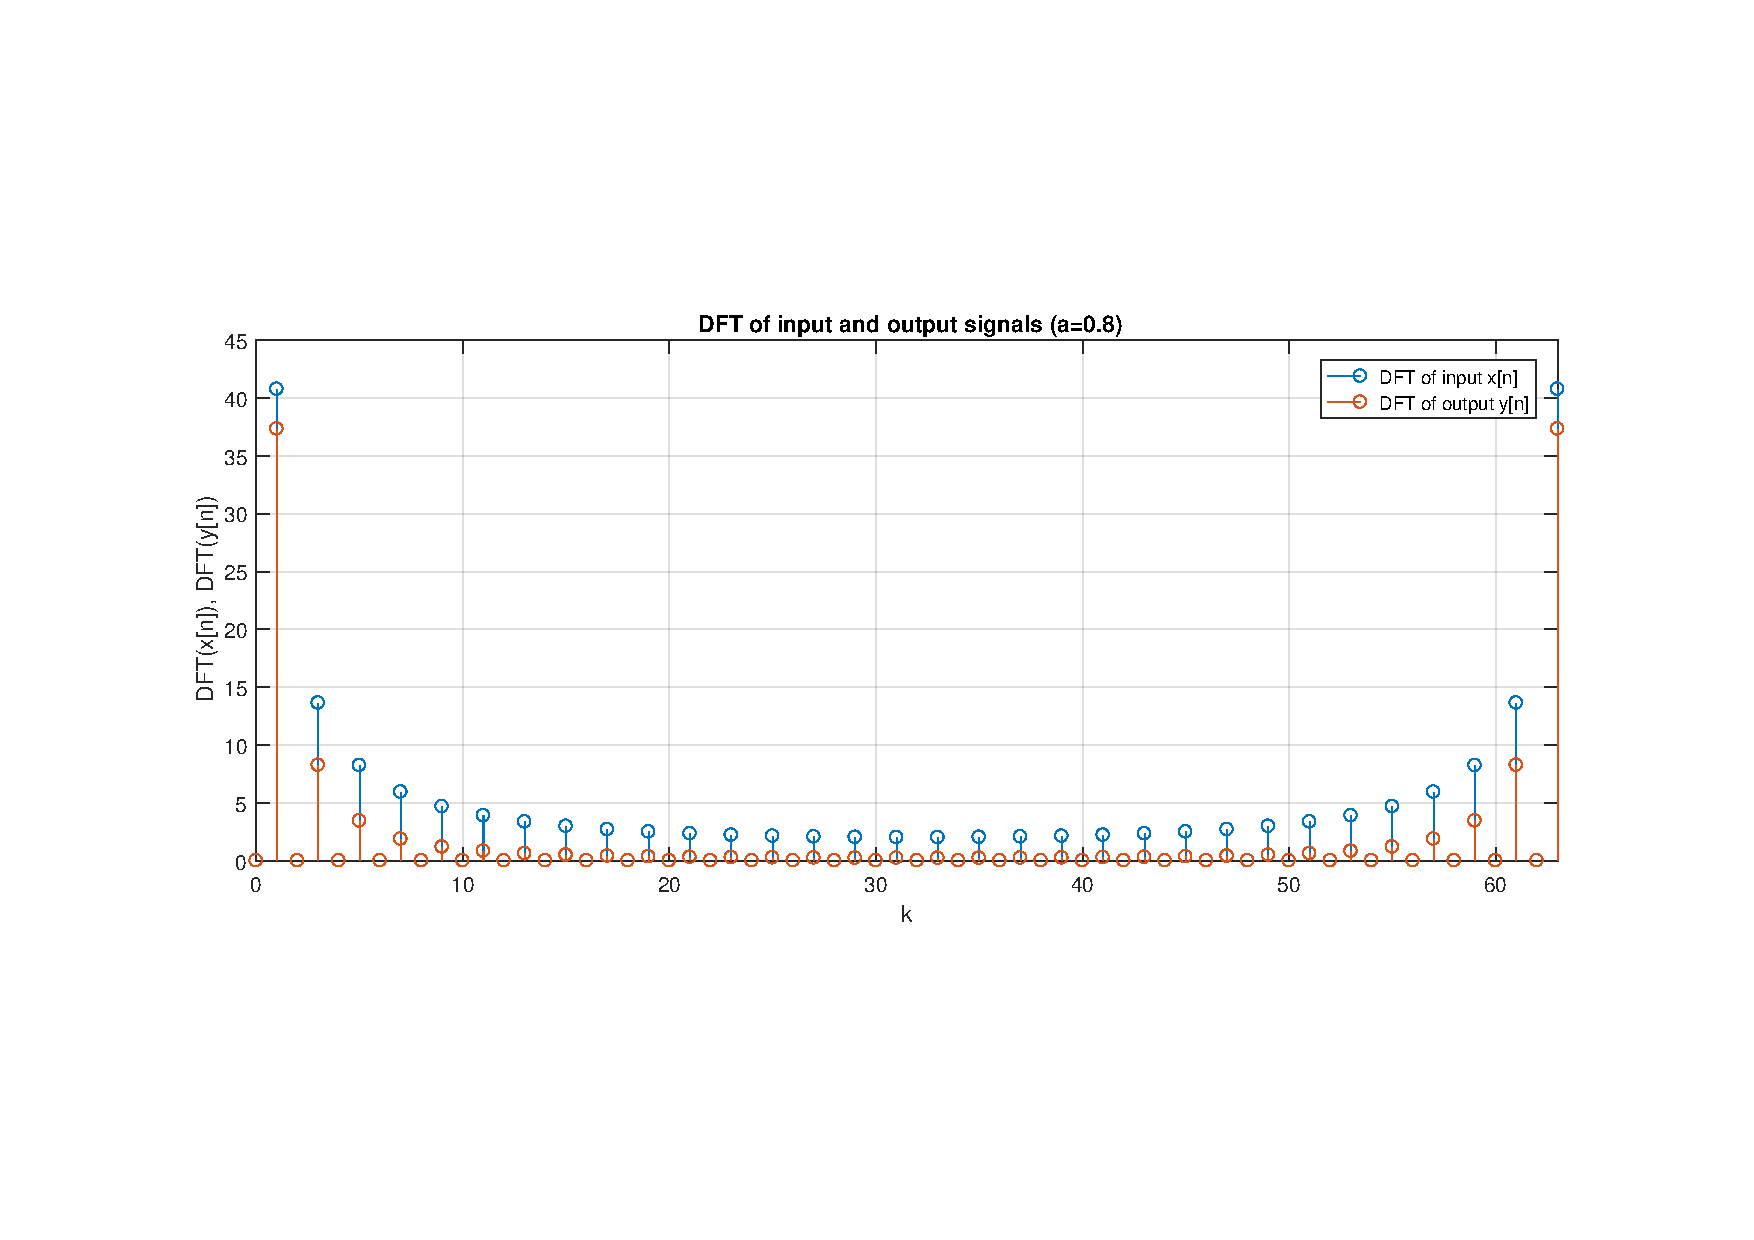
\includegraphics[trim={2.5cm 5cm 2.5cm 5cm}, clip, width=0.75\linewidth]{dft_sw_6}
	\caption{Input and output of the filter and their DFT, square wave input, $a=0.8$ - lowpass behavior, HF are attenuated}
	\label{fig:t1_io_sw_6}
\end{figure}
\begin{figure} [H]
	\centering
	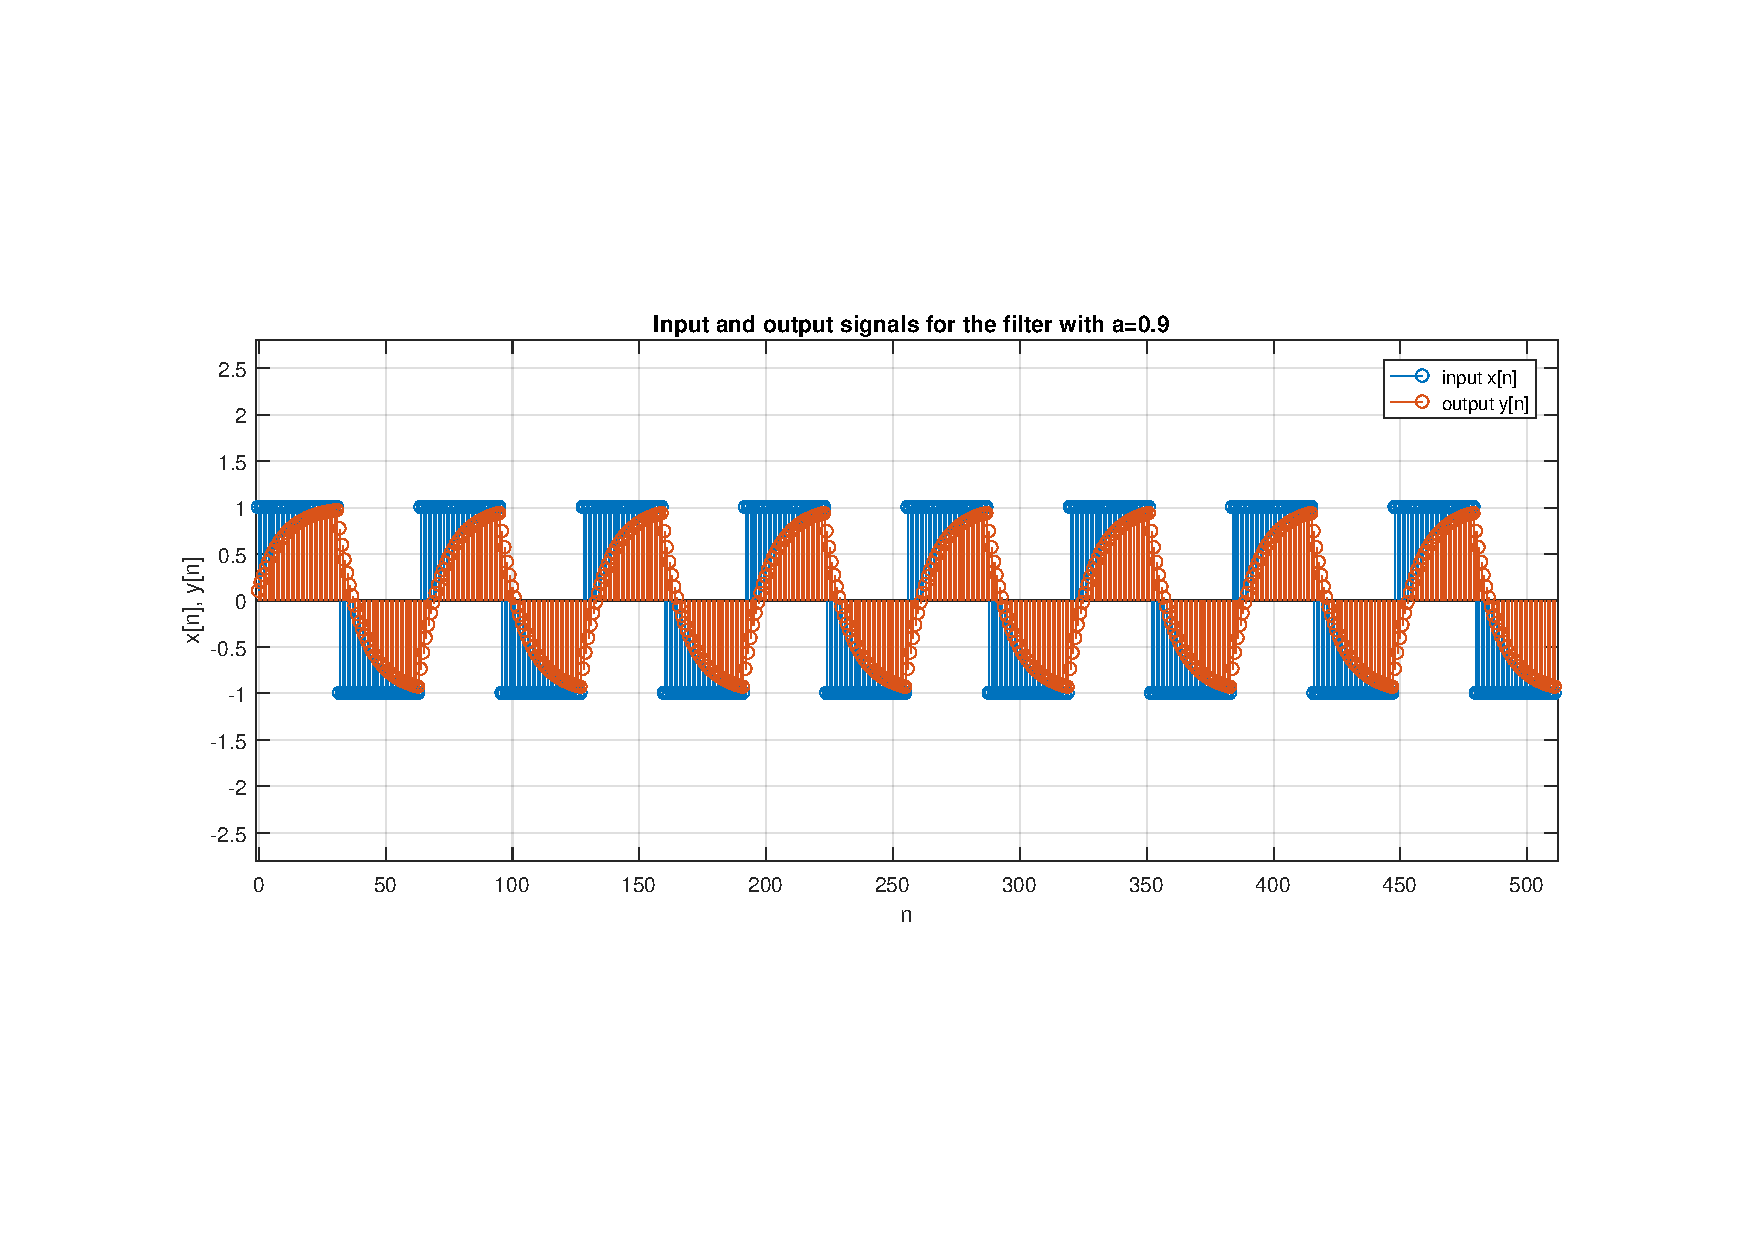
\includegraphics[trim={2.5cm 5cm 2.5cm 5cm}, clip, width=0.75\linewidth]{io_sw_7}
	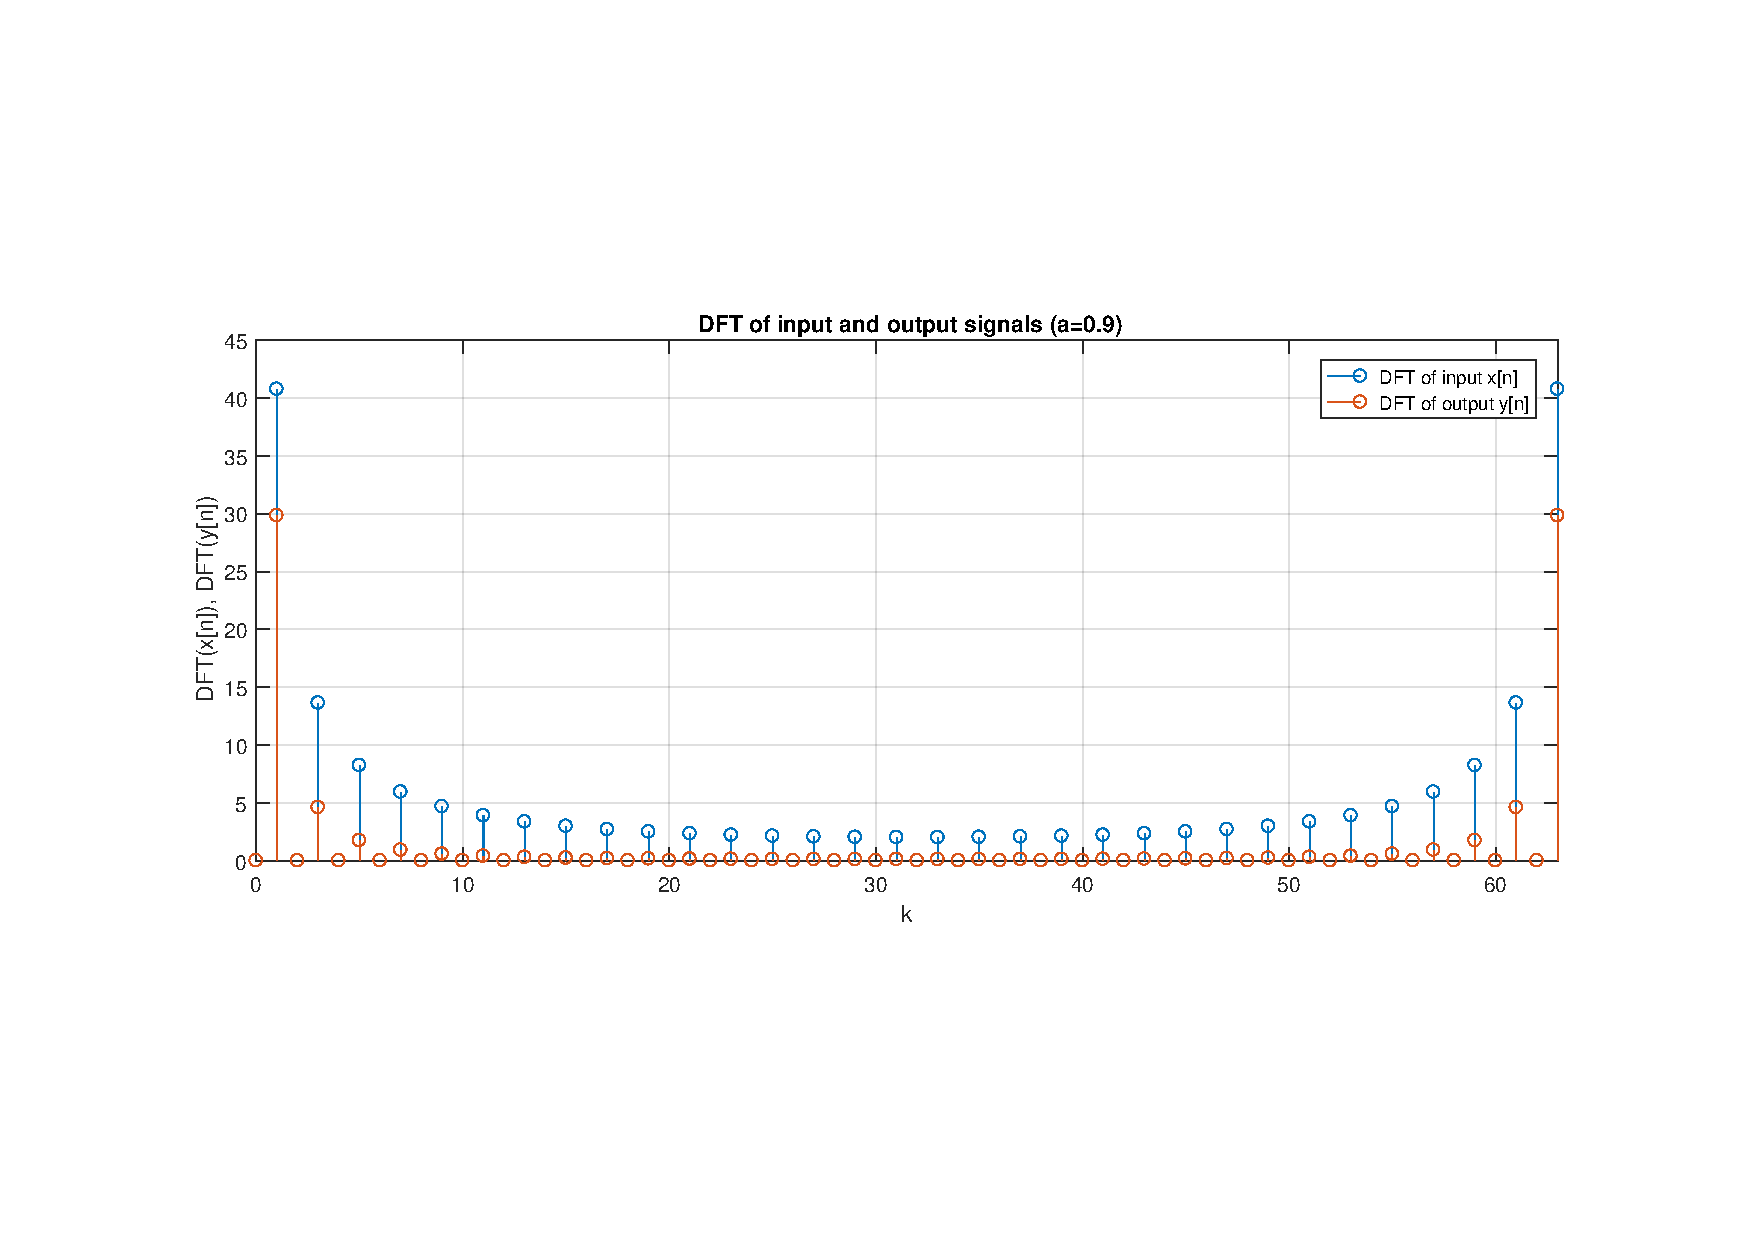
\includegraphics[trim={2.5cm 5cm 2.5cm 5cm}, clip, width=0.75\linewidth]{dft_sw_7}
	\caption{Input and output of the filter and their DFT, square wave input, $a=0.9$}
	\label{fig:t1_io_sw_7}
\end{figure}


\begin{figure} [H]
	\centering
	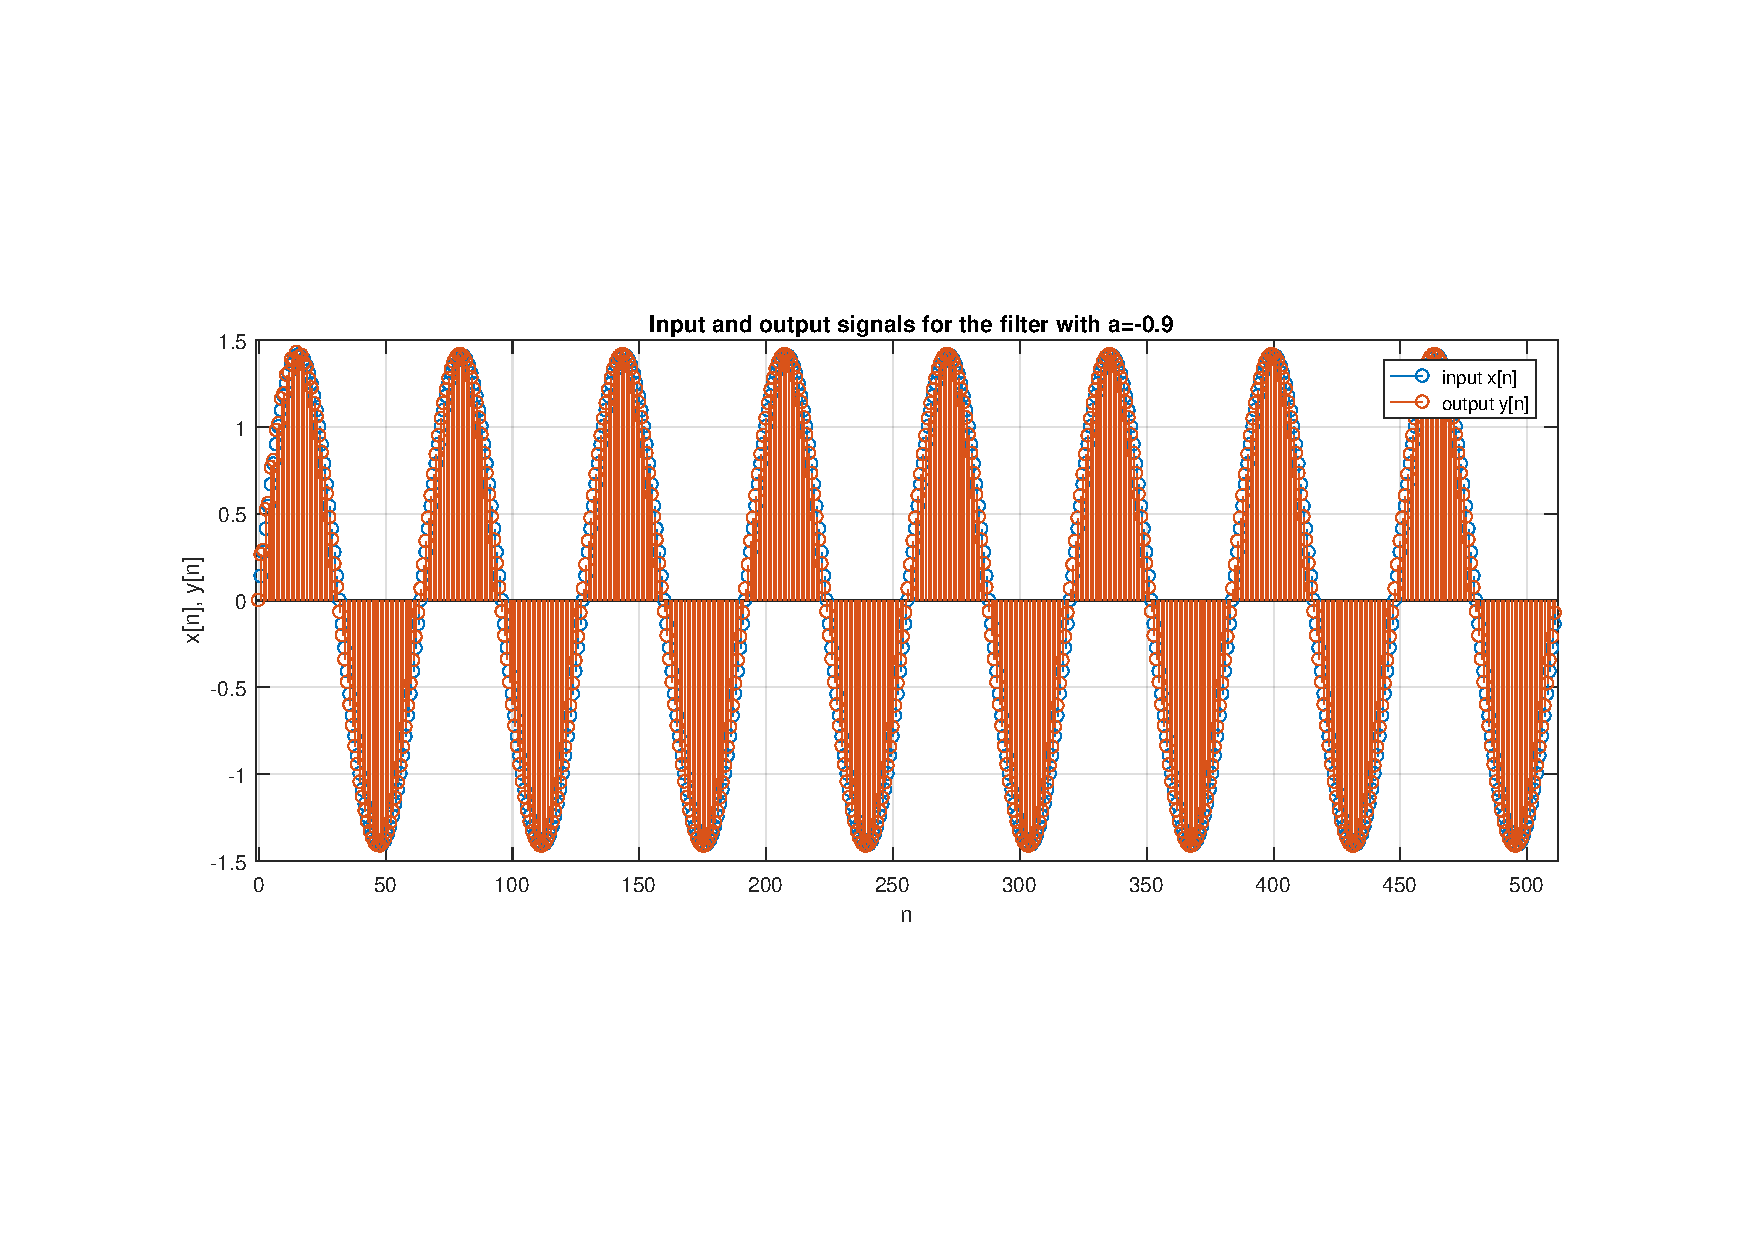
\includegraphics[trim={2.5cm 5cm 2.5cm 5cm}, clip, width=0.75\linewidth]{io_sin_1}
	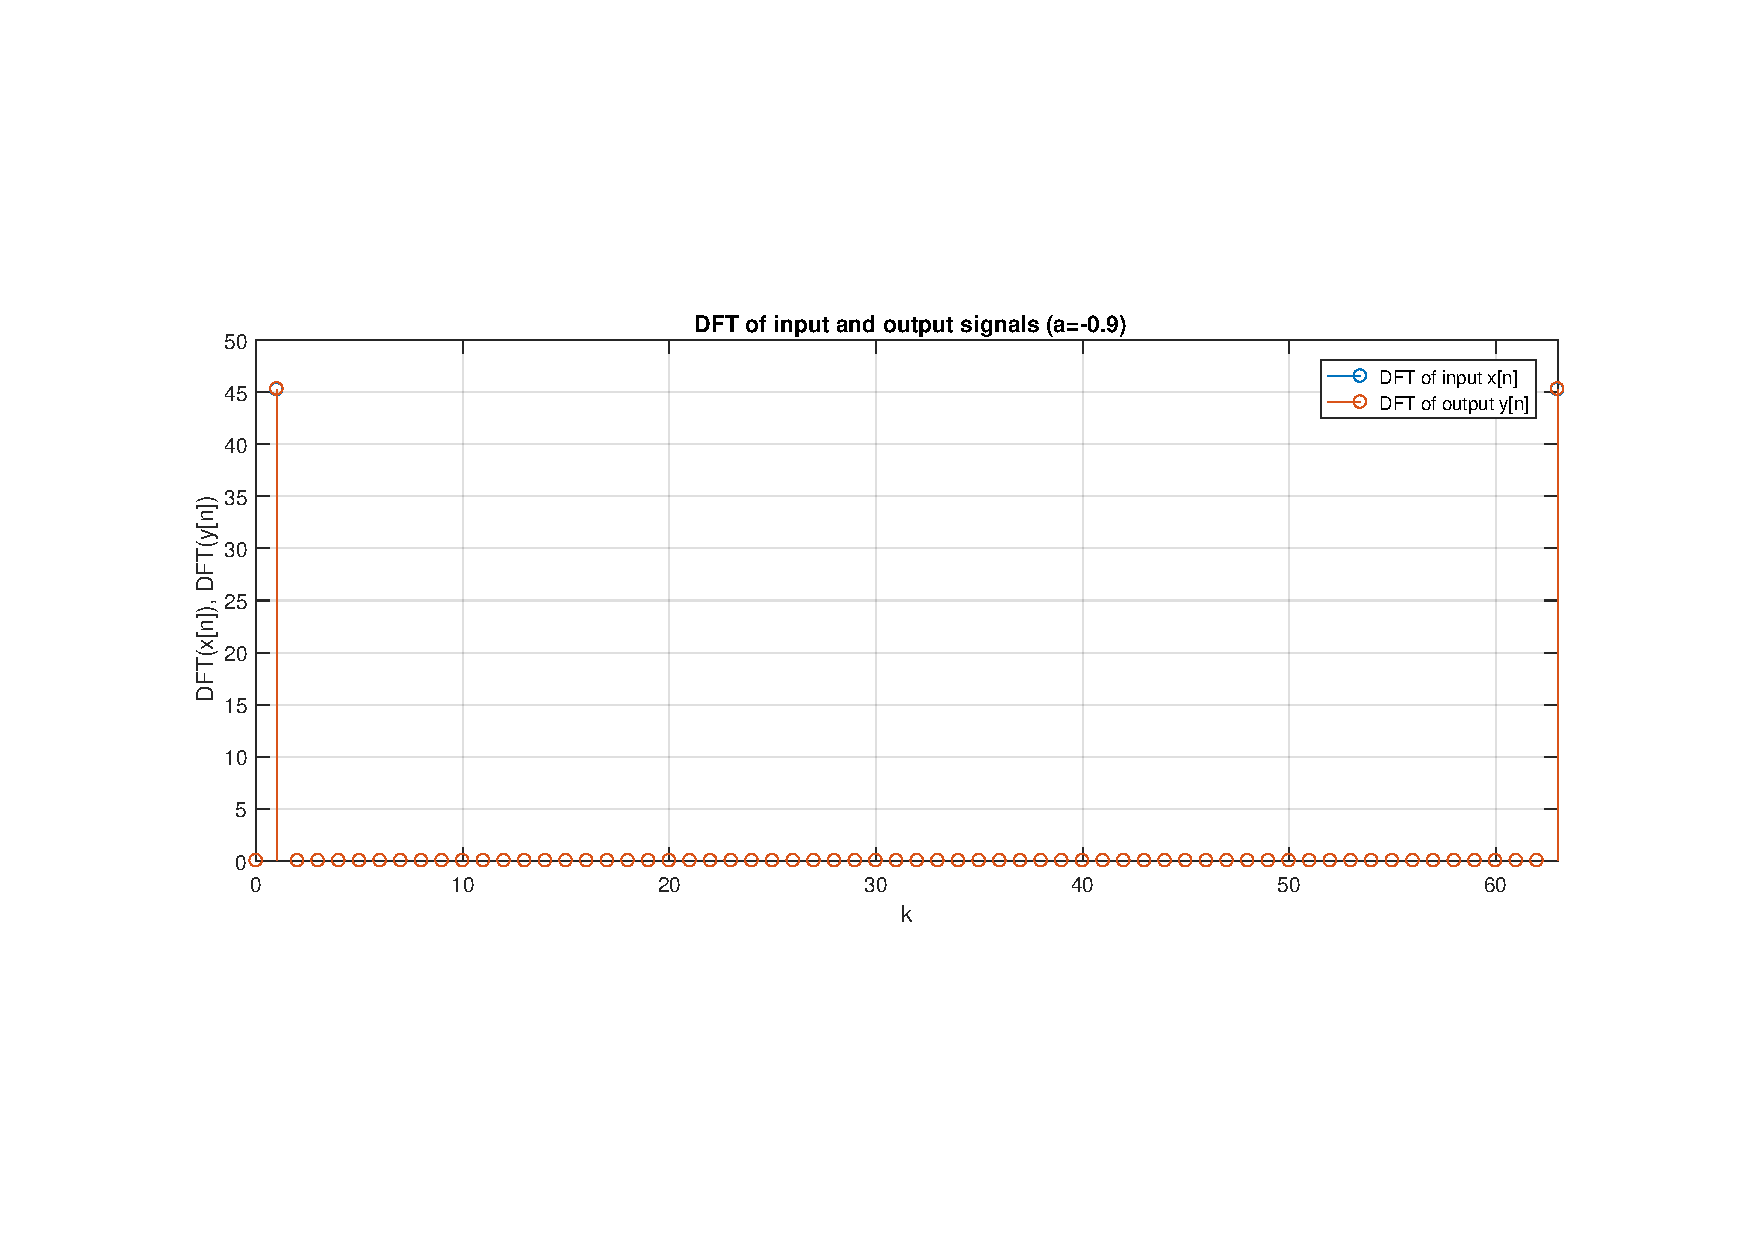
\includegraphics[trim={2.5cm 5cm 2.5cm 5cm}, clip, width=0.75\linewidth]{dft_sin_1}
	\caption{Input and output of the filter and their DFT, sinusoidal wave input, $a=-0.9$ - little differences between input and output}
	\label{fig:t1_io_sin_1}
\end{figure}
\begin{figure} [H]
	\centering
	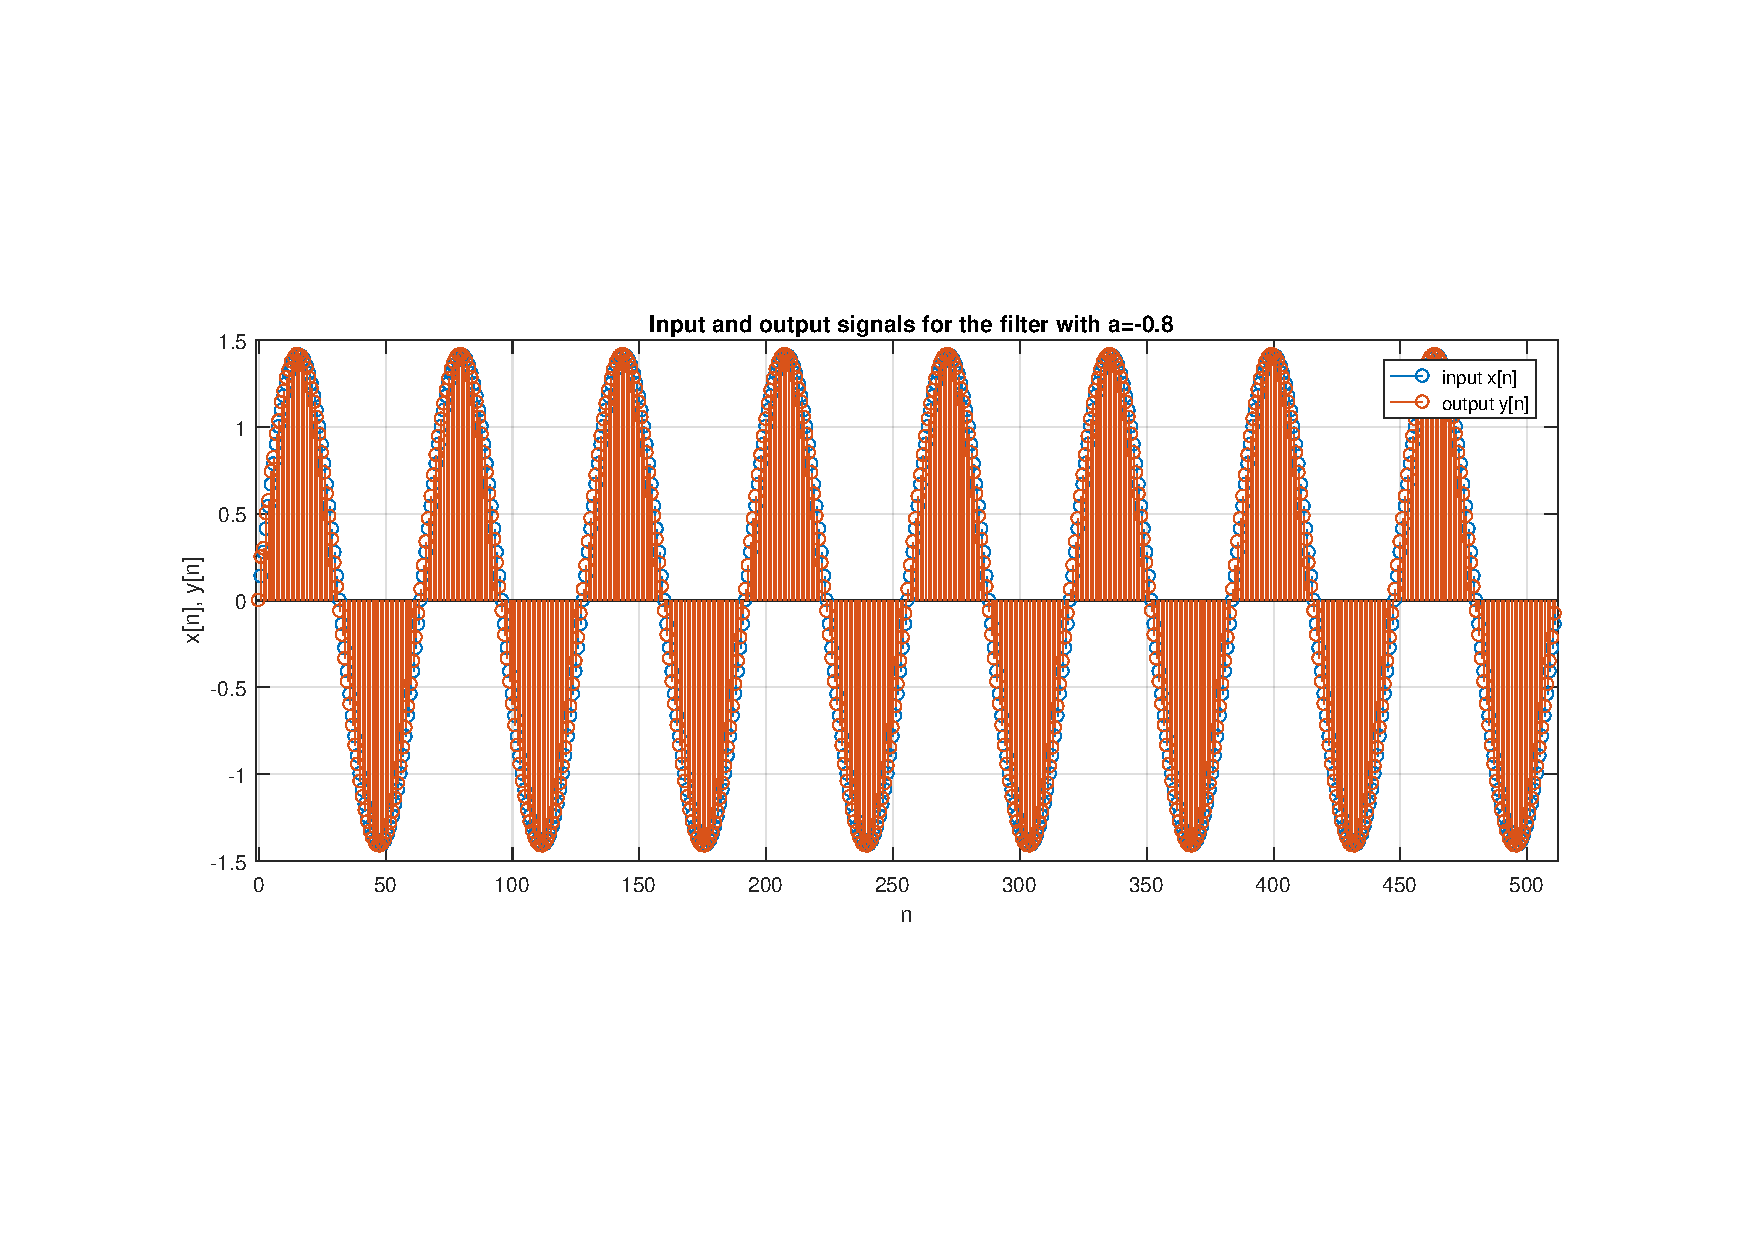
\includegraphics[trim={2.5cm 5cm 2.5cm 5cm}, clip, width=0.75\linewidth]{io_sin_2}
	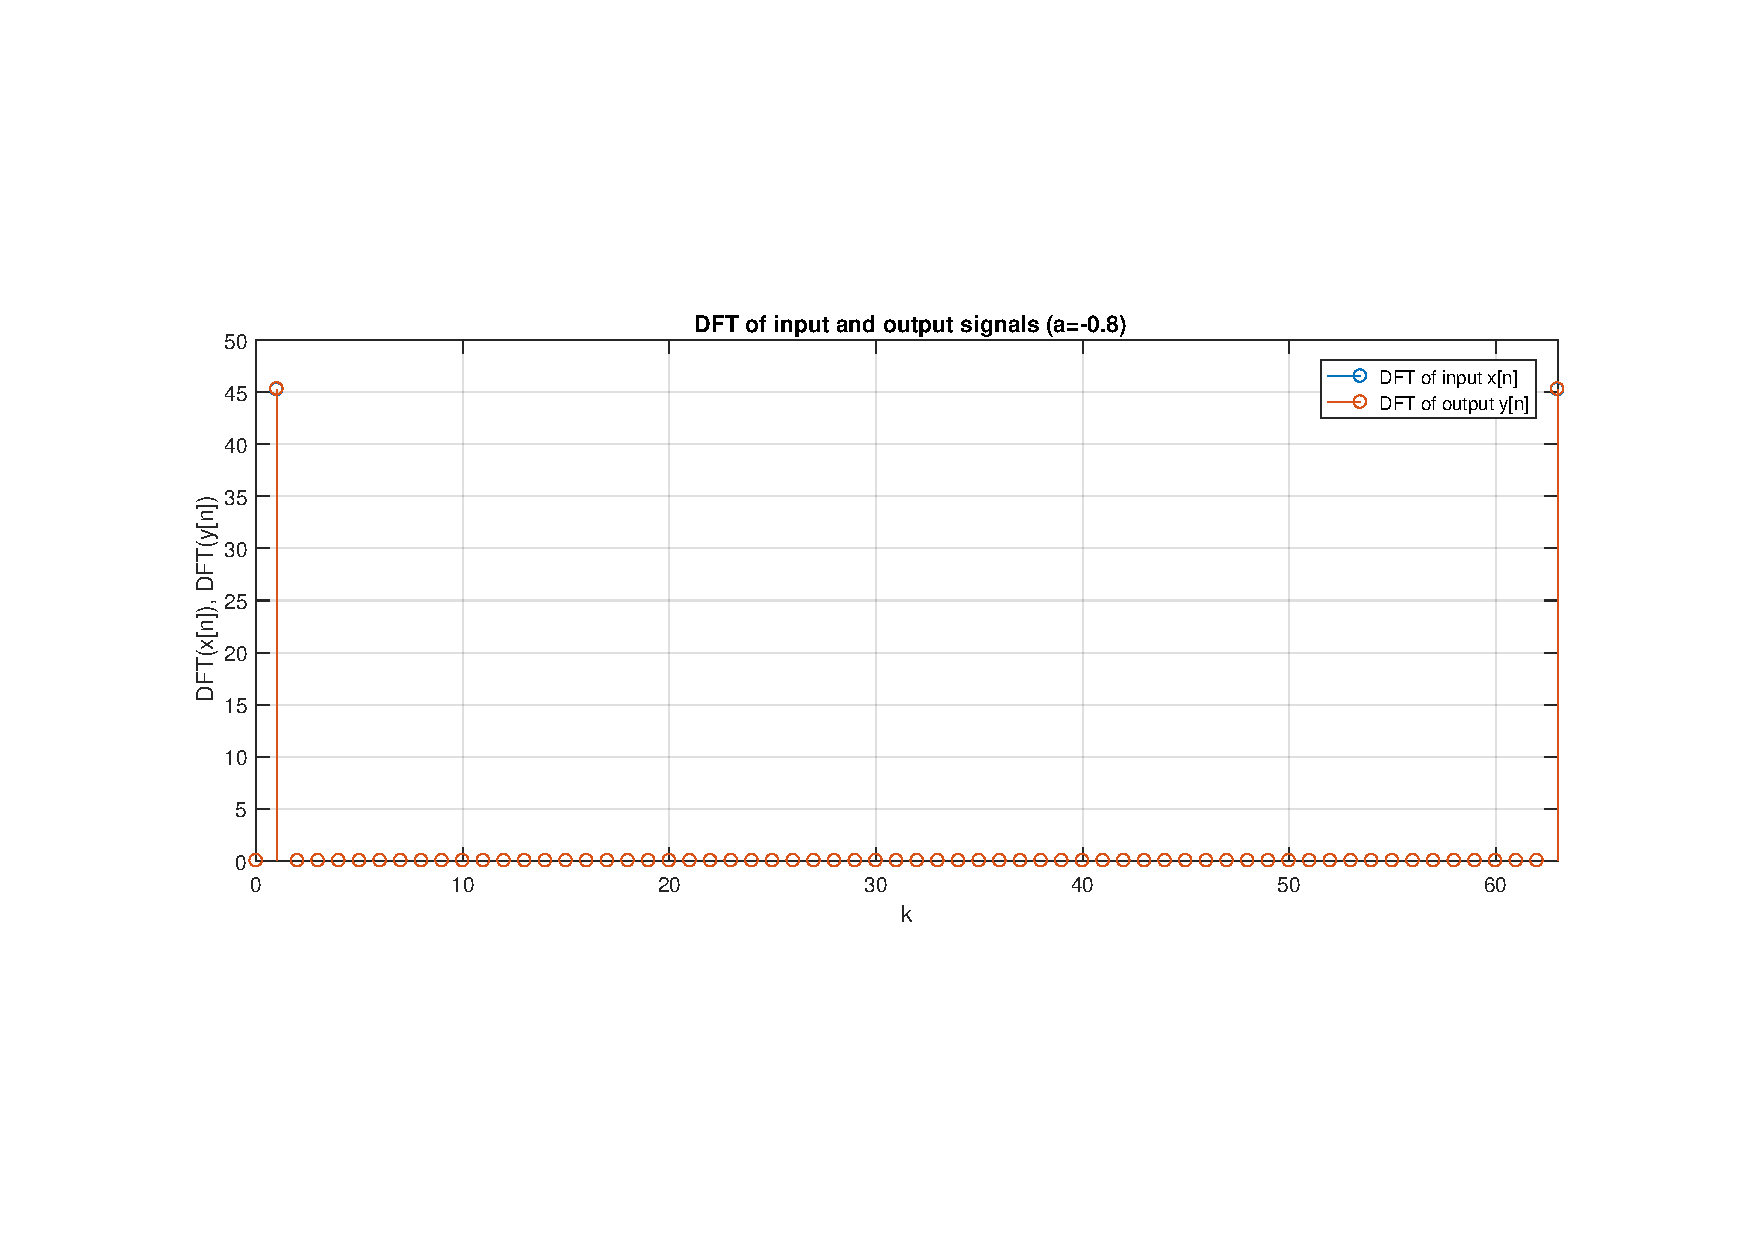
\includegraphics[trim={2.5cm 5cm 2.5cm 5cm}, clip, width=0.75\linewidth]{dft_sin_2}
	\caption{Input and output of the filter and their DFT, sinusoidal wave input, $a=-0.8$}
	\label{fig:t1_io_sin_2}
\end{figure}
\begin{figure} [H]
	\centering
	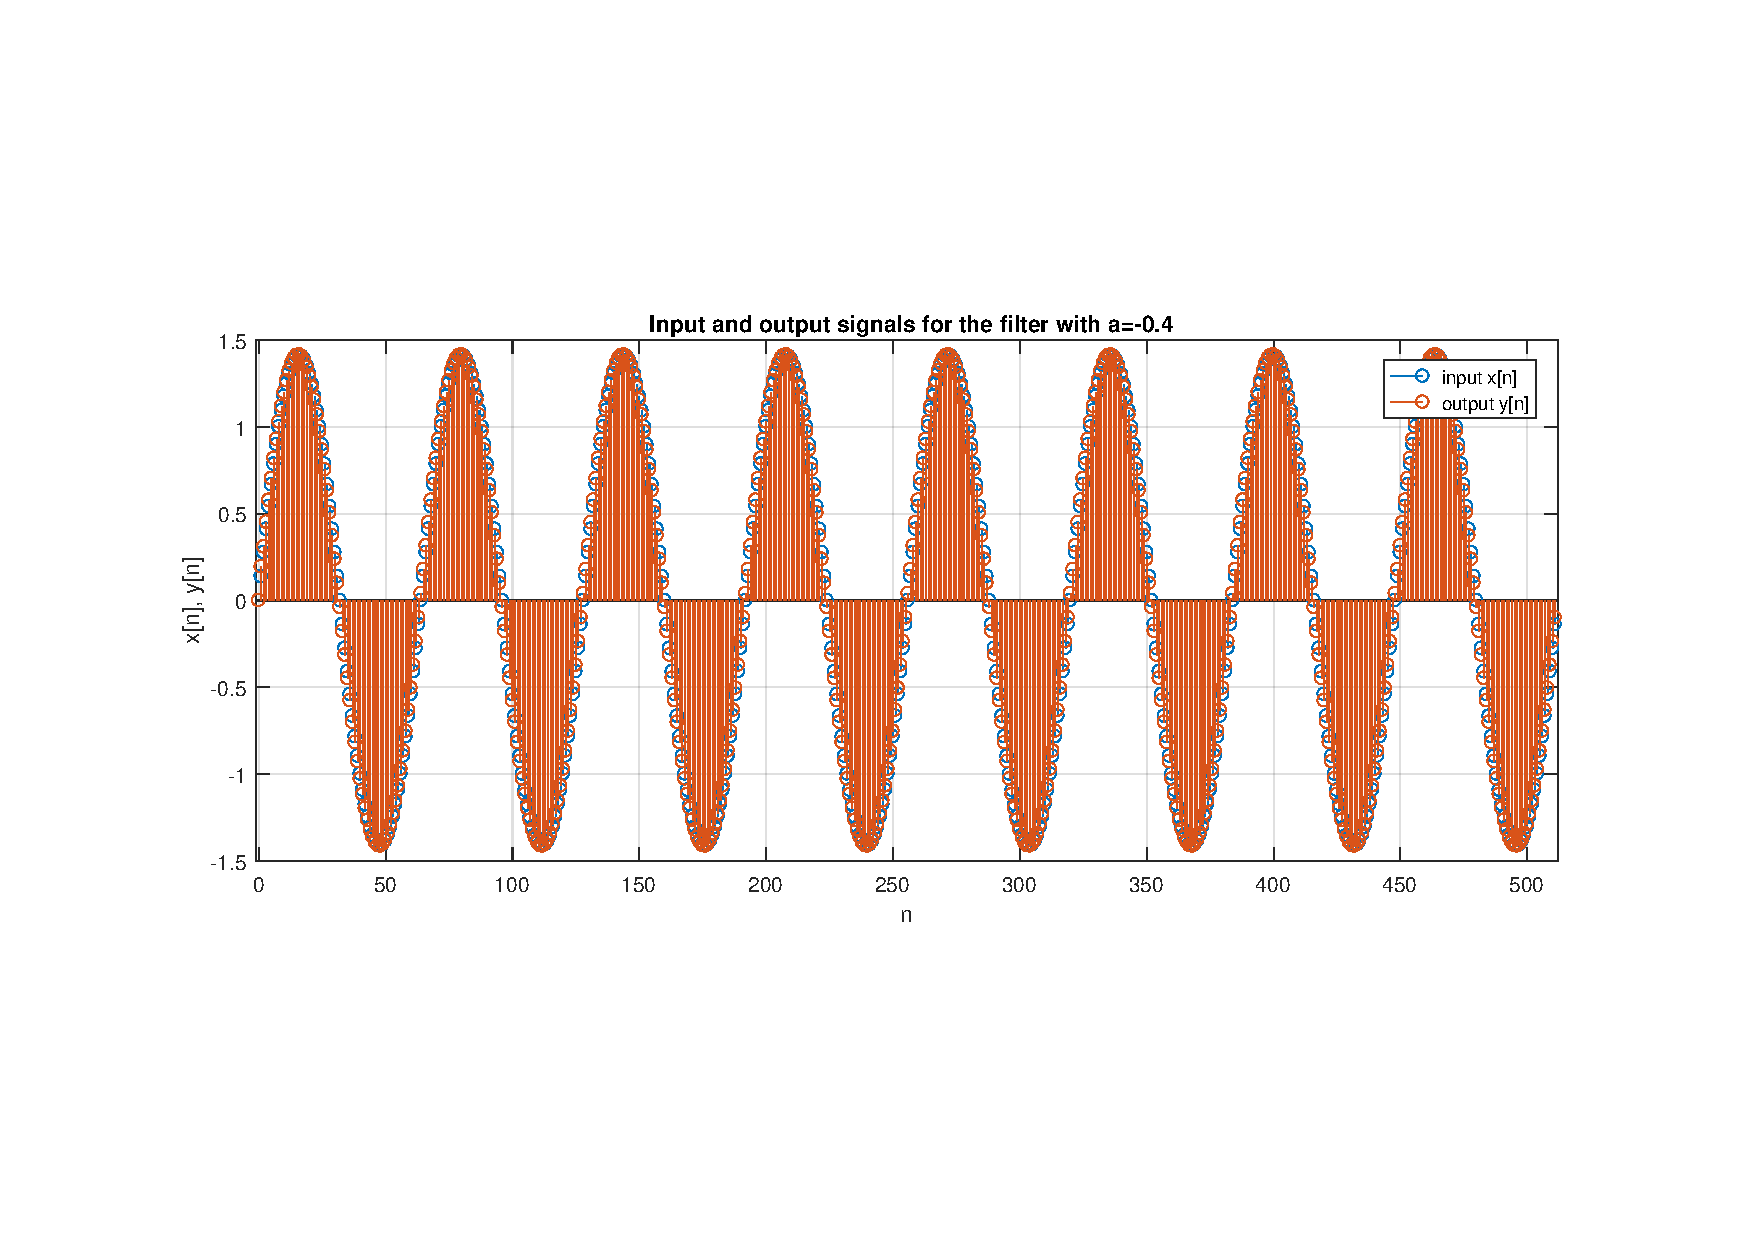
\includegraphics[trim={2.5cm 5cm 2.5cm 5cm}, clip, width=0.75\linewidth]{io_sin_3}
	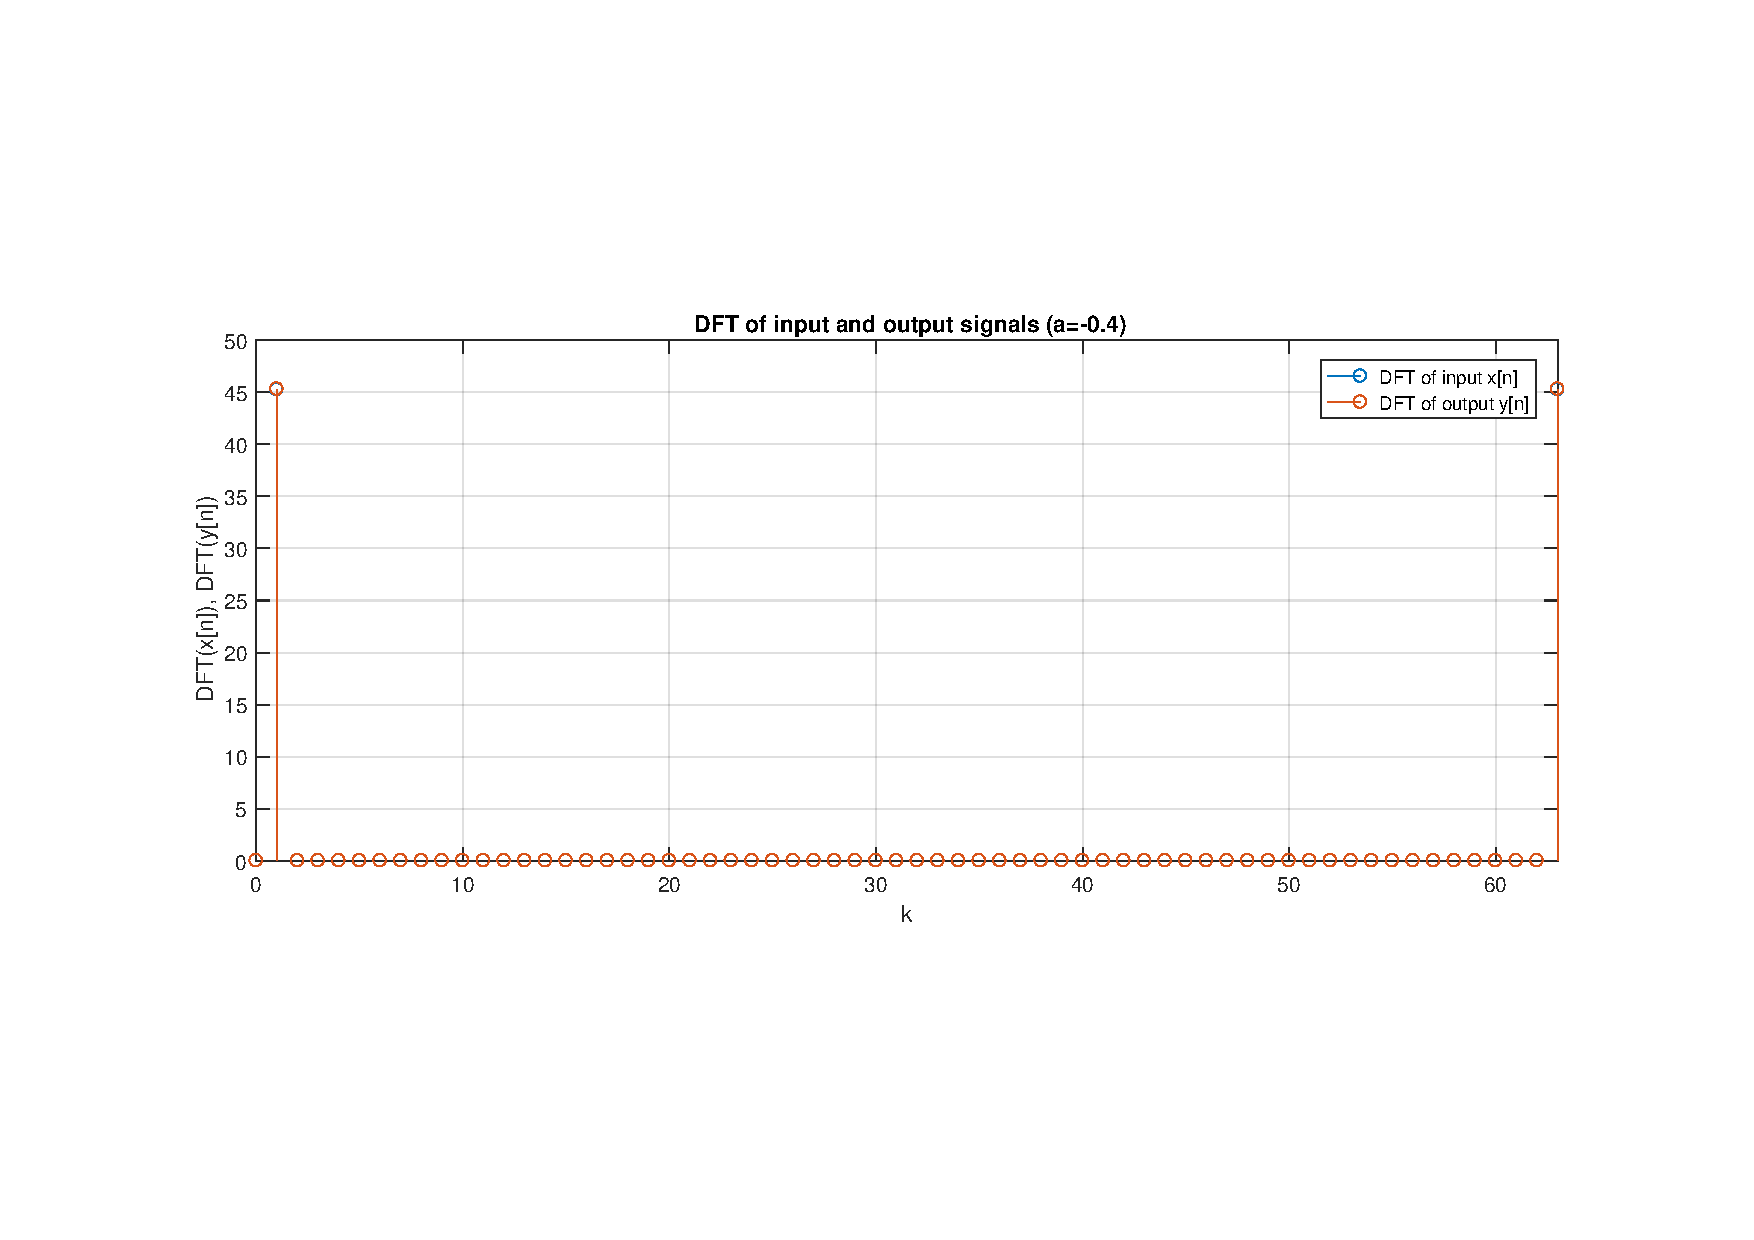
\includegraphics[trim={2.5cm 5cm 2.5cm 5cm}, clip, width=0.75\linewidth]{dft_sin_3}
		\caption{Input and output of the filter and their DFT, sinusoidal wave input, $a=-0.4$}
	\label{fig:t1_io_sin_3}
\end{figure}
\begin{figure} [H]
	\centering
	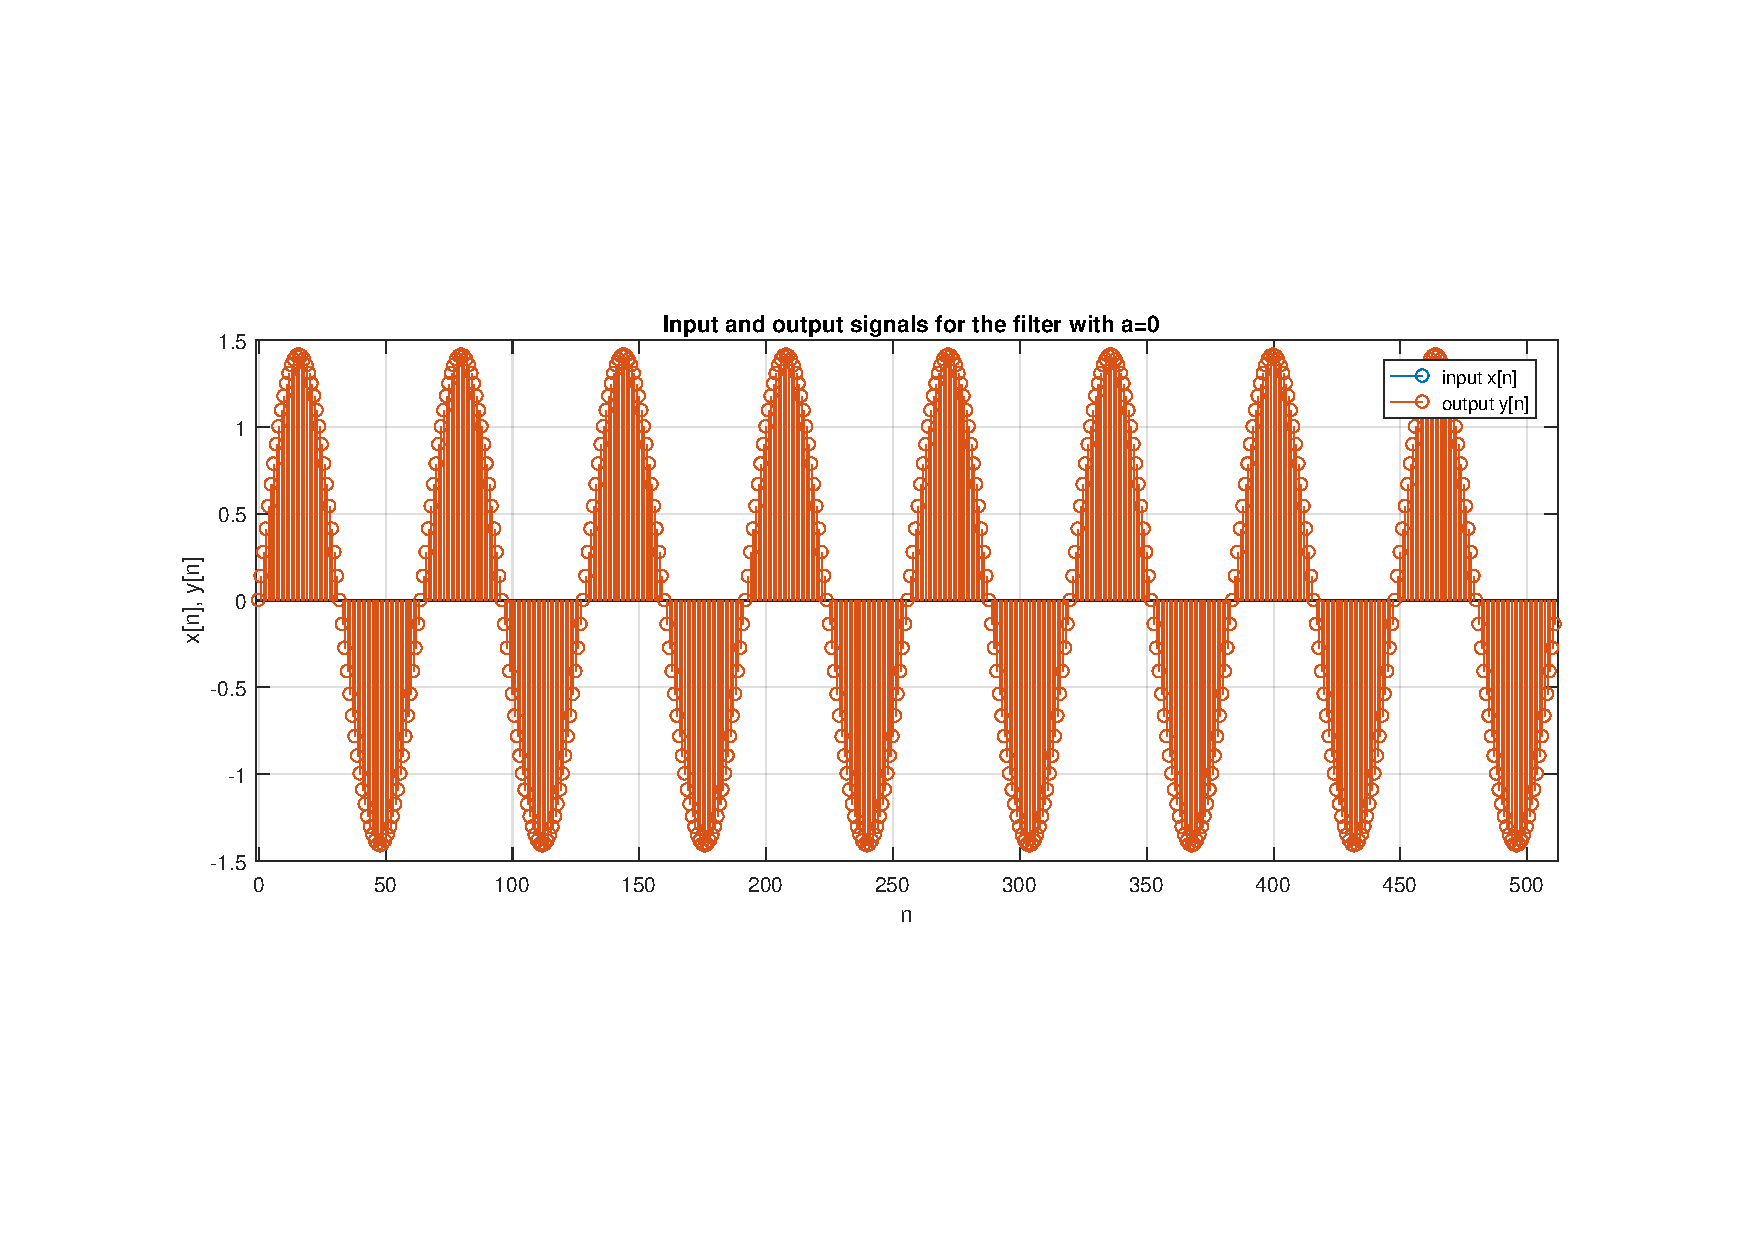
\includegraphics[trim={2.5cm 5cm 2.5cm 5cm}, clip, width=0.75\linewidth]{io_sin_4}
	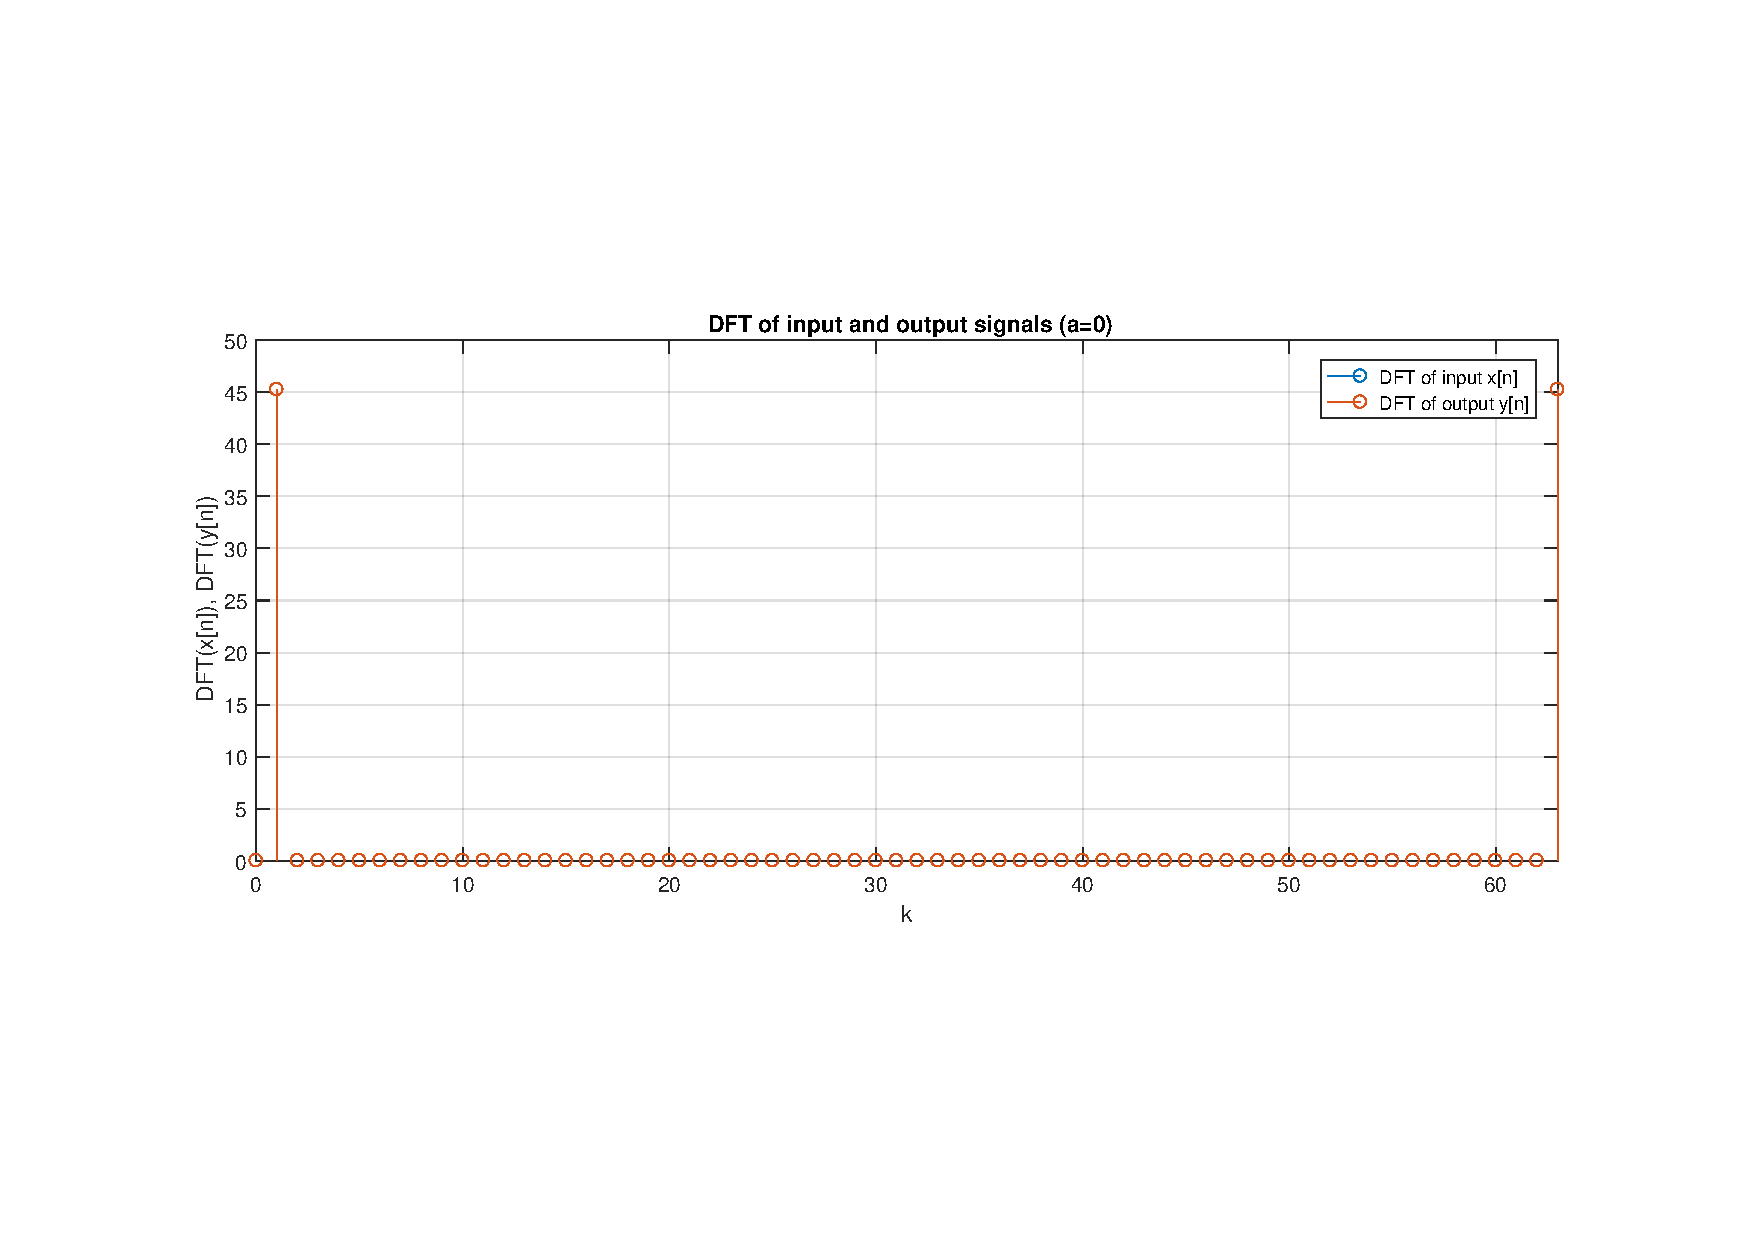
\includegraphics[trim={2.5cm 5cm 2.5cm 5cm}, clip, width=0.75\linewidth]{dft_sin_4}
	\caption{Input and output of the filter and their DFT, sinusoidal wave input, $a=0$ - the output is equal to the input, unitary tf}
	\label{fig:t1_io_sin_4}
\end{figure}
\begin{figure} [H]
	\centering
	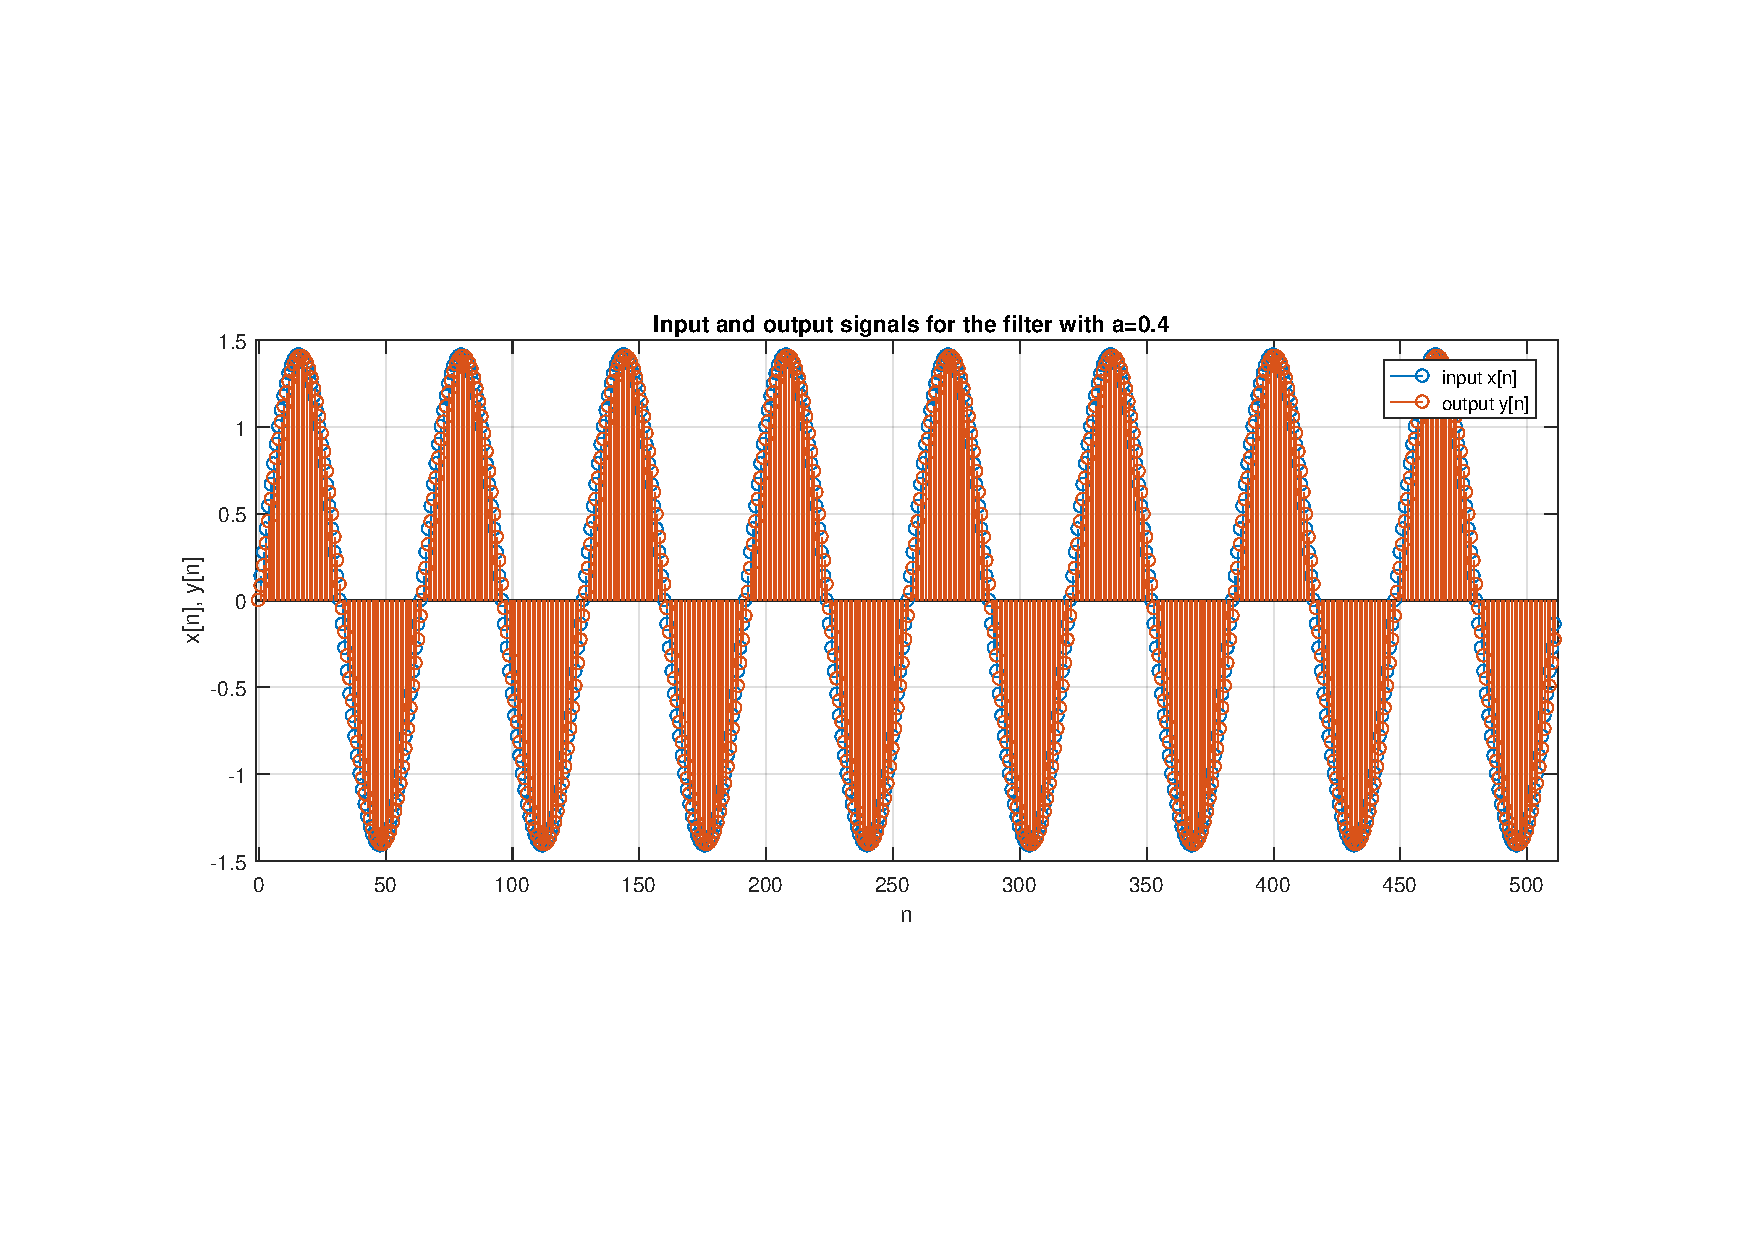
\includegraphics[trim={2.5cm 5cm 2.5cm 5cm}, clip, width=0.75\linewidth]{io_sin_5}
	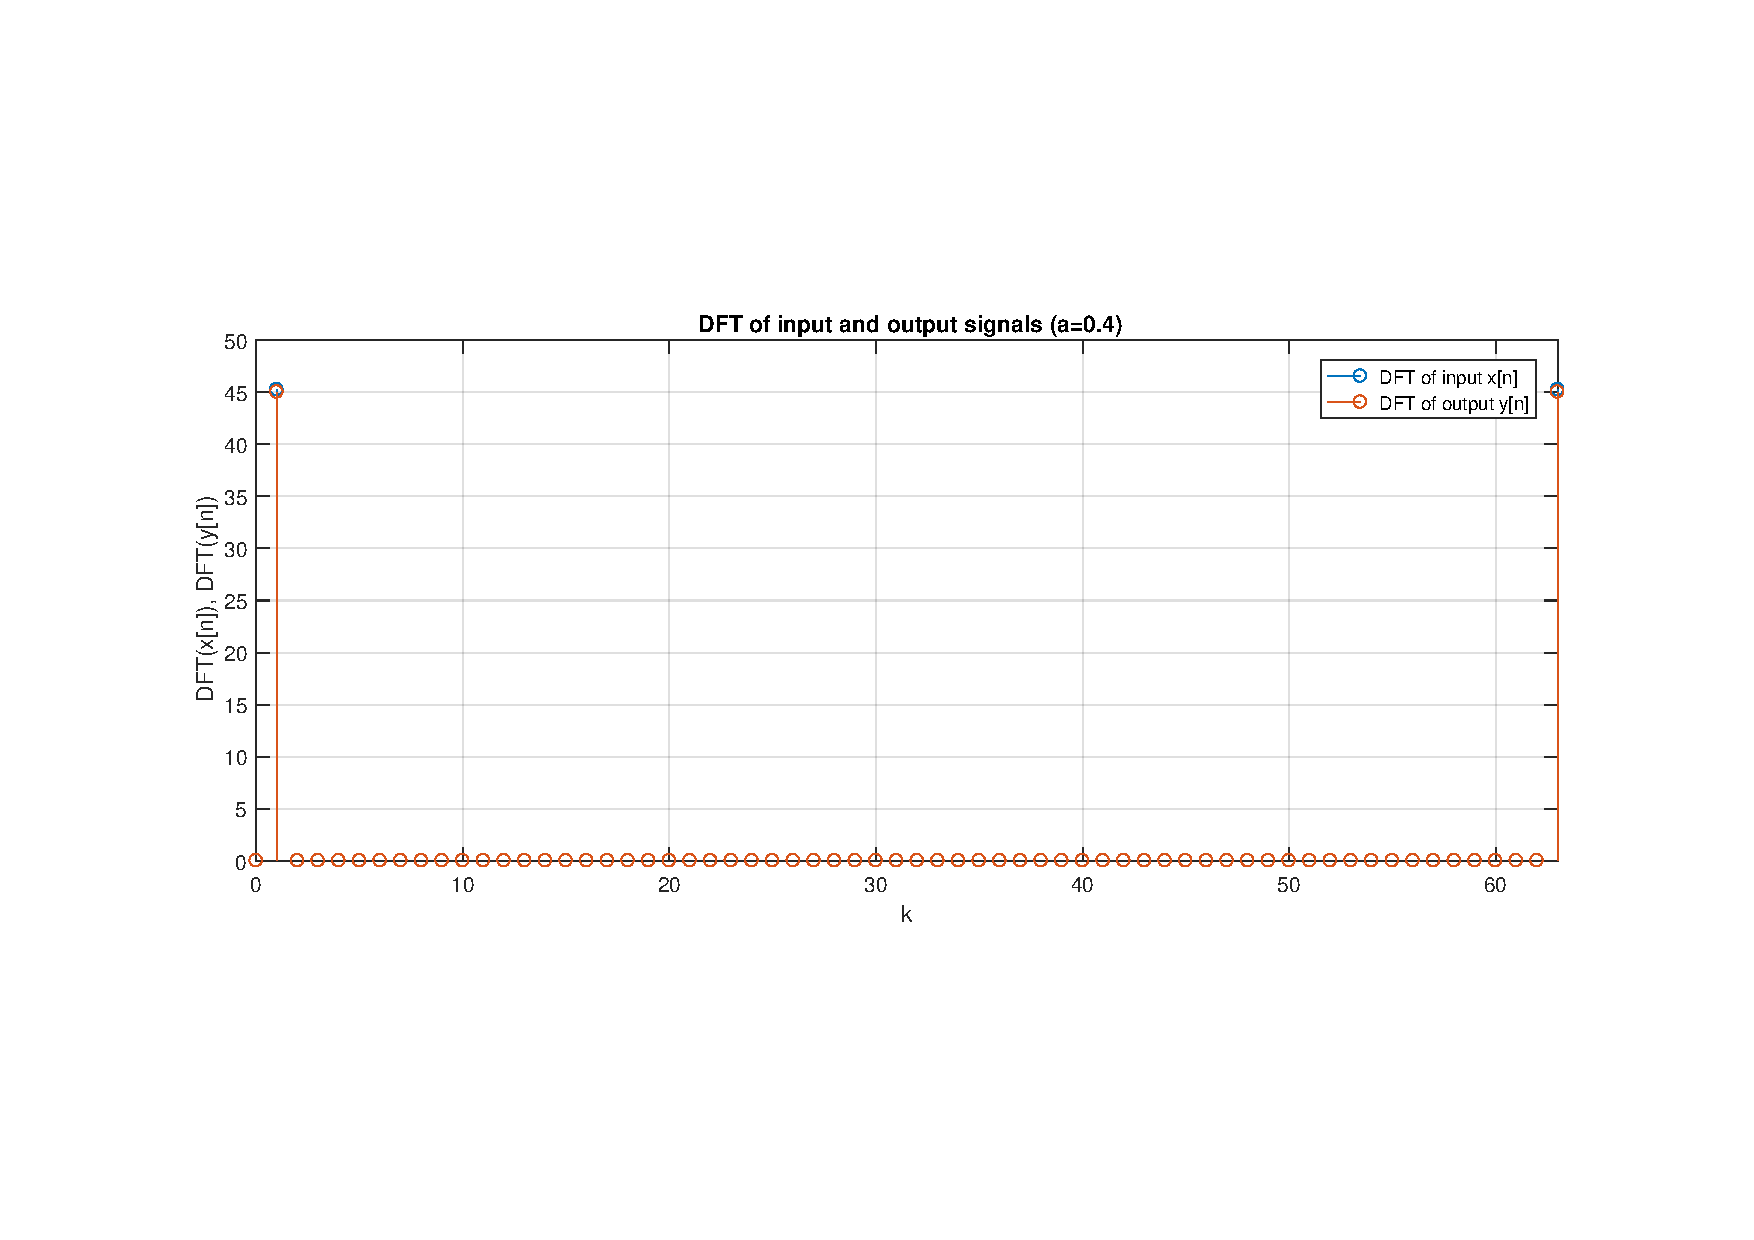
\includegraphics[trim={2.5cm 5cm 2.5cm 5cm}, clip, width=0.75\linewidth]{dft_sin_5}
		\caption{Input and output of the filter and their DFT, sinusoidal wave input, $a=0.4$}
	\label{fig:t1_io_sin_5}
\end{figure}
\begin{figure} [H]
	\centering
	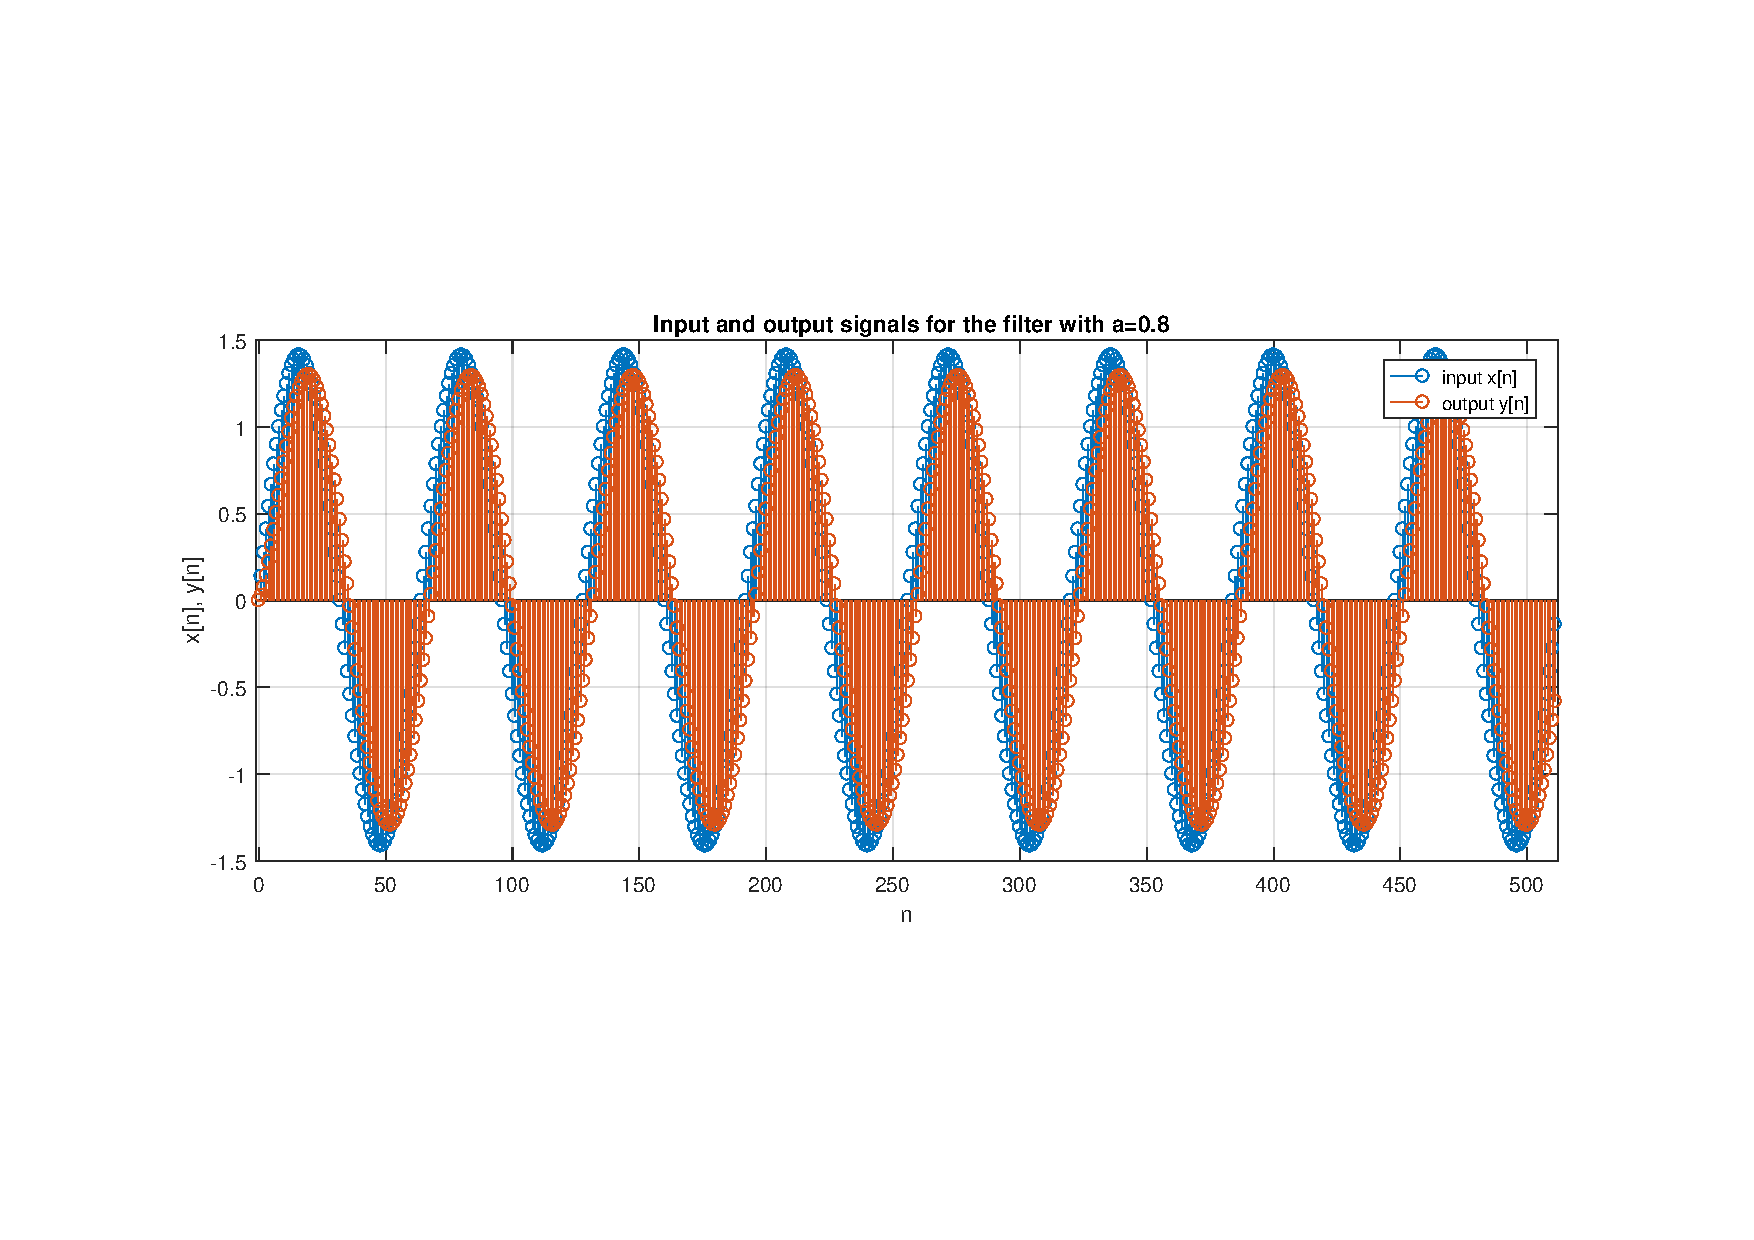
\includegraphics[trim={2.5cm 5cm 2.5cm 5cm}, clip, width=0.75\linewidth]{io_sin_6}
	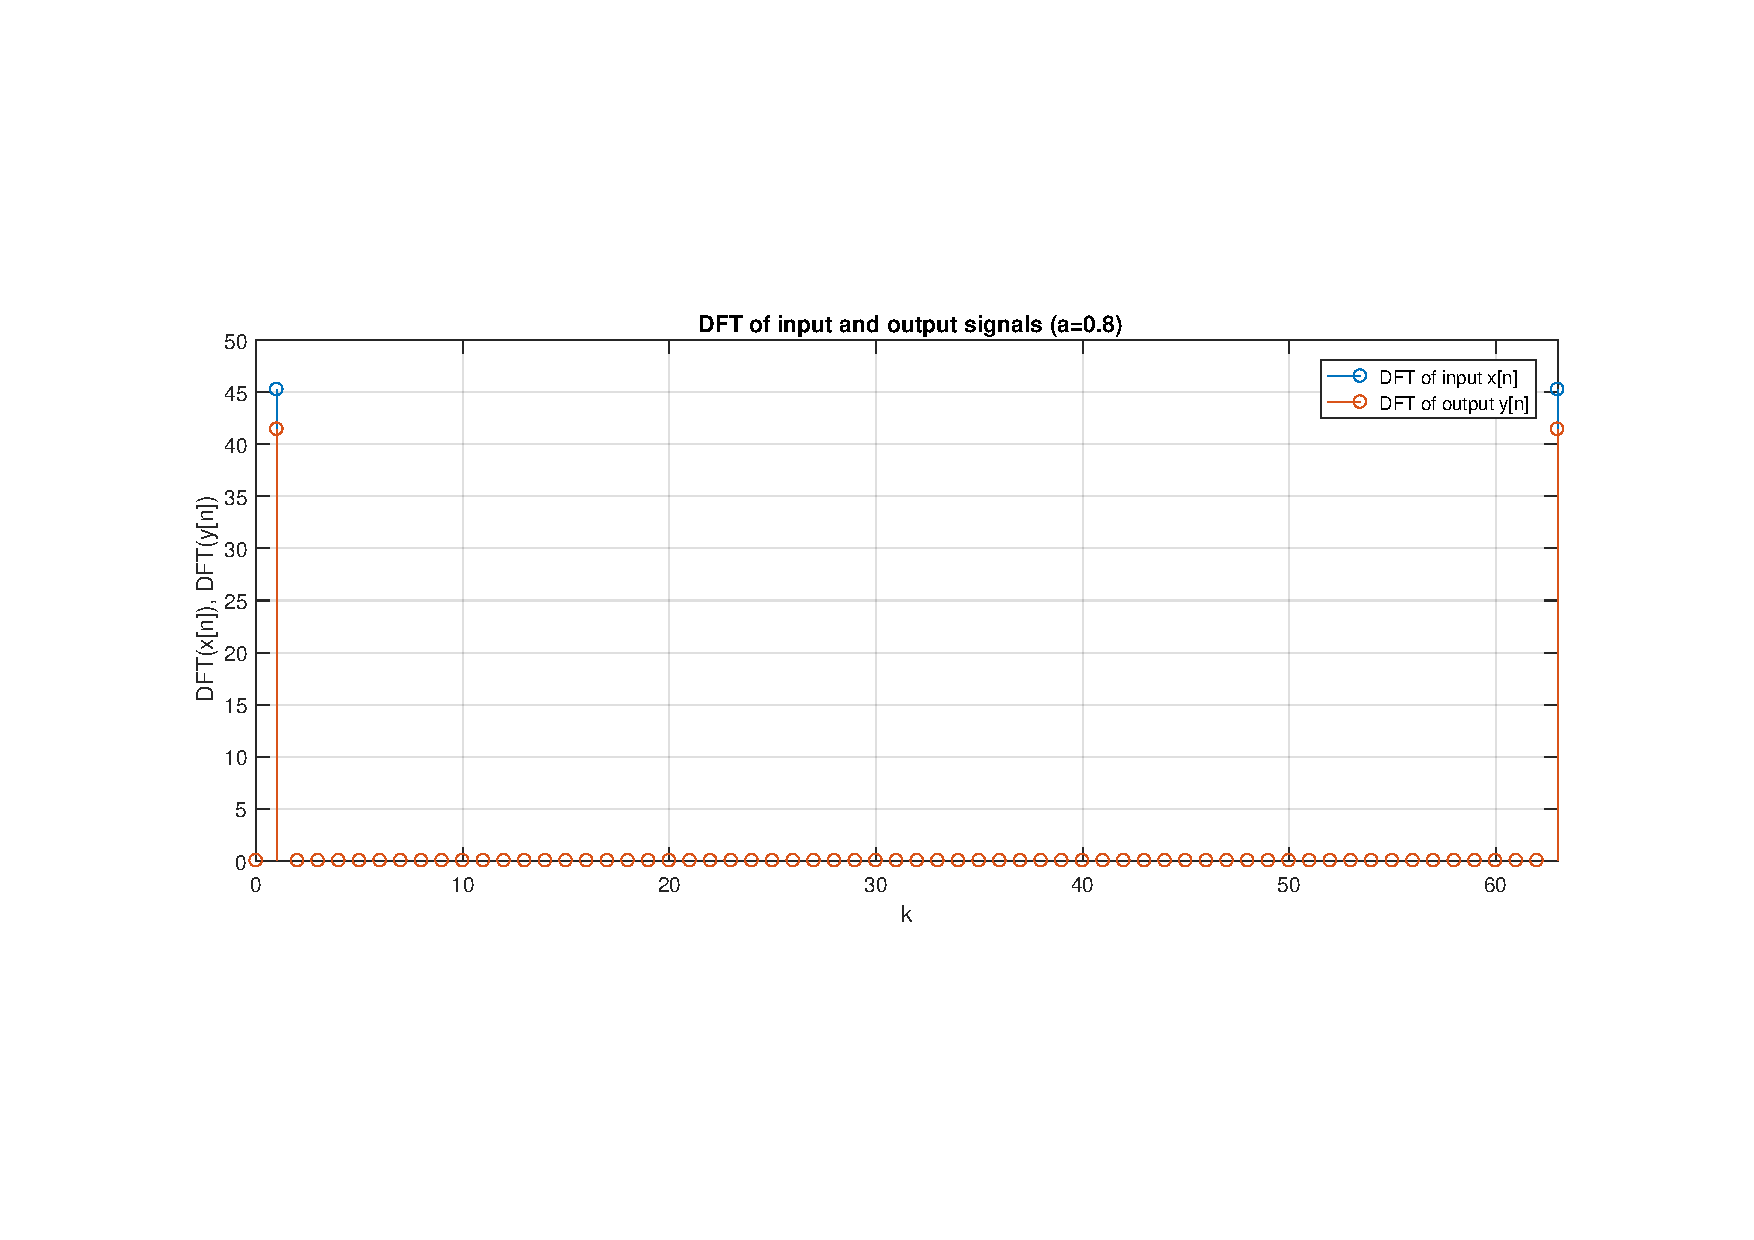
\includegraphics[trim={2.5cm 5cm 2.5cm 5cm}, clip, width=0.75\linewidth]{dft_sin_6}
	\caption{Input and output of the filter and their DFT, sinusoidal wave input, $a=0.8$}
	\label{fig:t1_io_sin_6}
\end{figure}
\begin{figure} [H]
	\centering
	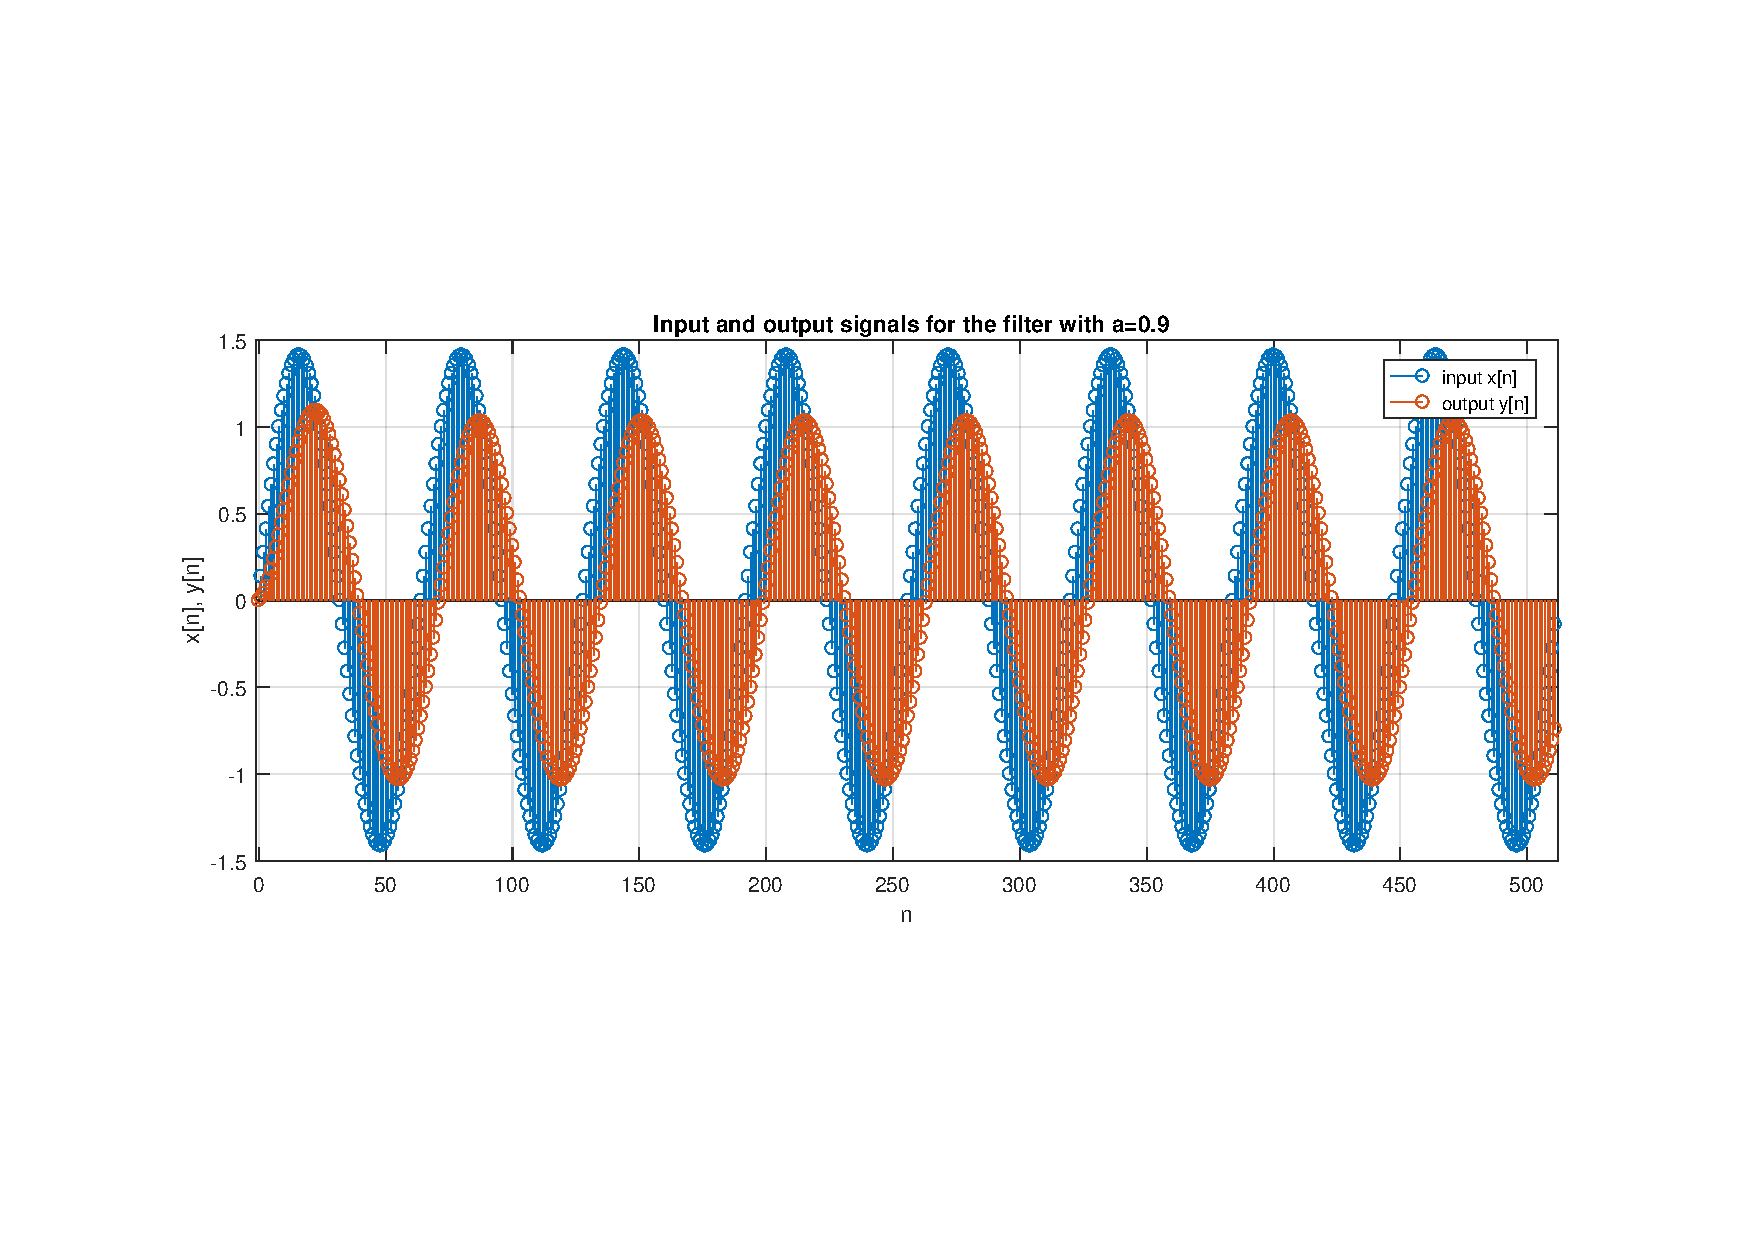
\includegraphics[trim={2.5cm 5cm 2.5cm 5cm}, clip, width=0.75\linewidth]{io_sin_7}
	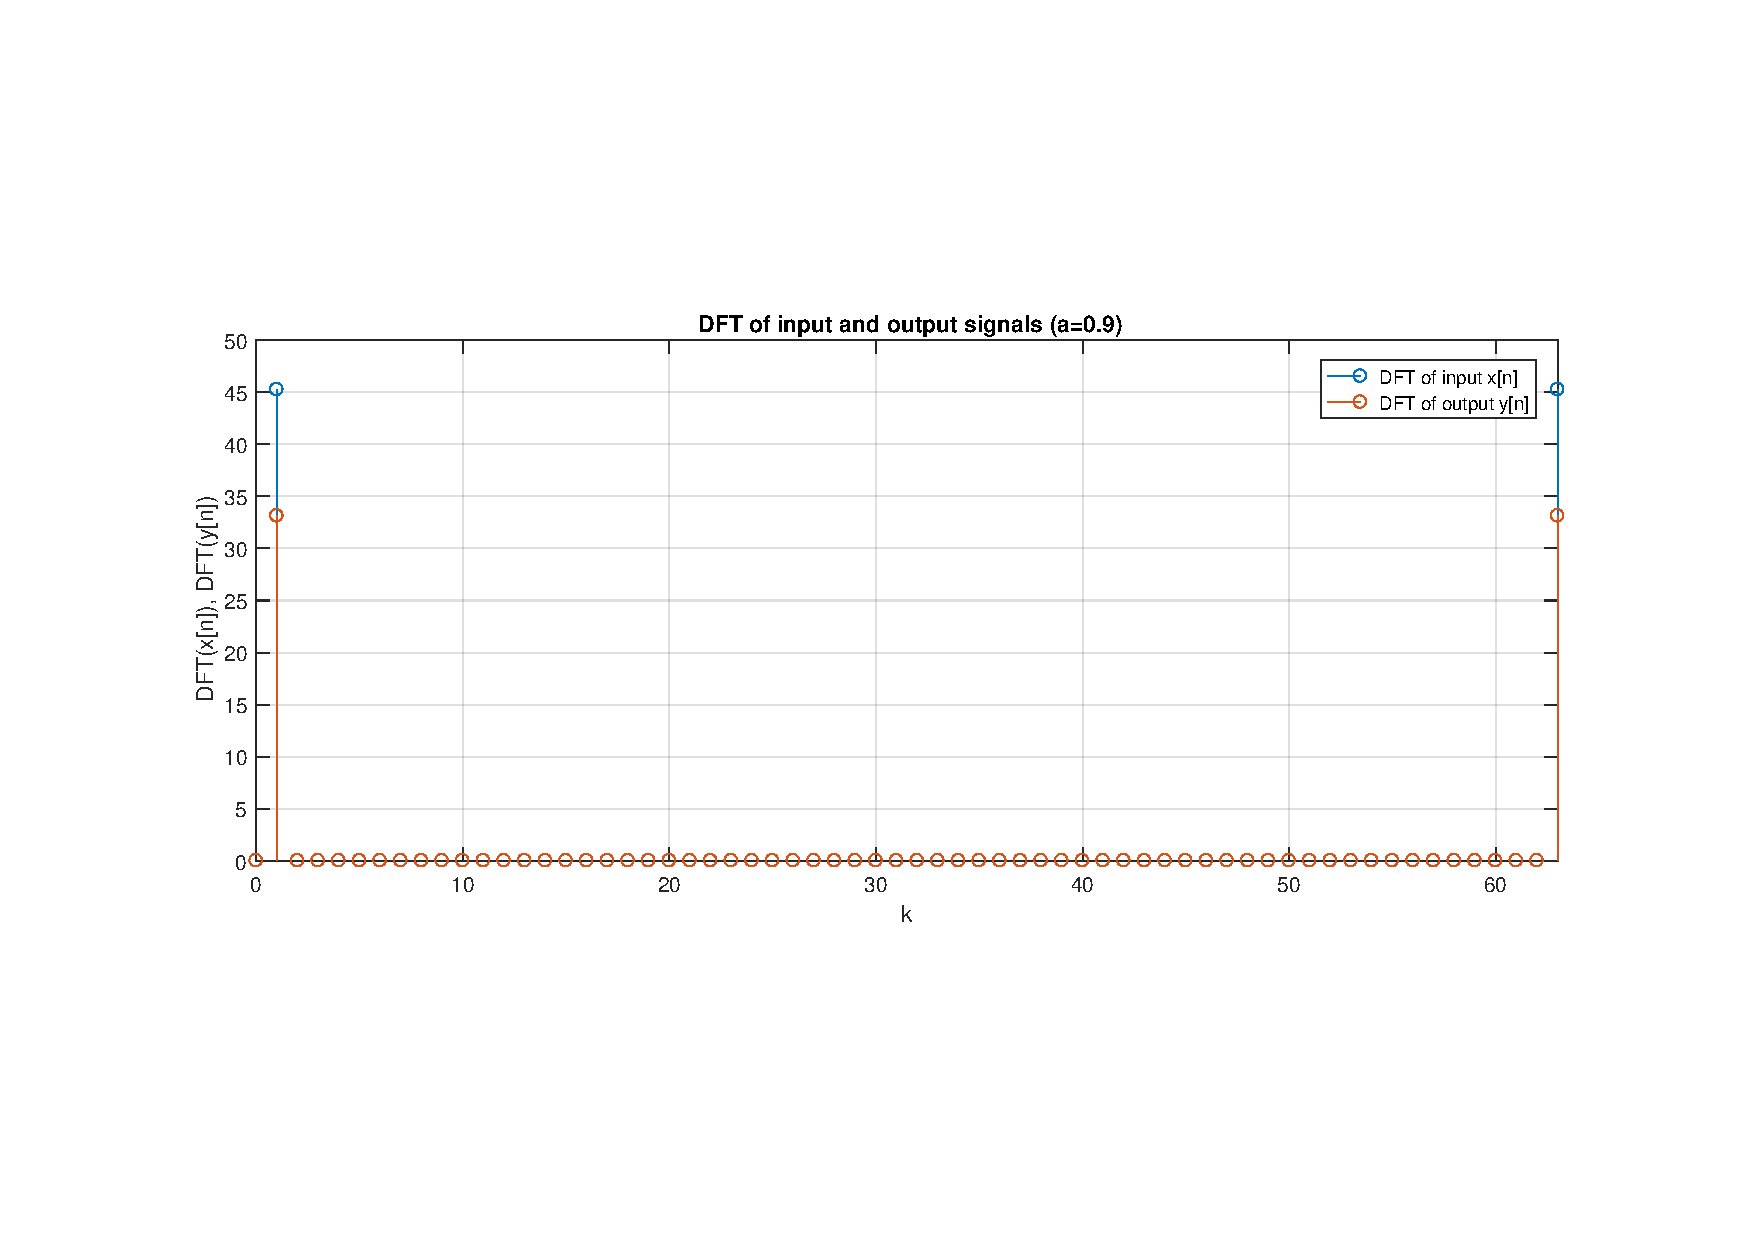
\includegraphics[trim={2.5cm 5cm 2.5cm 5cm}, clip, width=0.75\linewidth]{dft_sin_7}
	\caption{Input and output of the filter and their DFT, sinusoidal wave input, $a=0.9$ - the sinusoid on the output is phase shifted and attenuated}
	\label{fig:t1_io_sin_7}
\end{figure}
